% Options for packages loaded elsewhere
\PassOptionsToPackage{unicode}{hyperref}
\PassOptionsToPackage{hyphens}{url}
\documentclass[a4paper]{extarticle}
\usepackage{fix-cm}
\usepackage[fontsize=13pt]{scrextend}
\usepackage{xcolor}
\usepackage[margin=2.5cm,top=2.5cm,bottom=2.5cm,left=2.5cm,right=2.5cm,headheight=1.25cm,headsep=0.5cm,footskip=1.25cm]{geometry}
\usepackage{amsmath,amssymb}
\setcounter{secnumdepth}{-\maxdimen} % remove section numbering
\usepackage{iftex}
\ifPDFTeX
  \usepackage[T5,T1]{fontenc}
  \usepackage[utf8]{inputenc}
  \usepackage{textcomp} % provide euro and other symbols
  \IfFileExists{newtxtext.sty}{\usepackage{newtxtext,newtxmath}}{\usepackage{lmodern}}
\else % if luatex or xetex
  \usepackage{fontspec}
  \IfFontExistsTF{Times New Roman}{\setmainfont{Times New Roman}}{\setmainfont{TeX Gyre Termes}}
  \setmonofont{Consolas}[Scale=MatchLowercase]
\fi
% Use upquote if available, for straight quotes in verbatim environments
\IfFileExists{upquote.sty}{\usepackage{upquote}}{}
\IfFileExists{microtype.sty}{% use microtype if available
  \usepackage[]{microtype}
  \UseMicrotypeSet[protrusion]{basicmath} % disable protrusion for tt fonts
}{}
\makeatletter
\@ifundefined{KOMAClassName}{% if non-KOMA class
  \IfFileExists{parskip.sty}{%
    \usepackage{parskip}
  }{% else
    \setlength{\parindent}{0pt}
    \setlength{\parskip}{6pt plus 2pt minus 1pt}}
}{% if KOMA class
  \KOMAoptions{parskip=half}}
\makeatother
\usepackage{color}
\usepackage{fancyvrb}
\newcommand{\VerbBar}{|}
\newcommand{\VERB}{\Verb[commandchars=\\\{\}]}
\DefineVerbatimEnvironment{Highlighting}{Verbatim}{commandchars=\\\{\},formatcom=\rmfamily}
\RecustomVerbatimEnvironment{verbatim}{Verbatim}{fontsize=\small}
% Add ',fontsize=\small' for more characters per line
\newenvironment{Shaded}{}{}
\newcommand{\AlertTok}[1]{\textcolor[rgb]{1.00,0.00,0.00}{\textbf{#1}}}
\newcommand{\AnnotationTok}[1]{\textcolor[rgb]{0.38,0.63,0.69}{\textbf{\textit{#1}}}}
\newcommand{\AttributeTok}[1]{\textcolor[rgb]{0.49,0.56,0.16}{#1}}
\newcommand{\BaseNTok}[1]{\textcolor[rgb]{0.25,0.63,0.44}{#1}}
\newcommand{\BuiltInTok}[1]{\textcolor[rgb]{0.00,0.50,0.00}{#1}}
\newcommand{\CharTok}[1]{\textcolor[rgb]{0.25,0.44,0.63}{#1}}
\newcommand{\CommentTok}[1]{\textcolor[rgb]{0.38,0.63,0.69}{\textit{#1}}}
\newcommand{\CommentVarTok}[1]{\textcolor[rgb]{0.38,0.63,0.69}{\textbf{\textit{#1}}}}
\newcommand{\ConstantTok}[1]{\textcolor[rgb]{0.53,0.00,0.00}{#1}}
\newcommand{\ControlFlowTok}[1]{\textcolor[rgb]{0.00,0.44,0.13}{\textbf{#1}}}
\newcommand{\DataTypeTok}[1]{\textcolor[rgb]{0.56,0.13,0.00}{#1}}
\newcommand{\DecValTok}[1]{\textcolor[rgb]{0.25,0.63,0.44}{#1}}
\newcommand{\DocumentationTok}[1]{\textcolor[rgb]{0.73,0.13,0.13}{\textit{#1}}}
\newcommand{\ErrorTok}[1]{\textcolor[rgb]{1.00,0.00,0.00}{\textbf{#1}}}
\newcommand{\ExtensionTok}[1]{#1}
\newcommand{\FloatTok}[1]{\textcolor[rgb]{0.25,0.63,0.44}{#1}}
\newcommand{\FunctionTok}[1]{\textcolor[rgb]{0.02,0.16,0.49}{#1}}
\newcommand{\ImportTok}[1]{\textcolor[rgb]{0.00,0.50,0.00}{\textbf{#1}}}
\newcommand{\InformationTok}[1]{\textcolor[rgb]{0.38,0.63,0.69}{\textbf{\textit{#1}}}}
\newcommand{\KeywordTok}[1]{\textcolor[rgb]{0.00,0.44,0.13}{\textbf{#1}}}
\newcommand{\NormalTok}[1]{#1}
\newcommand{\OperatorTok}[1]{\textcolor[rgb]{0.40,0.40,0.40}{#1}}
\newcommand{\OtherTok}[1]{\textcolor[rgb]{0.00,0.44,0.13}{#1}}
\newcommand{\PreprocessorTok}[1]{\textcolor[rgb]{0.74,0.48,0.00}{#1}}
\newcommand{\RegionMarkerTok}[1]{#1}
\newcommand{\SpecialCharTok}[1]{\textcolor[rgb]{0.25,0.44,0.63}{#1}}
\newcommand{\SpecialStringTok}[1]{\textcolor[rgb]{0.73,0.40,0.53}{#1}}
\newcommand{\StringTok}[1]{\textcolor[rgb]{0.25,0.44,0.63}{#1}}
\newcommand{\VariableTok}[1]{\textcolor[rgb]{0.10,0.09,0.49}{#1}}
\newcommand{\VerbatimStringTok}[1]{\textcolor[rgb]{0.25,0.44,0.63}{#1}}
\newcommand{\WarningTok}[1]{\textcolor[rgb]{0.38,0.63,0.69}{\textbf{\textit{#1}}}}
\usepackage{longtable,booktabs,array}
\usepackage{caption}
\newcounter{none} % for unnumbered tables
\newcolumntype{L}[1]{>{\raggedright\arraybackslash\hyphenpenalty=10000\exhyphenpenalty=50}p{#1}}
\newcolumntype{C}[1]{>{\centering\arraybackslash}p{#1}}
\usepackage{calc} % for calculating minipage widths
% Correct order of tables after \paragraph or \subparagraph
\usepackage{etoolbox}
\makeatletter
\patchcmd\longtable{\par}{\if@noskipsec\mbox{}\fi\par}{}{}
\makeatother
% Allow footnotes in longtable head/foot
\IfFileExists{footnotehyper.sty}{\usepackage{footnotehyper}}{\usepackage{footnote}}
\makesavenoteenv{longtable}
\providecommand{\tabularnewline}{\\}
\newlength{\thesisdefaulttabcolsep}
\setlength{\thesisdefaulttabcolsep}{2pt}
\usepackage{graphicx}
\usepackage{float}
\usepackage{tikz}
\usetikzlibrary{calc}
\makeatletter
\newsavebox\pandoc@box
\newcommand*\pandocbounded[1]{% scales image to fit in text height/width
  \sbox\pandoc@box{#1}%
  \Gscale@div\@tempa{\textheight}{\dimexpr\ht\pandoc@box+\dp\pandoc@box\relax}%
  \Gscale@div\@tempb{\linewidth}{\wd\pandoc@box}%
  \ifdim\@tempb\p@<\@tempa\p@\let\@tempa\@tempb\fi% select the smaller of both
  \ifdim\@tempa\p@<\p@\makebox[\linewidth][c]{\scalebox{\@tempa}{\usebox\pandoc@box}}%
  \else\makebox[\linewidth][c]{\usebox\pandoc@box}%
  \fi%
}
% Keep implicit figure floats fixed at their source position.
\def\fps@figure{H}
\makeatother
\usepackage{xstring}
\newcommand{\safeincludesvg}[1]{%
  \StrSubstitute{#1}{.svg}{.png}[\safeincludepngpath]%
  \StrSubstitute{#1}{./assets/figures/}{./svg-inkscape/}[\safeincludepdfbasepath]%
  \StrSubstitute{\safeincludepdfbasepath}{.svg}{_svg-raw.pdf}[\safeincludepdfpath]%
  \IfFileExists{\safeincludepngpath}{%
    \includegraphics[width=0.96\linewidth,height=0.78\textheight,keepaspectratio]{\safeincludepngpath}%
  }{%
    \IfFileExists{\safeincludepdfpath}{%
      \includegraphics[width=0.96\linewidth,height=0.78\textheight,keepaspectratio]{\safeincludepdfpath}%
    }{%
      \fbox{\parbox{0.9\linewidth}{\centering Missing figure assets for:\\ \texttt{\detokenize{#1}}}}%
    }%
  }%
}
\newcommand{\safeincludesvgsmall}[1]{%
  \StrSubstitute{#1}{.svg}{.png}[\safeincludepngpath]%
  \StrSubstitute{#1}{./assets/figures/}{./svg-inkscape/}[\safeincludepdfbasepath]%
  \StrSubstitute{\safeincludepdfbasepath}{.svg}{_svg-raw.pdf}[\safeincludepdfpath]%
  \IfFileExists{\safeincludepngpath}{%
    \includegraphics[width=0.76\linewidth,height=0.56\textheight,keepaspectratio]{\safeincludepngpath}%
  }{%
    \IfFileExists{\safeincludepdfpath}{%
      \includegraphics[width=0.76\linewidth,height=0.56\textheight,keepaspectratio]{\safeincludepdfpath}%
    }{%
      \fbox{\parbox{0.9\linewidth}{\centering Missing figure assets for:\\ \texttt{\detokenize{#1}}}}%
    }%
  }%
}
\newcommand{\safeincludesvgcompact}[1]{%
  \StrSubstitute{#1}{.svg}{.png}[\safeincludepngpath]%
  \StrSubstitute{#1}{./assets/figures/}{./svg-inkscape/}[\safeincludepdfbasepath]%
  \StrSubstitute{\safeincludepdfbasepath}{.svg}{_svg-raw.pdf}[\safeincludepdfpath]%
  \IfFileExists{\safeincludepngpath}{%
    \includegraphics[width=0.68\linewidth,height=0.46\textheight,keepaspectratio]{\safeincludepngpath}%
  }{%
    \IfFileExists{\safeincludepdfpath}{%
      \includegraphics[width=0.68\linewidth,height=0.46\textheight,keepaspectratio]{\safeincludepdfpath}%
    }{%
      \fbox{\parbox{0.9\linewidth}{\centering Missing figure assets for:\\ \texttt{\detokenize{#1}}}}%
    }%
  }%
}
\newcommand{\safeincludesvgnarrow}[1]{%
  \StrSubstitute{#1}{.svg}{.png}[\safeincludepngpath]%
  \StrSubstitute{#1}{./assets/figures/}{./svg-inkscape/}[\safeincludepdfbasepath]%
  \StrSubstitute{\safeincludepdfbasepath}{.svg}{_svg-raw.pdf}[\safeincludepdfpath]%
  \IfFileExists{\safeincludepngpath}{%
    \includegraphics[width=0.56\linewidth,height=0.34\textheight,keepaspectratio]{\safeincludepngpath}%
  }{%
    \IfFileExists{\safeincludepdfpath}{%
      \includegraphics[width=0.56\linewidth,height=0.34\textheight,keepaspectratio]{\safeincludepdfpath}%
    }{%
      \fbox{\parbox{0.9\linewidth}{\centering Missing figure assets for:\\ \texttt{\detokenize{#1}}}}%
    }%
  }%
}
\newcommand{\safeincludesvgchart}[1]{%
  \StrSubstitute{#1}{.svg}{.png}[\safeincludepngpath]%
  \StrSubstitute{#1}{./assets/figures/}{./svg-inkscape/}[\safeincludepdfbasepath]%
  \StrSubstitute{\safeincludepdfbasepath}{.svg}{_svg-raw.pdf}[\safeincludepdfpath]%
  \IfFileExists{\safeincludepngpath}{%
    \includegraphics[width=0.72\linewidth,height=0.28\textheight,keepaspectratio]{\safeincludepngpath}%
  }{%
    \IfFileExists{\safeincludepdfpath}{%
      \includegraphics[width=0.72\linewidth,height=0.28\textheight,keepaspectratio]{\safeincludepdfpath}%
    }{%
      \fbox{\parbox{0.9\linewidth}{\centering Missing figure assets for:\\ \texttt{\detokenize{#1}}}}%
    }%
  }%
}
\setlength{\emergencystretch}{10em} % reduce overfull lines
\setlength{\tabcolsep}{\thesisdefaulttabcolsep}
\setlength{\arrayrulewidth}{0.5pt}
\captionsetup[table]{justification=centering,singlelinecheck=false,labelfont=it,textfont=it}
\captionsetup[longtable]{justification=centering,singlelinecheck=false,labelfont=it,textfont=it}
\setlength{\LTcapwidth}{\linewidth}
\setlength{\LTleft}{0pt}
\setlength{\LTright}{0pt}
% Pandoc-generated longtables in this thesis render correctly but emit repeated
% box warnings during the output routine; raise fuzz thresholds to silence this
% known-noise without changing the visible layout.
\setlength{\hfuzz}{460pt}
\setlength{\vfuzz}{360pt}
\hbadness=10000
\setcounter{topnumber}{2}
\setcounter{bottomnumber}{2}
\setcounter{totalnumber}{4}
\renewcommand{\topfraction}{0.85}
\renewcommand{\bottomfraction}{0.75}
\renewcommand{\textfraction}{0.1}
\renewcommand{\floatpagefraction}{0.75}
\usepackage{setspace}
\setstretch{1.15}
\setlength{\parindent}{0pt}
\setlength{\parskip}{6pt}
\setcounter{tocdepth}{3}
\renewcommand{\arraystretch}{1.15}
\newcommand{\thesisterm}[1]{{\rmfamily #1}}
\usepackage{titlesec}
\titleformat{\section}{\bfseries\Large\centering}{}{0pt}{}
\titlespacing*{\section}{0pt}{12pt}{6pt}
\titleformat{\subsection}{\bfseries\normalsize}{}{0pt}{}
\titlespacing*{\subsection}{0pt}{12pt}{0pt}
\titleformat{\paragraph}[block]{\bfseries\normalsize}{}{0pt}{}
\titlespacing*{\paragraph}{0pt}{10pt}{0pt}
\titleformat{\subparagraph}[block]{\bfseries\normalsize}{}{0pt}{}
\titlespacing*{\subparagraph}{0pt}{8pt}{0pt}
\newcommand{\thesisfrontmatterentry}[1]{%
  \phantomsection
  \addcontentsline{toc}{section}{#1}%
}
\newcommand{\majorheading}[1]{%
  \clearpage
  \phantomsection
  \section*{#1}%
  \addcontentsline{toc}{section}{#1}%
}
\newcommand{\chapterheading}[1]{%
  \clearpage
  \phantomsection
  \section*{#1}%
  \addcontentsline{toc}{section}{#1}%
  \setcounter{subsection}{0}%
}
\newcommand{\appendixsection}[1]{\clearpage\section{#1}}
\newcommand{\frontmatterstart}{\clearpage\hypersetup{pageanchor=true}\pagenumbering{roman}\setcounter{page}{1}}
\newcommand{\mainmatterstart}{\clearpage\pagenumbering{arabic}\setcounter{page}{1}}
\newcommand{\checkbox}{\(\square\)}
\newcommand{\thesisspacer}{\hspace{2em}}
\newcommand{\figref}[1]{Hình~\ref{#1}}
\newcommand{\tabref}[1]{Bảng~\ref{#1}}
\definecolor{thesisphenikaablue}{RGB}{42, 63, 130}
\newcommand{\thesislogopath}{./assets/brand/phenikaa-university-logo.jpeg}
\newcommand{\thesisfrontseparator}{\begin{center}\rule{0.5\linewidth}{0.5pt}\end{center}}
\newcommand{\thesisdrawtemplateframe}{%
  \begin{tikzpicture}[remember picture,overlay]
    \draw[line width=1.4pt] ($(current page.north west)+(1.00cm,-1.00cm)$) rectangle ($(current page.south east)+(-1.00cm,1.00cm)$);
    \draw[line width=0.5pt] ($(current page.north west)+(1.14cm,-1.14cm)$) rectangle ($(current page.south east)+(-1.14cm,1.14cm)$);
  \end{tikzpicture}%
}
\newcommand{\thesisdrawsidebarframe}{%
  \begin{tikzpicture}[remember picture,overlay]
    \draw[line width=0.5pt] ($(current page.north west)+(1.35cm,-1.35cm)$) rectangle ($(current page.south east)+(-1.35cm,1.35cm)$);
    \draw[line width=0.5pt] ($(current page.north west)+(3.65cm,-1.35cm)$) -- ($(current page.south west)+(3.65cm,1.35cm)$);
  \end{tikzpicture}%
}
\newcommand{\thesiscoverstart}{%
  \clearpage
  \newgeometry{top=1.5cm,bottom=1.5cm,left=1.6cm,right=1.6cm}
  \thispagestyle{empty}
}
\newcommand{\thesiscoverend}{%
  \clearpage
  \restoregeometry
}
\newcommand{\thesisofficialheader}{%
  \noindent
  \begin{minipage}[t]{0.48\linewidth}
    \centering
    \textbf{BỘ GIÁO DỤC VÀ ĐÀO TẠO}\\
    \textbf{ĐẠI HỌC PHENIKAA}\\
    \rule{0.72\linewidth}{0.6pt}
  \end{minipage}\hfill
  \begin{minipage}[t]{0.48\linewidth}
    \centering
    \textbf{CỘNG HÒA XÃ HỘI CHỦ NGHĨA VIỆT NAM}\\
    \textbf{Độc lập - Tự do - Hạnh phúc}\\
    \rule{0.72\linewidth}{0.6pt}
  \end{minipage}
  \par\vspace{0.6cm}
}
\newcommand{\thesissignaturepair}[4]{%
  \vspace{0.8cm}
  \noindent
  \begin{minipage}[t]{0.48\linewidth}
    \centering
    \textbf{#1}\\
    \emph{(Ký, ghi rõ họ tên)}\\[2.8cm]
    #2
  \end{minipage}\hfill
  \begin{minipage}[t]{0.48\linewidth}
    \centering
    \textbf{#3}\\
    \emph{(Ký, ghi rõ họ tên)}\\[2.8cm]
    #4
  \end{minipage}
}
\renewcommand{\figurename}{Hình}
\renewcommand{\tablename}{Bảng}
\renewcommand{\listtablename}{DANH MỤC BẢNG - LIST OF TABLES}
\renewcommand{\listfigurename}{DANH MỤC HÌNH ẢNH VÀ ĐỒ THỊ - LIST OF PICTURES AND GRAPHS}
\makeatletter
\newcommand{\thesissetfigureid}[2]{%
  \renewcommand{\thefigure}{#1}%
  \renewcommand{\theHfigure}{#2}%
}
\newcommand{\thesissettableid}[2]{%
  \renewcommand{\thetable}{#1}%
  \renewcommand{\theHtable}{#2}%
}
\newcommand{\thesistableofcontentsbody}{\@starttoc{toc}}
\newcommand{\thesislistoftablesbody}{\@starttoc{lot}}
\newcommand{\thesislistoffiguresbody}{\@starttoc{lof}}
\renewcommand*\l@table{\@dottedtocline{1}{0em}{5.8em}}
\renewcommand*\l@figure{\@dottedtocline{1}{0em}{5.8em}}
\makeatother
\newcounter{ieeeref}
\newcommand{\ieeebibitem}[2]{%
  \refstepcounter{ieeeref}\noindent[\theieeeref]\label{#1} #2\par
}
\newcommand{\ieeecite}[1]{[\ref{#1}]}
\providecommand{\textcite}[1]{\ieeecite{#1}}
\providecommand{\parencite}[1]{\ieeecite{#1}}
\providecommand{\tightlist}{%
  \setlength{\itemsep}{0pt}\setlength{\parskip}{0pt}}
\usepackage{bookmark}
\IfFileExists{xurl.sty}{\usepackage{xurl}}{} % add URL line breaks if available
\hyphenation{Mos-quit-to Post-gre-SQL Vic-to-ria-Met-rics Vic-to-ria-Logs Au-then-ti-ca-tion Ku-ber-ne-tes Os-cil-lo-scope Dash-board Web-Socket}
\urlstyle{same}
\hypersetup{
  hidelinks,
  linktoc=all,
  bookmarksnumbered=true,
  pdfcreator={LaTeX via pandoc}}

\author{}
\date{}

\begin{document}
\hypersetup{pageanchor=false}
\pagenumbering{gobble}

\thesiscoverstart
\thesisdrawsidebarframe
\noindent
\begin{minipage}[t][0.965\textheight][t]{0.16\textwidth}
  \centering
  \vspace*{1.0cm}
  \rotatebox{90}{\textbf{\Large LÊ TRỌNG AN}}\\[1.5cm]
  \rotatebox{90}{\textbf{\large KỸ THUẬT CƠ ĐIỆN TỬ}}
\end{minipage}\hfill
\begin{minipage}[t][0.965\textheight][t]{0.77\textwidth}
  \centering
  \textbf{\Large BỘ GIÁO DỤC VÀ ĐÀO TẠO}\\[0.2cm]
  \textbf{\Large ĐẠI HỌC PHENIKAA}\\[-0.05cm]
  \rule{0.34\linewidth}{0.6pt}

  \vspace{1.7cm}
  \includegraphics[width=0.36\linewidth]{\thesislogopath}

  \vspace{1.5cm}
  {\fontsize{28}{30}\selectfont\textbf{ĐỒ ÁN TỐT NGHIỆP}}\\[1.0cm]
  {\fontsize{17}{21}\selectfont\textbf{THIẾT KẾ HỆ THỐNG IOT CHO ỨNG DỤNG QUẢN LÝ PHƯƠNG TIỆN}}\\
  {\fontsize{17}{21}\selectfont\textbf{GIAO THÔNG TRONG LĨNH VỰC CHO THUÊ XE TỰ LÁI}}\par

  \vfill
  \begin{minipage}{0.90\linewidth}
    \raggedright
    \textbf{Sinh viên:} Lê Trọng An\\[0.15cm]
    \textbf{Mã số sinh viên:} 21010389 \hfill \textbf{Khóa:} K15\\[0.15cm]
    \textbf{Ngành:} Kỹ thuật Cơ Điện tử \hfill \textbf{Hệ:} Đại học chính quy\\[0.15cm]
    \textbf{Giảng viên hướng dẫn:} TS. Nguyễn Đức Nam
  \end{minipage}

  \vspace*{\fill}
  \raisebox{-0.70cm}[0pt][0pt]{\textbf{\Large Hà Nội - 2026}}\par
\end{minipage}
\thesiscoverend

\thesiscoverstart
\thesisdrawtemplateframe
\begin{center}
  \textbf{\Large BỘ GIÁO DỤC VÀ ĐÀO TẠO}\\[0.15cm]
  \textbf{\Large ĐẠI HỌC PHENIKAA}\\[-0.05cm]
  \rule{0.28\linewidth}{0.6pt}

  \vspace{1.6cm}
  \includegraphics[width=0.30\linewidth]{\thesislogopath}

  \vspace{1.4cm}
  {\fontsize{27}{30}\selectfont\textbf{ĐỒ ÁN TỐT NGHIỆP}}\\[0.9cm]
  {\fontsize{18}{22}\selectfont\textbf{THIẾT KẾ HỆ THỐNG IOT CHO ỨNG DỤNG QUẢN LÝ}}\\
  {\fontsize{18}{22}\selectfont\textbf{PHƯƠNG TIỆN GIAO THÔNG TRONG LĨNH VỰC}}\\
  {\fontsize{18}{22}\selectfont\textbf{CHO THUÊ XE TỰ LÁI}}

  \vfill
  \begin{minipage}{0.78\linewidth}
    \raggedright
    \textbf{Sinh viên:} Lê Trọng An\\[0.18cm]
    \textbf{Mã số sinh viên:} 21010389 \hfill \textbf{Khóa:} K15\\[0.18cm]
    \textbf{Ngành:} Kỹ thuật Cơ Điện tử \hfill \textbf{Hệ:} Đại học chính quy\\[0.18cm]
    \textbf{Giảng viên hướng dẫn:} TS. Nguyễn Đức Nam
  \end{minipage}

  \vspace{1.3cm}
  \textbf{\Large Hà Nội – 2026}
\end{center}
\thesiscoverend

\thesiscoverstart
\thesisdrawtemplateframe
\begin{center}
  {\color{thesisphenikaablue}\textbf{\Large PHENIKAA UNIVERSITY}}\\[0.18cm]
  {\color{thesisphenikaablue}\textbf{\Large FACULTY OF MECHANICAL ENGINEERING AND MECHATRONICS}}\\[0.25cm]
  \includegraphics[width=0.28\linewidth]{\thesislogopath}

  \vspace{1.0cm}
  {\fontsize{22}{26}\selectfont\textbf{MEM710071 – CAPSTONE DESIGN 2}}\\[0.55cm]
  {\fontsize{18}{22}\selectfont\textbf{DESIGN OF AN IOT SYSTEM FOR VEHICLE MANAGEMENT}}\\
  {\fontsize{18}{22}\selectfont\textbf{IN SELF-DRIVE CAR RENTAL SERVICES}}\\[0.35cm]
  {\fontsize{15}{18}\selectfont\textbf{Semester: I Academic year: 2025--2026}}

  \vfill
  \begin{minipage}{0.76\linewidth}
    \raggedright
    \textbf{Project Team:}
    \begin{center}
      \begin{tabular}{|p{0.42\linewidth}|p{0.20\linewidth}|p{0.12\linewidth}|}
       \hline
        \centering\textbf{Student name} & \centering\textbf{Student ID} & \centering\textbf{Cohort}\tabularnewline\hline
        Le Trong An & \centering 21010389 & \centering K15\tabularnewline\hline
      \end{tabular}
    \end{center}
    \vspace{0.2cm}
    \textbf{Course Instructor:} Dr. Nguyen Duc Nam
  \end{minipage}

  \vfill
  \begin{minipage}{0.88\linewidth}
    \centering
    This report is submitted to the Faculty of Mechanical Engineering and Mechatronics,\\
    School of Engineering, Phenikaa University in partial fulfillment of the requirements\\
    of the Graduation Thesis course MEM710071.
  \end{minipage}

  \vspace{0.8cm}
  \textbf{\Large HANOI – 2026}
\end{center}
\thesiscoverend

\thesiscoverstart
\thesisdrawtemplateframe
\begin{center}
  {\color{thesisphenikaablue}\textbf{\Large ĐẠI HỌC PHENIKAA}}\\[0.15cm]
  {\color{thesisphenikaablue}\textbf{\Large KHOA CƠ KHÍ – CƠ ĐIỆN TỬ}}\\[0.25cm]
  \includegraphics[width=0.27\linewidth]{\thesislogopath}

  \vspace{0.8cm}
  {\fontsize{21}{25}\selectfont\textbf{MEM710071}}\\[0.15cm]
  {\fontsize{26}{30}\selectfont\textbf{ĐỒ ÁN TỐT NGHIỆP}}\\[0.45cm]
  {\fontsize{18}{22}\selectfont\textbf{THIẾT KẾ HỆ THỐNG IOT CHO ỨNG DỤNG QUẢN LÝ}}\\
  {\fontsize{18}{22}\selectfont\textbf{PHƯƠNG TIỆN GIAO THÔNG TRONG LĨNH VỰC CHO THUÊ XE TỰ LÁI}}\\[0.35cm]
  {\fontsize{15}{18}\selectfont\textbf{Học kỳ I Năm học 2025--2026}}

  \vfill
  \begin{center}
    \begin{tabular}{|p{0.34\linewidth}|p{0.24\linewidth}|p{0.10\linewidth}|}
     \hline
      \centering\textbf{Họ và tên sinh viên} & \centering\textbf{Mã số sinh viên} & \centering\textbf{Lớp}\tabularnewline\hline
      Lê Trọng An & \centering 21010389 & \centering K15-KTCĐT2\tabularnewline\hline
    \end{tabular}
  \end{center}

  \vspace{0.45cm}
  \textbf{Giảng viên hướng dẫn:} TS. Nguyễn Đức Nam

  \vfill
  \textbf{\Large HÀ NỘI, 2026}
\end{center}
\thesiscoverend

\frontmatterstart

\thispagestyle{plain}
\thesisofficialheader
\begin{center}
  \textbf{\Large NHẬN XÉT ĐỒ ÁN TỐT NGHIỆP CỦA GIẢNG VIÊN HƯỚNG DẪN}
\end{center}
\thesisfrontmatterentry{NHẬN XÉT CỦA GIẢNG VIÊN HƯỚNG DẪN}

\textbf{Giảng viên hướng dẫn:} TS. Nguyễn Đức Nam \hfill \textbf{Khoa:} Cơ khí -- Cơ Điện tử.\\
\textbf{Tên đề tài:} Thiết kế hệ thống IoT cho ứng dụng quản lý phương tiện giao thông trong lĩnh vực cho thuê xe tự lái.\\
\textbf{Sinh viên thực hiện:} Lê Trọng An. \hfill \textbf{Lớp:} K15-KTCĐT2.

\begin{center}
  \textbf{NỘI DUNG NHẬN XÉT}
\end{center}
\textbf{I. Nhận xét Đồ án tốt nghiệp:}\\
- Nhận xét về hình thức: \dotfill\\[0.45cm]
- Tính cấp thiết của đề tài: \dotfill\\[0.45cm]
- Mục tiêu của đề tài: \dotfill\\[0.45cm]
- Nội dung của đề tài: \dotfill\\[0.45cm]
- Tài liệu tham khảo: \dotfill\\[0.45cm]
- Phương pháp nghiên cứu: \dotfill\\[0.45cm]
- Tính sáng tạo và ứng dụng: \dotfill\\[0.45cm]
\textbf{II. Nhận xét về tinh thần và thái độ làm việc của sinh viên:} \dotfill\\[0.45cm]
\textbf{III. Kết quả đạt được:} \dotfill\\[0.45cm]
\textbf{IV. Kết luận:} Đồng ý cho bảo vệ: \checkbox \thesisspacer Không đồng ý cho bảo vệ: \checkbox

\vspace*{\fill}
\begin{flushright}
  Hà Nội, ngày \ldots, tháng \ldots năm 20\ldots\\
  \textbf{GIẢNG VIÊN HƯỚNG DẪN}\\
  \emph{(Ký, ghi rõ họ tên)}\\[2.15cm]
  TS. Nguyễn Đức Nam
\end{flushright}
\clearpage

\thispagestyle{plain}
\thesisofficialheader
\begin{center}
  \textbf{\Large NHẬN XÉT ĐỒ ÁN TỐT NGHIỆP CỦA GIẢNG VIÊN PHẢN BIỆN}
\end{center}
\thesisfrontmatterentry{NHẬN XÉT CỦA GIẢNG VIÊN PHẢN BIỆN}

\textbf{Giảng viên phản biện:} Theo quyết định phân công phản biện của Khoa \\
\textbf{Tên đề tài:} Thiết kế hệ thống IoT cho ứng dụng quản lý phương tiện giao thông trong lĩnh vực cho thuê xe tự lái.\\
\textbf{Sinh viên thực hiện:} Lê Trọng An \hfill \textbf{Lớp:} K15-KTCĐT2\\
\textbf{Giảng viên hướng dẫn:} TS. Nguyễn Đức Nam

\begin{center}
  \textbf{NỘI DUNG NHẬN XÉT}
\end{center}
\textbf{I. Nhận xét Đồ án tốt nghiệp:}\\
- Bố cục, hình thức trình bày: \dotfill\\[0.55cm]
- Đảm bảo tính cấp thiết, hiện đại, không trùng lặp: \dotfill\\[0.55cm]
- Nội dung: \dotfill\\[0.55cm]
- Mức độ thực hiện: \dotfill\\[0.55cm]
\textbf{II. Kết quả đạt được:} \dotfill\\[0.55cm]
\textbf{III. Ưu nhược điểm:} \dotfill\\[0.55cm]
\textbf{IV. Kết luận:} Đồng ý cho bảo vệ: \checkbox \thesisspacer Không đồng ý cho bảo vệ: \checkbox

\begin{flushright}
  Hà Nội, ngày \ldots, tháng \ldots năm 20\ldots\\
  \textbf{GIẢNG VIÊN PHẢN BIỆN}\\
  \emph{(Ký, ghi rõ họ tên)}\\[2.6cm]
  Theo quyết định phân công phản biện của Khoa
\end{flushright}
\clearpage

\thispagestyle{plain}
\thesisofficialheader
\begin{center}
  \textbf{\Large BIÊN BẢN ĐÁNH GIÁ ĐỒ ÁN TỐT NGHIỆP}
\end{center}
\thesisfrontmatterentry{BIÊN BẢN ĐÁNH GIÁ ĐỒ ÁN TỐT NGHIỆP}

\textbf{I. Thông tin chung}
\begin{enumerate}
  \item Thời gian: từ \ldots giờ \ldots đến \ldots giờ \ldots ngày \ldots/\ldots/20\ldots
  \item Địa điểm: \dotfill
  \item Họ và tên sinh viên: Lê Trọng An \hfill Mã số SV: 21010389
  \item Lớp: K15-KTCĐT2 \hfill Ngành: Kỹ thuật Cơ Điện tử \hfill Khóa: K15
  \item Tên đề tài: Thiết kế hệ thống IoT cho ứng dụng quản lý phương tiện giao thông trong lĩnh vực cho thuê xe tự lái.
  \item Giảng viên hướng dẫn: TS. Nguyễn Đức Nam
\end{enumerate}

\textbf{II. Thành phần hội đồng}
\begin{enumerate}
  \item \dotfill Chủ tịch
  \item \dotfill Thư ký
  \item \dotfill Giảng viên phản biện
  \item \dotfill Ủy viên 1
\end{enumerate}

\textbf{III. Tổng hợp câu hỏi của thành viên hội đồng:} \dotfill\\[0.6cm]
\textbf{IV. Tổng hợp nội dung trả lời của sinh viên:} \dotfill\\[0.6cm]
\textbf{V. Nội dung đánh giá của Hội đồng}
\begin{enumerate}
  \item Ý nghĩa của đồ án: \dotfill
  \item Về nội dung, kết cấu của đồ án: \dotfill
  \item Phương pháp nghiên cứu: \dotfill
  \item Các kết quả nghiên cứu đạt được: \dotfill
\end{enumerate}
\textbf{VI. Điểm kết luận:} \dotfill\ (Bằng chữ: \dotfill)

\thesissignaturepair{CHỦ TỊCH HỘI ĐỒNG}{}{THƯ KÝ}{}
\clearpage

\thispagestyle{plain}
\begin{center}
  \textbf{\Large GIẢI TRÌNH CÁC CHỈNH SỬA}\\[0.2cm]
  \textit{(Nếu có)}
\end{center}
\thesisfrontmatterentry{GIẢI TRÌNH CÁC CHỈNH SỬA}

\vspace{0.5cm}
\begin{center}
  Chưa phát sinh nội dung cần giải trình.
\end{center}
\clearpage

\majorheading{LỜI CAM ĐOAN}

Tên tôi là: \textbf{Lê Trọng An}.

Mã số sinh viên: \textbf{21010389} ~~~~~~ Lớp: \textbf{K15-KTCĐT2}
Ngành: \textbf{Kỹ thuật Cơ điện tử}.

Tôi cam đoan đồ án tốt nghiệp với đề tài \textbf{``Thiết kế hệ thống IoT cho ứng dụng quản lý phương tiện giao thông trong lĩnh vực cho thuê xe tự lái''} là kết quả nghiên cứu do tôi trực tiếp thực hiện, dưới sự hướng dẫn của \textbf{TS. Nguyễn Đức Nam}.

Toàn bộ nội dung, số liệu, hình ảnh và kết quả trình bày trong báo cáo là trung thực, được trích dẫn rõ nguồn khi tham khảo tài liệu bên ngoài, và chưa từng công bố dưới danh nghĩa tác giả khác. Nếu có bất kỳ sai phạm nào về học thuật hoặc bản quyền, tôi xin hoàn toàn chịu trách nhiệm trước nhà trường và pháp luật.

\begin{flushright}
  Hà Nội, ngày \ldots{} tháng \ldots{} năm 2026\\
  \textbf{SINH VIÊN THỰC HIỆN}\\
  Lê Trọng An
\end{flushright}

\majorheading{TÓM TẮT ĐỒ ÁN TỐT NGHIỆP - ABSTRACT}

Đồ án xây dựng một hệ thống IoT phục vụ quản lý đội xe cho thuê tự lái theo hướng triển khai thực tế, với mục tiêu kết nối liền mạch ba lớp: \textbf{thiết bị gắn trên xe}, \textbf{máy chủ xử lý dữ liệu}, và \textbf{giao diện khai thác cho người vận hành}. Bài toán kỹ thuật trung tâm của hệ thống không chỉ là theo dõi vị trí, mà là đồng thời đáp ứng bốn yêu cầu vận hành: bám xe theo thời gian thực, lấy dữ liệu vận hành cơ bản từ OBD-II, phát hiện sự kiện bất thường đủ sớm để can thiệp, và duy trì mức tiêu thụ điện an toàn khi xe dừng lâu.

Thiết bị trên xe sử dụng nguồn 12-24 VDC, nền tảng ESP32-S3, modem LTE/GNSS và kết nối OBD-II không dây để thu dữ liệu vị trí, tốc độ, trạng thái và một số thông số vận hành cơ bản. Dữ liệu được truyền qua MQTT về máy chủ để chuẩn hóa, lưu trữ, tổng hợp hành trình và phát cảnh báo. Giao diện web hiển thị bản đồ, trạng thái thiết bị, dữ liệu chuyến đi và cảnh báo theo sự kiện nhằm hỗ trợ quyết định vận hành trong thời gian thực.

Kết quả triển khai cho thấy hệ thống đã được chế tạo thành nguyên mẫu hoàn chỉnh (PCB + vỏ in 3D), lắp thử trên xe thật và kiểm chứng bằng đo kiểm trong phòng thí nghiệm lẫn ngoài thực địa. Các chỉ tiêu chính về dòng ngủ sâu, thời gian kết nối OBD-II, độ trễ toàn tuyến dữ liệu và khả năng phục vụ đồng thời nhiều thiết bị đều đạt ngưỡng đề ra. Kết quả này xác nhận phương án của đồ án vừa đúng về mặt thiết kế kỹ thuật, vừa khả thi ở mức triển khai thực tế cho bài toán quản lý đội xe quy mô nhỏ và vừa.

\textbf{Từ khóa:} IoT, quản lý phương tiện, xe cho thuê tự lái, GPS, OBD-II, MQTT

\textbf{Abstract (English)}

This capstone thesis presents an IoT-based fleet tracking system for self-drive rental operations, designed for practical deployment with three tightly integrated layers: an onboard device, a cloud-side processing backend, and an operator-facing dashboard. The core engineering objective is not only location tracking, but also balancing four operational constraints at once: near real-time tracking, basic OBD-II telemetry acquisition, timely event alerting, and low-power behavior during long parking periods.

The onboard unit operates from a 12-24 VDC vehicle source and is built around ESP32-S3, LTE/GNSS connectivity, and wireless OBD-II integration. Telemetry packets are delivered through MQTT to the server, where data is normalized, stored, aggregated into trip history, and converted into operational alerts. The web interface provides map tracking, device status, trip-level insights, and event notifications to support immediate operational decisions.

The final implementation includes a full prototype (custom PCB and 3D-printed enclosure), installed and validated on a real vehicle through both laboratory and field tests. Key performance metrics---deep-sleep current, OBD-II connection latency, end-to-end data delay, and concurrent device handling---meet the target thresholds. These results confirm that the proposed architecture is not only technically sound but also deployable for small- and medium-scale rental fleet management.

\textbf{Keywords:} IoT, vehicle tracking, self-drive rental, GPS, OBD-II, MQTT

\majorheading{LỜI CẢM ƠN - ACKNOWLEDGEMENTS}
\label{lux1eddi-cux1ea3m-ux1a1n---acknowledgements}
\majorheading{MỤC LỤC - TABLE OF CONTENTS}
\label{mux1ee5c-lux1ee5c---table-of-contents}

\thesistableofcontentsbody

\majorheading{DANH MỤC BẢNG - LIST OF TABLES}
\label{danh-mux1ee5c-bux1ea3ng---list-of-tables}

\thesislistoftablesbody

\majorheading{DANH MỤC HÌNH ẢNH VÀ ĐỒ THỊ - LIST OF FIGURES}
\label{danh-mux1ee5c-hux1ecnh-ux1ea3nh-vuxe0-ux111ux1ed3-thux1ecb---list-of-figures}

\thesislistoffiguresbody

\majorheading{DANH MỤC TỪ VIẾT TẮT - LIST OF ABBREVIATIONS}
\label{danh-mux1ee5c-tux1eeb-viux1ebft-tux1eaft---list-of-abbreviations}

{\def\LTcaptype{none} % do not increment counter
\begin{longtable}[]{@{}ll@{}}
\toprule\noalign{}
Từ viết tắt & Nghĩa \\
\midrule\noalign{}
\endhead
\bottomrule\noalign{}
\endlastfoot
ADC & Bộ chuyển đổi tương tự sang số \\
API & Giao diện lập trình ứng dụng \\
BLE & Bluetooth năng lượng thấp \\
BOM & Danh sách linh kiện \\
ECU & Bộ điều khiển điện tử trên xe \\
ESP & Nền tảng vi điều khiển Espressif \\
GNSS & Hệ thống vệ tinh dẫn đường \\
GPS & Hệ thống định vị toàn cầu \\
HTTPS & Giao thức HTTP bảo mật qua TLS \\
IMU & Cảm biến quán tính \\
IoT & Internet vạn vật \\
LTE & Mạng dữ liệu di động 4G \\
MCU & Vi điều khiển trung tâm \\
MQTT & Giao thức truyền bản tin nhẹ \\
OBD-II & Cổng chẩn đoán trên xe \\
OTA & Cập nhật phần mềm từ xa \\
PCB & Bảng mạch in \\
QoS & Mức đảm bảo truyền bản tin \\
REST & Kiểu giao tiếp API dựa trên tài nguyên \\
RTC & Đồng hồ thời gian thực \\
TCP & Giao thức điều khiển truyền vận \\
TLS & Lớp bảo mật truyền tải \\
VPS & Máy chủ ảo \\
\end{longtable}
}

\mainmatterstart
\chapterheading{CHƯƠNG 1. GIỚI THIỆU ĐỒ ÁN - SUMMARY}

\subsection{1.1. Đặt vấn đề và bối cảnh sử dụng}\label{ux111ux1eb7t-vux1ea5n-ux111ux1ec1-vuxe0-bux1ed1i-cux1ea3nh-sux1eed-dux1ee5ng}

Trong những năm gần đây, dịch vụ cho thuê xe tự lái phát triển nhanh cùng với nhu
cầu số hóa vận hành đội xe. Vì vậy, thiết bị định vị GPS đã trở thành lựa chọn phổ biến để giải quyết bài toán
giám sát vị trí cơ bản. Tuy nhiên trong thực tế, nhu cầu quản lý không dừng ở việc biết xe đang ở đâu, mà còn cần
thêm những thông tin phản ánh trạng thái vận hành của xe và các dấu hiệu sử dụng bất
thường. Nếu thiếu nó, hệ thống quản lý chỉ dừng ở mức lưu vết hành trình, chưa hỗ trợ tốt cho bài toán
giám sát và khai thác đội xe.

Khoảng trống đó cho thấy bài toán quản lý xe cần một cách tiếp cận thích hợp hơn để liên kết dữ liệu
hành trình, dữ liệu vận hành và thông tin cảnh báo trong cùng một hệ thống.

\subsection{1.2. Mục tiêu và phạm vi của đồ án}\label{mux1ee5c-tiuxeau-vuxe0-phux1ea1m-vi-cux1ee7a-ux111ux1ed3-uxe1n}

Đồ án hướng tới xây dựng một hệ thống IoT phục vụ quản lý phương tiện trong dịch
vụ cho thuê xe tự lái. Trong hệ thống này, thiết bị gắn trên xe, máy chủ xử lý dữ
liệu và giao diện quản trị được liên kết thành một chuỗi thống nhất, nhằm hỗ trợ
theo dõi vị trí, ghi nhận dữ liệu vận hành cơ bản, nhận biết các bất thường và đối
chiếu khai thác sau mỗi chuyến đi.

Để bảo đảm hệ thống phù hợp với bối cảnh triển khai thực tế, phương án thiết kế
phải đáp ứng các ràng buộc và chỉ tiêu chính sau:

\textbf{Bảng 1.1: Mục tiêu và ràng buộc chính của đồ án}

{\def\LTcaptype{none} % do not increment counter
\begin{longtable}[]{@{}
  >{\raggedright\arraybackslash}p{(\linewidth - 2\tabcolsep) * \real{0.2857}}
  >{\raggedright\arraybackslash}p{(\linewidth - 2\tabcolsep) * \real{0.7143}}@{}}
\toprule\noalign{}
\begin{minipage}[b]{\linewidth}\raggedright
Hạng mục
\end{minipage} & \begin{minipage}[b]{\linewidth}\raggedright
Chỉ tiêu chính
\end{minipage} \\
\midrule\noalign{}
\endhead
\bottomrule\noalign{}
\endlastfoot
Nguồn cấp thiết bị & 12-24 VDC \\
Bộ điều khiển trung tâm & ESP32-S3 \\
Giao tiếp với xe & OBD-II \\
Dữ liệu chính cần thu & Tọa độ GPS, tốc độ, một số dữ liệu vận hành cơ bản \\
Cảnh báo chính & Vượt tốc độ, đỗ lâu, ra khỏi vùng quản lý \\
Chức năng tổng hợp & Quãng đường, thời gian sử dụng, ước tính chi phí khai thác \\
Ràng buộc chi phí & Không vượt 20.000.000 VND cho phương án của đồ án \\
Môi trường kiểm chứng & Phòng thí nghiệm và xe thử nghiệm \\
Khả năng chế tạo & PCB chuyên dụng, vỏ in 3D \\
Chuẩn tham chiếu & IPC-2221, IEC 60664-1 \\
\end{longtable}
}

Trong phạm vi đồ án, hệ thống được giới hạn ở bốn nhóm chức năng chính:

\begin{itemize}
\tightlist
\item
  theo dõi hành trình và trạng thái xe;
\item
  thu dữ liệu vận hành cơ bản;
\item
  phát hiện các cảnh báo khai thác;
\item
  tổng hợp dữ liệu sau chuyến đi để hỗ trợ đối chiếu khai thác.
\end{itemize}

\subsection{1.3. Các tiêu chí cần đạt của đồ án}\label{cuxe1c-tiuxeau-chuxed-cux1ea7n-ux111ux1ea1t-cux1ee7a-ux111ux1ed3-uxe1n}

Từ mục tiêu và ràng buộc ở Bảng 1.1, hệ thống đồ án xây dựng cần đặt ra tiêu chí theo năm nhóm như bảng sau:

\textbf{Bảng 1.2: Các tiêu chí cần đạt của đồ án}

{\def\LTcaptype{none} % do not increment counter
\begin{longtable}[]{@{}
  >{\raggedright\arraybackslash}p{(\linewidth - 2\tabcolsep) * \real{0.1608}}
  >{\raggedright\arraybackslash}p{(\linewidth - 2\tabcolsep) * \real{0.8392}}@{}}
\toprule\noalign{}
\begin{minipage}[b]{\linewidth}\raggedright
Nhóm tiêu chí
\end{minipage} & \begin{minipage}[b]{\linewidth}\raggedright
Nội dung cần đạt
\end{minipage} \\
\midrule\noalign{}
\endhead
\bottomrule\noalign{}
\endlastfoot
Lắp đặt và nguồn & Thiết bị gọn, dùng được với nguồn xe 12-24 VDC, lắp được trên xe thật \\
Thu dữ liệu & Theo dõi được tọa độ GPS, tốc độ và dữ liệu OBD-II cơ bản \\
Quản lý năng lượng & Có chế độ ngủ để tiết kiệm năng lượng, có nguồn dự phòng, không làm ảnh hưởng lớn đến ắc quy xe \\
Khai thác dữ liệu & Hiển thị được vị trí, hành trình, trạng thái và cảnh báo trên giao diện dễ hiểu \\
Kiểm chứng & Có nguyên mẫu PCB, vỏ in 3D, đo kiểm trong phòng thí nghiệm và trên xe \\
\end{longtable}
}

\subsection{1.4. Phương pháp tiếp cận thiết kế kỹ thuật}\label{phux1b0ux1a1ng-phuxe1p-tiux1ebfp-cux1eadn-thiux1ebft-kux1ebf-kux1ef9-thuux1eadt}

Để giải quyết bài toán quản lý phương tiện trong dịch vụ cho thuê xe tự lái, đồ án áp
dụng cách tiếp cận thiết kế kỹ thuật theo hướng đi từ yêu cầu khai thác thực tế đến
giải pháp tích hợp. Toàn bộ quá trình được tổ chức bám theo các tiêu chí đã xác lập ở
Bảng 1.2 để bảo đảm phương án đề xuất phù hợp với mục tiêu và phạm vi của đề tài.

\begin{itemize}
\tightlist
\item
  Quy trình thực hiện: Đồ án bắt đầu từ việc xác định nhóm dữ liệu cần thu và các
  chức năng cốt lõi phục vụ quản lý phương tiện, sau đó mới lựa chọn phần cứng, xây
  dựng firmware, triển khai máy chủ và giao diện quản trị. Trình tự này giúp từng
  quyết định kỹ thuật bám sát nhu cầu khai thác, đồng thời hạn chế việc triển khai dàn
  trải khi yêu cầu chưa được xác định rõ.
\item
  Tổ chức giải pháp kỹ thuật: Hệ thống được hình thành theo ba khối chính gồm thiết
  bị gắn trên xe, máy chủ xử lý dữ liệu và giao diện quản trị tập trung. Trong ba khối
  này, thiết bị trên xe được xem là điểm xuất phát của toàn bộ phương án vì đây là nơi
  chịu tác động trực tiếp của nguồn cấp, kết nối dữ liệu, khả năng lắp đặt và yêu cầu
  tiêu thụ năng lượng.
\item
  Kiểm chứng: Sau khi hoàn thiện từng khối chức năng, đồ án tiến hành tích hợp
  nguyên mẫu và đo kiểm trong phạm vi đã đặt ra nhằm đối chiếu với các tiêu chí về
  thu dữ liệu, theo dõi phương tiện, khai thác thông tin và mức độ phù hợp của hệ
  thống với bối cảnh thử nghiệm thực tế.
\end{itemize}

\subsection{1.5. Đầu ra hướng tới và định hướng sử dụng}\label{ux111ux1ea7u-ra-hux1b0ux1edbng-tux1edbi-vuxe0-ux111ux1ecbnh-hux1b0ux1edbng-sux1eed-dux1ee5ng}

Trên cơ sở mục tiêu, phạm vi và các tiêu chí đã xác lập, đồ án hướng tới hình thành
được một nguyên mẫu hệ thống IoT phục vụ quản lý phương tiện trong dịch vụ cho
thuê xe tự lái. Trong phạm vi đó, các đầu ra chính của đồ án được xác định như sau:

\begin{itemize}
\tightlist
\item
  Xây dựng thiết bị gắn trên xe có khả năng thu thập và truyền các dữ liệu cần thiết
  phục vụ giám sát phương tiện.
\item
  Xây dựng máy chủ xử lý dữ liệu thực hiện tiếp nhận, lưu trữ, tổ chức và cung cấp
  thông tin từ xe.
\item
  Xây dựng giao diện quản trị tập trung hỗ trợ theo dõi trạng thái xe và tra cứu dữ
  liệu phục vụ khai thác.
\item
  Tổ chức toàn bộ hệ thống theo hướng đáp ứng bài toán theo dõi hành trình, ghi nhận
  dữ liệu vận hành cơ bản, phát hiện dấu hiệu bất thường và hỗ trợ đối chiếu khai thác
  sau mỗi chuyến đi.
\end{itemize}

Với các đầu ra nêu trên, hệ thống được định hướng sử dụng cho các đơn vị cho thuê xe
tự lái quy mô nhỏ và vừa, nơi nhu cầu chính là giám sát hành trình phương tiện, nắm
được dữ liệu vận hành cơ bản và hỗ trợ quản lý khai thác theo hướng tập trung, có cơ
sở tra cứu và đối chiếu sau quá trình sử dụng xe.

\chapterheading{CHƯƠNG 2. PHÂN TÍCH VẤN ĐỀ KỸ THUẬT - PROBLEM ANALYSIS}

\subsection{2.1. Mô tả vấn đề}\label{muxf4-tux1ea3-vux1ea5n-ux111ux1ec1}

Hệ thống của đồ án không chỉ theo dõi vị trí xe, mà còn phải thu dữ liệu vận hành, phát
hiện bất thường và hỗ trợ đối chiếu khai thác sau mỗi chuyến đi. Khi quy các yêu cầu đã
đặt ra ở Chương 1 về góc nhìn kỹ thuật, bài toán được tách thành các nhóm vấn đề chính
như Bảng 2.1.

\textbf{Bảng 2.1: Các vấn đề kỹ thuật chính của hệ thống giám sát xe}

{\def\LTcaptype{none} % do not increment counter
\begin{longtable}[]{@{}
  >{\raggedright\arraybackslash}p{(\linewidth - 4\tabcolsep) * \real{0.1285}}
  >{\raggedright\arraybackslash}p{(\linewidth - 4\tabcolsep) * \real{0.2191}}
  >{\raggedright\arraybackslash}p{(\linewidth - 4\tabcolsep) * \real{0.6524}}@{}}
\toprule\noalign{}
\begin{minipage}[b]{\linewidth}\raggedright
Nhóm vấn đề
\end{minipage} & \begin{minipage}[b]{\linewidth}\raggedright
Thách thức
\end{minipage} & \begin{minipage}[b]{\linewidth}\raggedright
Mô tả
\end{minipage} \\
\midrule\noalign{}
\endhead
\bottomrule\noalign{}
\endlastfoot
Theo dõi hành trình và trạng thái xe & Duy trì dữ liệu vị trí và trạng thái xe liên tục trong quá trình di chuyển & Hệ thống phải cập nhật được hành trình đủ ổn định để người quản lý biết xe đang ở đâu và đang ở trạng thái nào, nhưng không làm tuyến dữ liệu trở nên quá nặng hoặc đứt quãng khi điều kiện vận hành thay đổi. \\
Thu dữ liệu vận hành cơ bản & Lấy được dữ liệu cần thiết nhưng không làm ảnh hưởng đến xe & Các thông số vận hành giúp việc giám sát có chiều sâu hơn, nhưng việc thu nhận phải giữ mức can thiệp thấp, không tác động đến ECU và vẫn phù hợp cho lắp đặt thực tế trên nhiều xe khác nhau. \\
Phát hiện bất thường và cảnh báo khai thác & Nhận biết được sự kiện cần chú ý trong lúc xe chạy hoặc khi xe đỗ & Thiết bị phải đủ nhạy để phát hiện các dấu hiệu bất thường như rung, dịch chuyển hoặc trạng thái sử dụng không mong muốn, đồng thời hạn chế các cảnh báo giả gây nhiễu cho vận hành. \\
Quản lý năng lượng trên xe & Hoạt động bền trên nguồn ắc quy nhưng không gây hao điện quá mức & Vì thiết bị dùng chung nguồn với xe, bài toán quan trọng là duy trì khả năng theo dõi và cảnh báo trong các trạng thái cần thiết mà không làm ảnh hưởng đến khả năng khởi động khi xe đỗ lâu. \\
Tổng hợp và khai thác dữ liệu & Đưa toàn bộ thông tin về cùng một nền tảng để theo dõi và đối chiếu & Dữ liệu hành trình, dữ liệu vận hành và cảnh báo phải được gom về cùng một tuyến xử lý và hiển thị theo cách dễ theo dõi trong lúc vận hành, nhưng vẫn đủ chi tiết để tra cứu lại sau chuyến đi. \\
\end{longtable}
}

Năm vấn đề trên là cơ sở để chuyển sang phần khảo sát kỹ thuật, xác lập tiêu chí thiết
kế và lựa chọn phương án ở các mục tiếp theo.

\subsection{2.2. Bối cảnh và cơ sở kỹ thuật}\label{bux1ed1i-cux1ea3nh-vuxe0-cux1a1-sux1edf-kux1ef9-thuux1eadt}

Trên thị trường hiện nay, các hệ thống giám sát phương tiện đã được phát triển theo
nhiều hướng khác nhau, từ các thiết bị định vị đơn chức năng đến các nền tảng quản lý
đội xe tương đối hoàn chỉnh. Tuy nhiên, mỗi nhóm giải pháp thường chỉ tối ưu mạnh cho
một mục tiêu riêng: hoặc ưu tiên lắp đặt nhanh và chi phí thấp, hoặc ưu tiên lấy thêm
dữ liệu vận hành, hoặc ưu tiên sự đa năng ở quy mô lớn. Vì vậy, chưa có nhiều
giải pháp thật sự phù hợp với nhu cầu của đội xe nhỏ và vừa, nơi cần đồng thời theo dõi
hành trình, nhận biết bất thường và hỗ trợ đối chiếu khai thác sau chuyến đi.

Để cụ thể hóa bối cảnh đó, Bảng 2.2 trình bày một số thiết bị tiêu biểu đại diện cho ba
nhóm giải pháp đang có trên thị trường.

\textbf{Bảng 2.2: Một số thiết bị theo dõi phương tiện phổ biến trên thị trường}

{\def\LTcaptype{none} % do not increment counter
\begin{longtable}{|L{0.18\linewidth}|L{0.24\linewidth}|L{0.50\linewidth}|}
\hline
\textbf{Hình ảnh} & \textbf{Thiết bị} & \textbf{Đặc điểm và hạn chế} \\hline
\endfirsthead
\hline
\textbf{Hình ảnh} & \textbf{Thiết bị} & \textbf{Đặc điểm và hạn chế} \\hline
\endhead
\endfoot
\endlastfoot
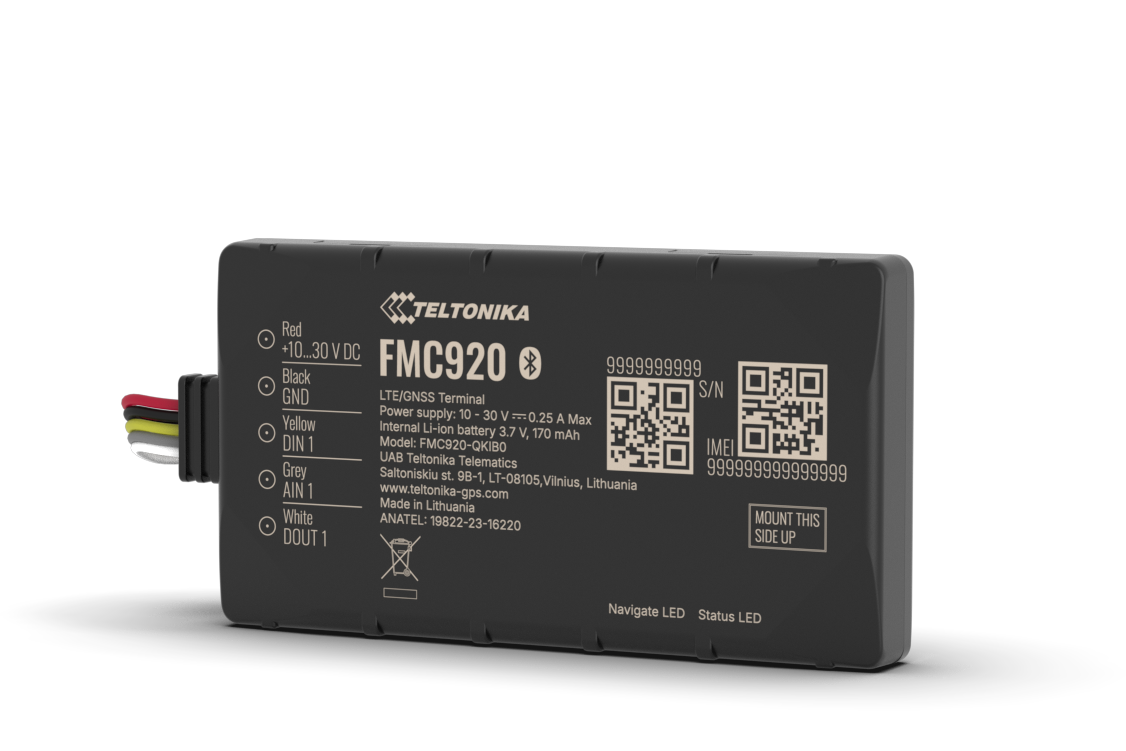
\includegraphics[width=0.14\linewidth,height=0.10\textheight,keepaspectratio]{./assets/result/market-devices/fmc920.png} & \textbf{Teltonika FMC920}~[10]\\Nhóm thiết bị nhỏ gọn & Phù hợp cho giám sát hành trình cơ bản, nhưng không theo dõi được thông số vận hành của xe. \\hline
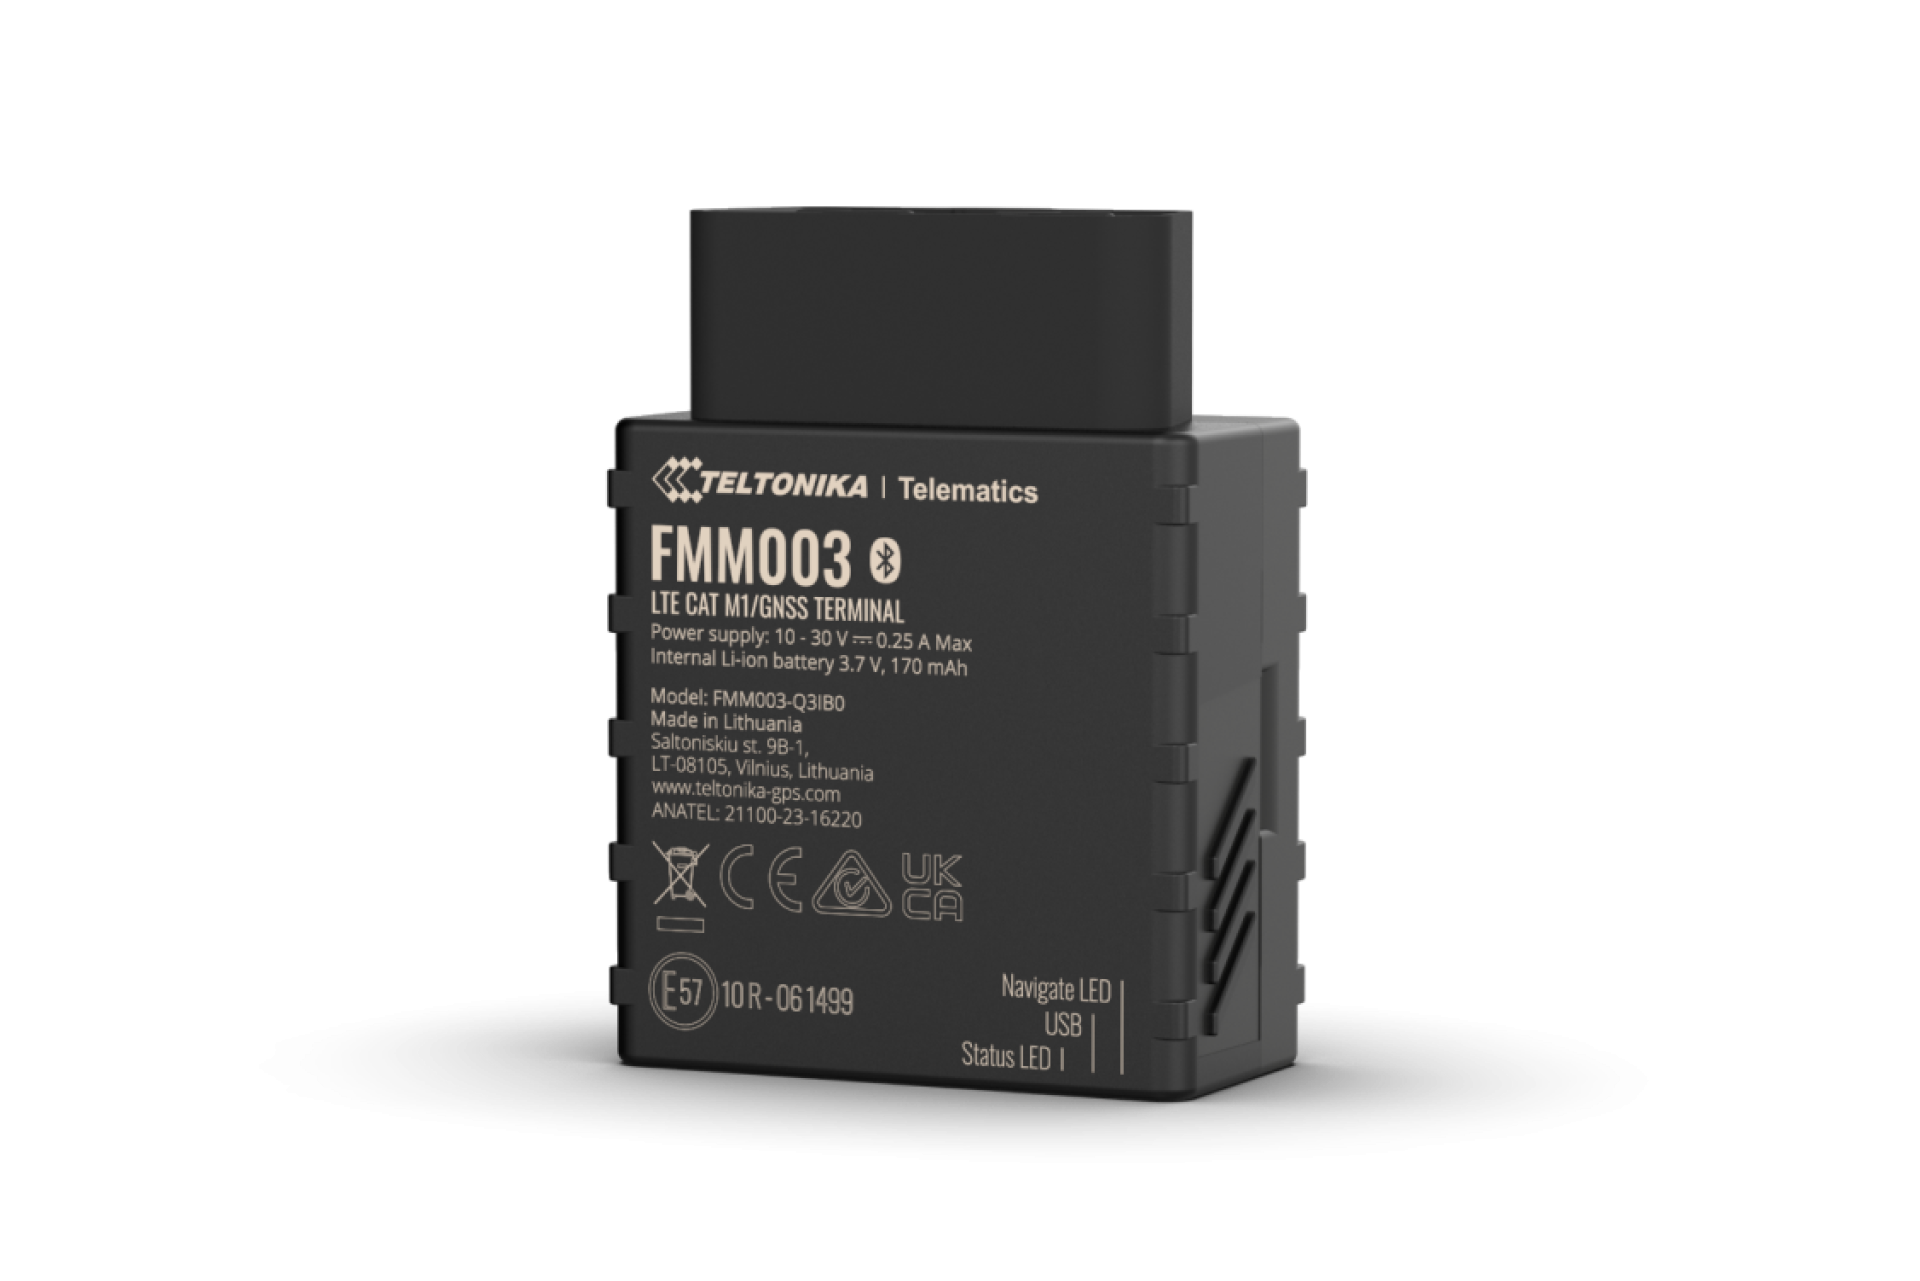
\includegraphics[width=0.14\linewidth,height=0.10\textheight,keepaspectratio]{./assets/result/market-devices/fmm003.png} & \textbf{Teltonika FMM003}~[11]\\Nhóm theo dõi được thông số vận hành & Cắm trực tiếp cổng OBD-II, phù hợp khi ưu tiên lắp đặt nhanh và lấy dữ liệu OBD-II cơ bản. \\hline
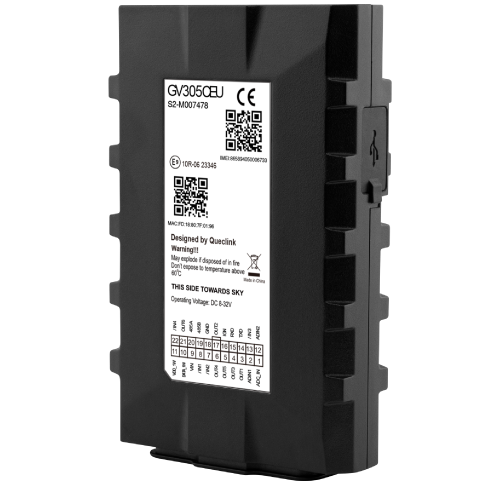
\includegraphics[width=0.14\linewidth,height=0.10\textheight,keepaspectratio]{./assets/result/market-devices/gv305ceu.png} & \textbf{Queclink GV305CEU}~[12]\\Nhóm thiết bị có nhiều giao tiếp mở rộng & Hỗ trợ nhiều giao tiếp mở rộng; phù hợp cho theo dõi dữ liệu mở rộng, nhưng thường vượt nhu cầu tối thiểu của đồ án. \\hline
\end{longtable}
}

Để làm rõ hạn chế đó, sinh viên tiến hành phân loại và so sánh các hướng triển khai
phổ biến dựa trên bốn tiêu chí kỹ thuật chính: mức độ dữ liệu thu được, khả năng lắp
đặt thực tế, mức độ hoàn chỉnh của hệ thống và chi phí triển khai.

\textbf{Bảng 2.3: So sánh các hướng triển khai giám sát xe hiện có}

{\def\LTcaptype{none} % do not increment counter
\begin{longtable}[]{@{}
  >{\raggedright\arraybackslash}p{(\linewidth - 6\tabcolsep) * \real{0.1573}}
  >{\raggedright\arraybackslash}p{(\linewidth - 6\tabcolsep) * \real{0.1973}}
  >{\raggedright\arraybackslash}p{(\linewidth - 6\tabcolsep) * \real{0.2800}}
  >{\raggedright\arraybackslash}p{(\linewidth - 6\tabcolsep) * \real{0.3653}}@{}}
\toprule\noalign{}
\begin{minipage}[b]{\linewidth}\raggedright
Hướng triển khai
\end{minipage} & \begin{minipage}[b]{\linewidth}\raggedright
Dữ liệu thu được
\end{minipage} & \begin{minipage}[b]{\linewidth}\raggedright
Ưu điểm kỹ thuật
\end{minipage} & \begin{minipage}[b]{\linewidth}\raggedright
Hạn chế chính
\end{minipage} \\
\midrule\noalign{}
\endhead
\bottomrule\noalign{}
\endlastfoot
Thiết bị định vị cơ bản & Vị trí, tốc độ, trạng thái kết nối & Lắp nhanh, cấu hình gọn, chi phí đầu tư thấp & Chỉ phù hợp cho giám sát hành trình cơ bản, thiếu dữ liệu vận hành và khó nhận biết bất thường khi xe đã tắt máy \\
Thiết bị định vị có khai thác dữ liệu chẩn đoán & Vị trí và một phần trạng thái vận hành của xe & Có thêm dữ liệu phục vụ giám sát khai thác, thuận lợi hơn cho việc đối chiếu sử dụng xe & Khả năng tập trung quản lý hạn chế, dữ liệu thường chưa đủ sâu và khả năng tùy biến hạn chế \\
Nền tảng quản lý đội xe thương mại & Vị trí, hành trình, cảnh báo, báo cáo, quản trị tập trung & Hệ thống hoàn chỉnh ở mức sản phẩm, triển khai nhanh, phù hợp quy mô lớn & Chi phí thuê bao và tích hợp cao, khó điều chỉnh theo nhu cầu kỹ thuật riêng của từng bài toán \\
Phương án tích hợp theo yêu cầu & Vị trí, dữ liệu vận hành, cảnh báo sự kiện, lịch sử khai thác & Linh hoạt theo mục tiêu quản lý, dễ mở rộng theo yêu cầu nghiên cứu và triển khai thực tế & Phải tự giải quyết đồng thời bài toán thiết bị, truyền dữ liệu, xử lý máy chủ và giao diện khai thác \\
\end{longtable}
}

Bảng 2.3 cho thấy khoảng trống kỹ thuật nằm ở nhóm giải pháp cần nhiều hơn một thiết
bị định vị đơn thuần, nhưng chưa cần tới một nền tảng thương mại có chi phí đầu tư và
vận hành cao. Đối với bài toán quản lý xe cho thuê quy mô nhỏ và vừa, hướng tiếp cận
phù hợp hơn là một hệ thống tích hợp vừa đủ: đủ dữ liệu để theo dõi hành trình, nhận
biết bất thường và đối chiếu khai thác, nhưng vẫn giữ được khả năng lắp đặt gọn và mở
rộng theo điều kiện triển khai thực tế.

Từ đó, cơ sở kỹ thuật của hệ thống được xác định theo ba điểm chính:

\begin{itemize}
\tightlist
\item
  dữ liệu vị trí, dữ liệu vận hành và dữ liệu sự kiện phải được xem là ba nguồn bổ sung cho nhau, không thể thay thế hoàn toàn cho nhau;
\item
  tuyến truyền dữ liệu phải phù hợp với đặc tính bản tin nhỏ, xuất hiện liên tục và có các mức ưu tiên khác nhau giữa dữ liệu nền và dữ liệu cảnh báo;
\item
  lớp xử lý và khai thác dữ liệu phải đủ rõ ràng để vừa phục vụ giám sát thời gian thực, vừa hỗ trợ tra cứu lịch sử và đối chiếu khai thác sau mỗi chuyến đi.
\end{itemize}

Các nhận định này là cơ sở để chuyển sang phần xác lập tiêu chí thiết kế ở Mục 2.3.

\subsection{2.3. Yêu cầu kỹ thuật và tiêu chuẩn thiết kế}\label{yuxeau-cux1ea7u-kux1ef9-thuux1eadt-vuxe0-tiuxeau-chuux1ea9n-thiux1ebft-kux1ebf}

Các yêu cầu kỹ thuật và ràng buộc thiết kế của hệ thống được trình bày tại Bảng 2.4 và
Bảng 2.5 như sau.

\textbf{Bảng 2.4: Chỉ tiêu thiết kế chính}

{\def\LTcaptype{none} % do not increment counter
\begin{longtable}[]{@{}
  >{\raggedright\arraybackslash}p{(\linewidth - 4\tabcolsep) * \real{0.1271}}
  >{\raggedright\arraybackslash}p{(\linewidth - 4\tabcolsep) * \real{0.4153}}
  >{\raggedright\arraybackslash}p{(\linewidth - 4\tabcolsep) * \real{0.4576}}@{}}
\toprule\noalign{}
\begin{minipage}[b]{\linewidth}\raggedright
Yếu tố thiết kế
\end{minipage} & \begin{minipage}[b]{\linewidth}\raggedright
Yêu cầu / giá trị
\end{minipage} & \begin{minipage}[b]{\linewidth}\raggedright
Ghi chú
\end{minipage} \\
\midrule\noalign{}
\endhead
\bottomrule\noalign{}
\endlastfoot
Nguồn cấp & 12-24 VDC & Phù hợp với hệ điện của phương tiện và là điều kiện nền cho việc lắp đặt trên xe thật \\
MCU điều khiển chính & Vi điều khiển họ ESP & Đáp ứng yêu cầu tích hợp truyền thông, đọc dữ liệu và điều khiển trạng thái năng lượng \\
Giao tiếp với phương tiện & Chuẩn OBD-II & Cho phép thu dữ liệu cơ bản phục vụ quản lý mà không đi theo hướng can thiệp điều khiển xe \\
Tham số quản lý chính & Tọa độ GPS, tốc độ hoạt động & Là các thông số tối thiểu để theo dõi hành trình và trạng thái sử dụng xe \\
Tính năng chính & Tính toán quãng đường, thời gian sử dụng, ước tính chi phí; Có cảnh báo hệ thống & Theo nhu cầu quản lý và khai thác \\
\end{longtable}
}

\textbf{Bảng 2.5: Ràng buộc thiết kế}

{\def\LTcaptype{none} % do not increment counter
\begin{longtable}[]{@{}
  >{\raggedright\arraybackslash}p{(\linewidth - 4\tabcolsep) * \real{0.1289}}
  >{\raggedright\arraybackslash}p{(\linewidth - 4\tabcolsep) * \real{0.2835}}
  >{\raggedright\arraybackslash}p{(\linewidth - 4\tabcolsep) * \real{0.5876}}@{}}
\toprule\noalign{}
\begin{minipage}[b]{\linewidth}\raggedright
Loại ràng buộc
\end{minipage} & \begin{minipage}[b]{\linewidth}\raggedright
Thông tin
\end{minipage} & \begin{minipage}[b]{\linewidth}\raggedright
Tác động đến thiết kế
\end{minipage} \\
\midrule\noalign{}
\endhead
\bottomrule\noalign{}
\endlastfoot
Tài chính & Tổng chi phí giải pháp không vượt 20.000.000 VND & Ưu tiên linh kiện phổ biến,~bảo đảm tính khả thi khi triển khai \\
Điều kiện kiểm chứng & Phòng thí nghiệm và xe thử nghiệm & Giải pháp phải đo kiểm được trên nguyên mẫu và đối chiếu được với điều kiện vận hành thực \\
Khả năng gia công & Mạch PCB, vỏ in 3D & Kết cấu phần cứng phải gọn, dễ chế tạo và phù hợp cho nguyên mẫu của đồ án \\
Tiêu chuẩn áp dụng & IPC-2221, IEC 60664-1 & Làm cơ sở cho bố trí mạch, khoảng cách cách điện và đánh giá an toàn điện ở mức nguyên mẫu \\
\end{longtable}
}

\subsection{2.4. Yêu cầu từ các bên liên quan}\label{yuxeau-cux1ea7u-tux1eeb-cuxe1c-buxean-liuxean-quan}

Bên cạnh tiêu chí kỹ thuật, bài toán còn chịu chi phối bởi cách các nhóm sử dụng và
vận hành hệ thống trên thực tế. Bảng 2.6 tổng hợp các yêu cầu chính và ảnh hưởng của
chúng đến thiết kế.

\textbf{Bảng 2.6: Yêu cầu từ các bên liên quan và tác động đến thiết kế}

{\def\LTcaptype{none} % do not increment counter
\begin{longtable}[]{@{}
  >{\raggedright\arraybackslash}p{(\linewidth - 4\tabcolsep) * \real{0.1489}}
  >{\raggedright\arraybackslash}p{(\linewidth - 4\tabcolsep) * \real{0.4298}}
  >{\raggedright\arraybackslash}p{(\linewidth - 4\tabcolsep) * \real{0.4213}}@{}}
\toprule\noalign{}
\begin{minipage}[b]{\linewidth}\raggedright
Bên liên quan
\end{minipage} & \begin{minipage}[b]{\linewidth}\raggedright
Nhu cầu chính
\end{minipage} & \begin{minipage}[b]{\linewidth}\raggedright
Ảnh hưởng tới thiết kế
\end{minipage} \\
\midrule\noalign{}
\endhead
\bottomrule\noalign{}
\endlastfoot
Đơn vị quản lý đội xe & Theo dõi vị trí, hành trình, cảnh báo và dữ liệu vận hành~xe trên cùng một hệ thống & Giao diện phải ưu tiên bản đồ quản lý, trạng thái, cảnh báo~và lịch sử chuyến đi \\
Người phụ trách kỹ thuật & Biết thiết bị nào online/offline, lỗi nguồn, lỗi mạng hoặc thiếu dữ liệu & Phải có lớp giám sát kỹ thuật tách khỏi lớp vận hành thường ngày \\
Đội lắp đặt/bảo trì & Lắp nhanh, ít xâm lấn, dễ thay xe và dễ khoanh vùng lỗi & Kết cấu phải gọn, kết nối rõ ràng, thao tác tháo lắp lặp lại được \\
Người lái hoặc người thuê xe & Thiết bị không ảnh hưởng tới vận hành xe và không thu thập vượt nhu cầu quản lý & Chức năng giám sát phải tách khỏi mọi hành vi điều khiển phương tiện \\
\end{longtable}
}

Điểm chung của các nhóm trên là đều cần thông tin rõ ràng, đủ để theo dõi và ra quyết
định, nhưng không làm tăng gánh nặng thao tác trong quá trình sử dụng. Vì vậy, các xử
lý kỹ thuật phức tạp nên được thực hiện ở lớp thiết bị và máy chủ; còn giao diện vận
hành chỉ nên tập trung vào các thông tin chính như vị trí, trạng thái và cảnh báo.

\chapterheading{CHƯƠNG 3. CÁC GIẢI PHÁP THIẾT KẾ - DESIGN SOLUTIONS}

\subsection{3.1. Phân tích tổng hợp}\label{phuxe2n-tuxedch-tux1ed5ng-hux1ee3p}

\subsubsection{3.1.1. Nguyên lý làm việc}\label{nguyuxean-luxfd-luxe0m-viux1ec7c}

Để đáp ứng yêu cầu giám sát phương tiện trong khai thác cho thuê xe tự lái, nguyên lý làm
việc của hệ thống có thể trình bày theo năm bước liên tiếp như sau:

\begin{itemize}
\tightlist
\item
  \textbf{Bước 1 - Ghi nhận trạng thái thực của xe:} Trên phương tiện tồn tại ba nhóm thông tin
  đầu vào chính gồm vị trí, dữ liệu vận hành và chuyển động. Đây là lớp thông tin phản ánh
  trực tiếp trạng thái vật lý của xe trong quá trình khai thác.
\item
  \textbf{Bước 2 - Thu nhận và xử lý tại thiết bị theo dõi:} Thiết bị trên xe tiếp nhận tín hiệu định vị
  từ GNSS, cổng chẩn đoán OBD-II và cảm biến gia tốc IMU, sau đó thực hiện tiền xử lý, chọn lọc và đóng gói dữ liệu. Nói
  cách khác, bản tin giám sát được hình thành ngay tại thiết bị chứ không phải ở mạng truyền dẫn.
\item
  \textbf{Bước 3 - Tạo và truyền bản tin giám sát:} Sau khi được đóng gói, dữ liệu được tổ chức
  thành bản tin giám sát định kỳ hoặc theo sự kiện và truyền về máy chủ qua mạng di động.
  Vai trò của kênh 4G/LTE trong giai đoạn này chỉ là mang bản tin đã tạo đi khỏi phương tiện.
\item
  \textbf{Bước 4 - Xử lý tại máy chủ:} Máy chủ tiếp nhận bản tin, thực hiện chuẩn hóa, lưu trữ,
  đối chiếu và phát hiện các trạng thái cần cảnh báo. Kết quả của bước này là lớp thông tin
  có thể dùng trực tiếp cho khai thác và theo dõi đội xe.
\item
  \textbf{Bước 5 - Biểu diễn thông tin quản lý:} Dữ liệu sau xử lý được đưa lên giao diện để hiển
  thị vị trí hiện thời, trạng thái hoạt động, lịch sử hành trình, dữ liệu chi tiết và các cảnh
  báo liên quan. Nhờ đó, người quản lý có thể theo dõi tập trung tình trạng phương tiện trên
  cùng một giao diện quản lý.
\end{itemize}

Theo cách tổ chức trên, hệ thống không chỉ dừng ở chức năng thu thập dữ liệu mà còn bảo đảm
quá trình chuyển hóa từ trạng thái thực của phương tiện thành thông tin có ý nghĩa quản lý.

\begin{figure}[H]
\centering
\pandocbounded{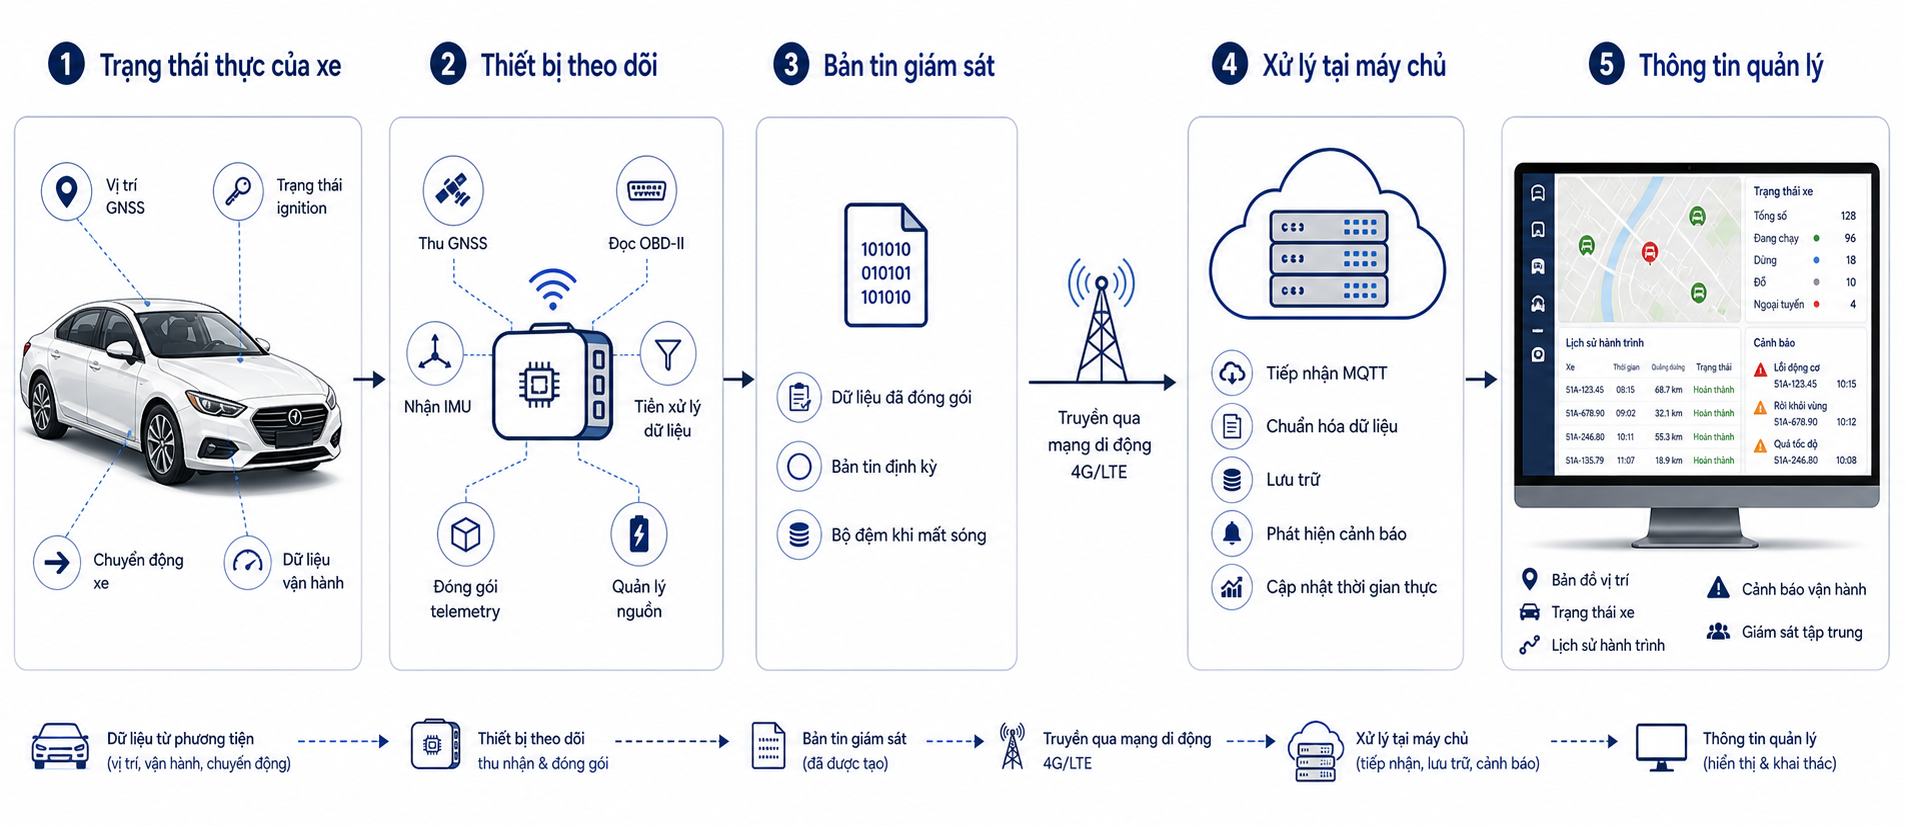
\includegraphics[keepaspectratio]{./assets/result/thesis-figure-3-1/hinh-3-1-nguyen-ly-chuyen-hoa-du-lieu-gpt-image.png}}
\caption*{Hình 3.1: Sơ đồ tổng thể của hệ thống thiết bị theo dõi}
\end{figure}

\emph{Hình 3.1: Nguyên lý chuyển hóa dữ liệu từ phương tiện thành thông tin quản lý}

\subsubsection{3.1.2. Các ràng buộc kỹ thuật chi phối phương án}\label{cuxe1c-ruxe0ng-buux1ed9c-kux1ef9-thuux1eadt-chi-phux1ed1i-phux1b0ux1a1ng-uxe1n}

Các ràng buộc kỹ thuật chi phối phương án thiết kế có thể quy về bốn nhóm chính như sau:

\begin{itemize}
\tightlist
\item
  \textbf{Ràng buộc ở lớp thiết bị:} Bộ theo dõi phải gọn, ít dây, dễ tháo lắp khi đổi xe, đồng
  thời không làm tăng mức can thiệp vào hệ điện hay ECU của xe. Vì vậy, khối điều khiển trung tâm,
  khối truyền dữ liệu - định vị và cách lấy dữ liệu OBD-II phải được cân nhắc cùng nhau.
\item
  \textbf{Ràng buộc về năng lượng:} Thiết bị bám vào ắc quy xe nên không được để dòng nền tích
  lũy thành mức hao điện đáng kể khi xe đỗ dài ngày. Tuy nhiên, hệ thống vẫn phải giữ được
  khả năng trở lại trạng thái hoạt động để phát hiện rung, dịch chuyển hoặc thay đổi trạng thái xe;
  do đó phần nguồn, cảm biến và cơ chế chuyển giữa hoạt động và ngủ sâu phải được xét như một
  cụm chung.
\item
  \textbf{Ràng buộc ở tuyến truyền dữ liệu:} Xe hoạt động trong điều kiện sóng thay đổi liên tục,
  nên phương án truyền không thể giả định kết nối luôn ổn định. Kiến trúc được chọn phải
  chấp nhận mất sóng cục bộ, có bộ nhớ đệm phù hợp và phục hồi được tuyến dữ liệu sau khi
  kết nối lại.
\item
  \textbf{Ràng buộc ở lớp khai thác thông tin:} Dữ liệu thu được có nhiều lớp, nhưng giao diện
  vận hành không thể trở thành nơi dồn mọi thứ. Phương án chỉ được xem là đạt khi phần phức
  tạp được giữ ở lớp thiết bị và lớp máy chủ, còn giao diện chỉ giữ những tín hiệu thực sự
  cần cho quyết định quản lý.
\end{itemize}

\subsection{3.2. Đề xuất các giải pháp}\label{ux111ux1ec1-xuux1ea5t-cuxe1c-giux1ea3i-phuxe1p}

\subsubsection{3.2.1. Đề xuất giải pháp phần cứng thiết bị}\label{ux111ux1ec1-xuux1ea5t-giux1ea3i-phuxe1p-phux1ea7n-cux1ee9ng-thiux1ebft-bux1ecb}

a, Phương án lấy dữ liệu từ cổng chẩn đoán OBD-II

Ở nhánh OBD-II, đồ án chỉ cần thu nhóm dữ liệu phục vụ quản lý nên không đi theo hướng chẩn
đoán sâu hay can thiệp nhiều vào xe. Từ yêu cầu đó, ba hướng khai thác được xét gồm ghép trực
tiếp vào tuyến OBD-II, dùng bộ chuyển đổi ELM327 có dây và dùng bộ chuyển đổi Bluetooth
\texttt{vgate\ iCar\ Pro}.

\textbf{Bảng 3.1: Ma trận đánh giá phương án thu dữ liệu OBD-II}

{\def\LTcaptype{none} % do not increment counter
\begin{longtable}[]{@{}
  >{\raggedright\arraybackslash}p{(\linewidth - 8\tabcolsep) * \real{0.4645}}
  >{\raggedright\arraybackslash}p{(\linewidth - 8\tabcolsep) * \real{0.0903}}
  >{\raggedright\arraybackslash}p{(\linewidth - 8\tabcolsep) * \real{0.2323}}
  >{\raggedright\arraybackslash}p{(\linewidth - 8\tabcolsep) * \real{0.0968}}
  >{\raggedright\arraybackslash}p{(\linewidth - 8\tabcolsep) * \real{0.1161}}@{}}
\toprule\noalign{}
\begin{minipage}[b]{\linewidth}\raggedright
Tiêu chí đánh giá
\end{minipage} & \begin{minipage}[b]{\linewidth}\raggedright
Trọng số (\%)
\end{minipage} & \begin{minipage}[b]{\linewidth}\raggedright
Ghép trực tiếp vào tuyến OBD-II
\end{minipage} & \begin{minipage}[b]{\linewidth}\raggedright
ELM327 có dây
\end{minipage} & \begin{minipage}[b]{\linewidth}\raggedright
\texttt{vgate\ iCar\ Pro}
\end{minipage} \\
\midrule\noalign{}
\endhead
\bottomrule\noalign{}
\endlastfoot
Mức xâm lấn lên hệ điện và khả năng trả xe về nguyên trạng & 35 & 1 & 3 & 5 \\
Khả năng tương thích giao thức trên nhiều dòng xe & 30 & 1 & 3 & 5 \\
Thuận tiện khi tháo lắp, chuyển xe và khoanh vùng lỗi & 20 & 1 & 2 & 5 \\
Mức đáp ứng nhóm tham số quản lý cần theo dõi & 15 & 5 & 4 & 4 \\
\textbf{Tổng điểm quy đổi} & \textbf{100} & \textbf{1,60} & \textbf{3,00} & \textbf{4,85} \\
\end{longtable}
}

Kết quả ở Bảng 3.1 cho thấy \texttt{vgate\ iCar\ Pro} phù hợp hơn hai phương án còn lại. Phương án
này vẫn giữ được nhóm dữ liệu cần thiết, nhưng ít xâm lấn hơn và thuận tiện hơn khi đội xe có nhiều loại xe khác nhau.

\begin{figure}[H]
\centering
\pandocbounded{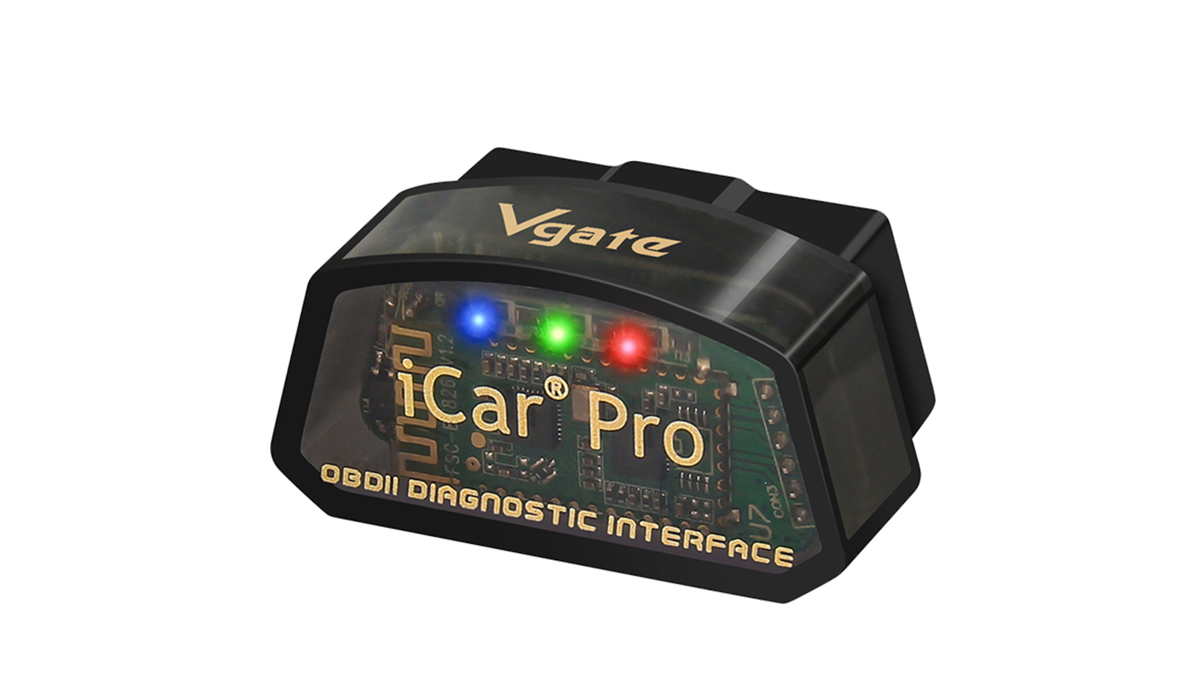
\includegraphics[keepaspectratio]{./assets/result/chapter-3-selected-components/hinh-3-2-vgate-icar-pro-ble.png}}
\caption*{Hình 3.2: Bộ đọc OBD-II vgate iCar Pro BLE}
\end{figure}

\emph{Hình 3.2: Bộ đọc OBD-II Bluetooth vgate iCar Pro được chọn cho nhánh thu dữ liệu vận hành}

b, Phương án duy trì giám sát khi xe đỗ

Khi khóa điện tắt, thiết bị không nên duy trì toàn bộ hoạt động (modem 4G, GNSS và OBD-II) như lúc xe
đang hoạt động; nhưng cũng không thể tắt hẳn vì vẫn cần nhận biết rung hoặc dịch chuyển
bất thường. Vì vậy, phương án ở nhánh này được xét như một cặp: phần tử đánh thức tiêu
thụ thấp và cách cấp nguồn cho các khối còn lại. Nguồn chung là cách cấp cùng một nhánh
cho phần giám sát và các tải lớn; nguồn theo khóa điện chỉ còn nguồn khi xe bật khóa và
mất nguồn khi xe tắt khóa; còn nguồn chia nhánh giữ một nhánh nhỏ luôn cấp cho đánh thức,
trong khi modem, GNSS và OBD-II được đóng cắt riêng.

\textbf{Bảng 3.2: Ma trận đánh giá phương án duy trì giám sát khi xe đỗ}

{\def\LTcaptype{none} % do not increment counter
\begin{longtable}[]{@{}
  >{\raggedright\arraybackslash}p{(\linewidth - 8\tabcolsep) * \real{0.4272}}
  >{\raggedright\arraybackslash}p{(\linewidth - 8\tabcolsep) * \real{0.0680}}
  >{\raggedright\arraybackslash}p{(\linewidth - 8\tabcolsep) * \real{0.1748}}
  >{\raggedright\arraybackslash}p{(\linewidth - 8\tabcolsep) * \real{0.1553}}
  >{\raggedright\arraybackslash}p{(\linewidth - 8\tabcolsep) * \real{0.1748}}@{}}
\toprule\noalign{}
\begin{minipage}[b]{\linewidth}\raggedright
Tiêu chí đánh giá
\end{minipage} & \begin{minipage}[b]{\linewidth}\raggedright
Trọng số (\%)
\end{minipage} & \begin{minipage}[b]{\linewidth}\raggedright
SW-420 + cấp chung toàn thiết bị
\end{minipage} & \begin{minipage}[b]{\linewidth}\raggedright
MPU6050 + cấp theo khóa điện
\end{minipage} & \begin{minipage}[b]{\linewidth}\raggedright
LIS3DSH + nhánh đánh thức riêng
\end{minipage} \\
\midrule\noalign{}
\endhead
\bottomrule\noalign{}
\endlastfoot
Mức tiêu thụ khi chỉ giữ giám sát trong thời gian xe đỗ & 35 & 2 & 2 & 5 \\
Khả năng đánh thức thiết bị bằng chuyển động khi MCU và modem đã ngủ sâu & 25 & 2 & 4 & 4 \\
Khả năng tách modem, GNSS và OBD-II khỏi nhánh luôn cấp & 25 & 1 & 2 & 5 \\
Mức an toàn với ắc quy và độ ổn định khi modem phát dòng xung & 15 & 2 & 3 & 5 \\
\textbf{Tổng điểm quy đổi} & \textbf{100} & \textbf{1,75} & \textbf{2,65} & \textbf{4,75} \\
\end{longtable}
}

Theo Bảng 3.2, LIS3DSH kết hợp nhánh đánh thức riêng phù hợp hơn cho trạng thái xe đỗ. Phương
án này giữ lại đường đánh thức tiêu thụ thấp, đồng thời cho phép đưa phần lớn thiết bị về
ngủ sâu và cô lập nhánh modem khỏi nguồn logic khi có xung dòng lớn.

\begin{figure}[H]
\centering
\pandocbounded{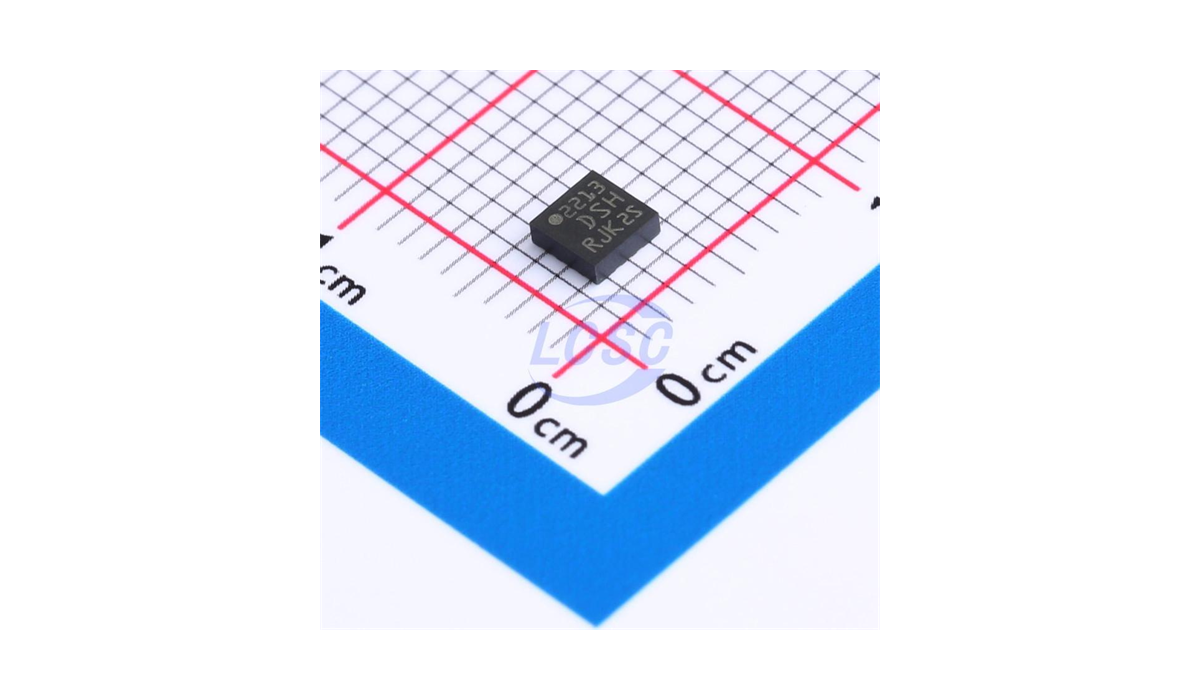
\includegraphics[keepaspectratio]{./assets/result/chapter-3-selected-components/hinh-3-3-lis3dsh-mat-truoc-lcsc-front.png}}
\caption*{Hình 3.3: Cảm biến gia tốc LIS3DSH}
\end{figure}

\emph{Hình 3.3: Cảm biến gia tốc LIS3DSH được chọn cho nhánh phát hiện chuyển động khi xe đỗ}

c, Phương án truyền dữ liệu và định vị

Ở tuyến truyền dữ liệu và định vị, thiết bị chỉ gửi các bản tin nhỏ như vị trí, trạng thái
và cảnh báo; do đó vấn đề chính không phải là tốc độ truyền cực đại. Điều cần cân nhắc là
cách ghép khối truyền dữ liệu di động với khối định vị sao cho ít khối phải điều khiển, nguồn
ổn định và phù hợp với không gian lắp trong xe. Các mô-đun chỉ hỗ trợ 2G không được đưa vào
so sánh vì không còn phù hợp với điều kiện mạng di động tại Việt Nam {[}13{]}. Ba phương án đại diện
được xét gồm:

\begin{enumerate}
\def\labelenumi{\arabic{enumi}.}
\tightlist
\item
  \textbf{EC200U-CN + L76K:} EC200U-CN đảm nhiệm truyền dữ liệu LTE Cat 1, còn L76K là mô-đun
  GNSS rời. Cách này dùng được mạng 4G hiện nay, nhưng thiết bị vẫn phải điều khiển riêng
  khối truyền dữ liệu và khối định vị.
\item
  \textbf{A7670C + ATGM336H:} A7670C đảm nhiệm truyền dữ liệu LTE, ATGM336H đảm nhiệm định vị
  GNSS. Phương án này cũng đi theo hướng 4G, nhưng phần định vị vẫn tách thành một khối riêng.
\item
  \textbf{SIM7600CE-T:} Mô-đun này tích hợp LTE và GNSS trong cùng một khối, giúp gom phần truyền
  dữ liệu và định vị về cùng một đường điều khiển.
\end{enumerate}

\textbf{Bảng 3.3: Ma trận đánh giá phương án truyền dữ liệu và định vị}

{\def\LTcaptype{none} % do not increment counter
\begin{longtable}[]{@{}
  >{\raggedright\arraybackslash}p{(\linewidth - 8\tabcolsep) * \real{0.5563}}
  >{\raggedright\arraybackslash}p{(\linewidth - 8\tabcolsep) * \real{0.0927}}
  >{\raggedright\arraybackslash}p{(\linewidth - 8\tabcolsep) * \real{0.1060}}
  >{\raggedright\arraybackslash}p{(\linewidth - 8\tabcolsep) * \real{0.1126}}
  >{\raggedright\arraybackslash}p{(\linewidth - 8\tabcolsep) * \real{0.1325}}@{}}
\toprule\noalign{}
\begin{minipage}[b]{\linewidth}\raggedright
Tiêu chí đánh giá
\end{minipage} & \begin{minipage}[b]{\linewidth}\raggedright
Trọng số (\%)
\end{minipage} & \begin{minipage}[b]{\linewidth}\raggedright
EC200U-CN + L76K
\end{minipage} & \begin{minipage}[b]{\linewidth}\raggedright
A7670C + ATGM336H
\end{minipage} & \begin{minipage}[b]{\linewidth}\raggedright
SIM7600CE-T LTE/GNSS
\end{minipage} \\
\midrule\noalign{}
\endhead
\bottomrule\noalign{}
\endlastfoot
Số khối phải khởi tạo và giám sát cho truyền dữ liệu và định vị & 30 & 2 & 2 & 5 \\
Độ phức tạp của nguồn, mạch vô tuyến và bố trí ăng ten trên thiết bị & 30 & 3 & 3 & 5 \\
Khả năng giữ và khôi phục đường truyền, vị trí khi xe di động & 25 & 4 & 4 & 4 \\
Mức phù hợp với không gian lắp trên xe và vỏ thiết bị & 15 & 3 & 3 & 5 \\
\textbf{Tổng điểm quy đổi} & \textbf{100} & \textbf{2,95} & \textbf{3,00} & \textbf{4,75} \\
\end{longtable}
}

Theo Bảng 3.3, SIM7600CE-T là phương án phù hợp hơn trong nhóm so sánh. Lợi thế cốt lõi
của mô-đun này là gom đường truyền dữ liệu và định vị về một khối thống nhất, từ đó giảm
rõ phần nguồn, ăng ten và trình tự khởi tạo phải xử lý trên thiết bị.

\begin{figure}[H]
\centering
\pandocbounded{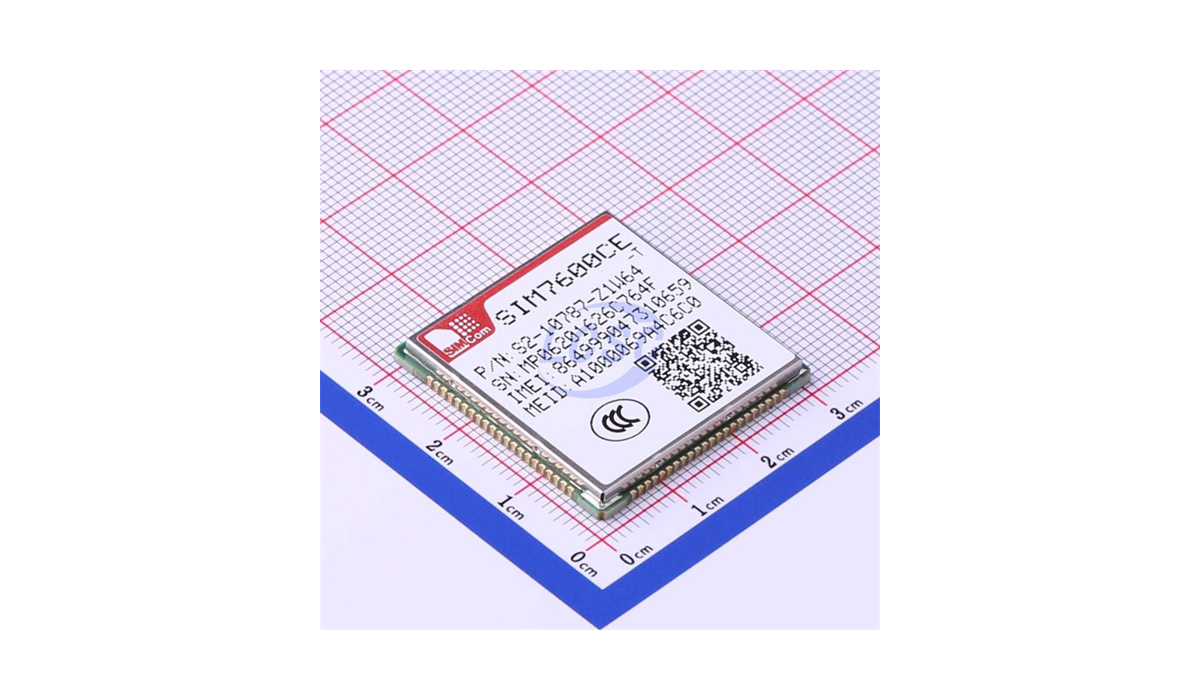
\includegraphics[keepaspectratio]{./assets/result/chapter-3-selected-components/hinh-3-4-sim7600ce-t.png}}
\caption*{Hình 3.4: Mô-đun SIM7600CE-T}
\end{figure}

\emph{Hình 3.4: Mô-đun SIM7600CE-T tích hợp LTE và GNSS được chọn cho tuyến truyền dữ liệu - định vị}

d, Phương án bộ điều khiển trung tâm

Bộ điều khiển trung tâm là khối điều phối các phần đã chọn ở trên: modem LTE/GNSS, kết nối
OBD-II không dây, cảm biến đánh thức, bộ nhớ đệm và cổng bảo trì. Vì vậy, phương án MCU không
chỉ được xét theo năng lực xử lý, mà chủ yếu theo số giao tiếp còn đủ, mức tích hợp không dây,
khả năng ngủ sâu và lượng phần cứng phụ phải ghép thêm. Ba hướng đại diện được đưa vào so sánh
gồm ESP32-S3, STM32L4 ghép Bluetooth rời và nRF52840.

\textbf{Bảng 3.4: Ma trận đánh giá phương án bộ điều khiển trung tâm}

{\def\LTcaptype{none} % do not increment counter
\begin{longtable}[]{@{}
  >{\raggedright\arraybackslash}p{(\linewidth - 8\tabcolsep) * \real{0.6048}}
  >{\raggedright\arraybackslash}p{(\linewidth - 8\tabcolsep) * \real{0.0838}}
  >{\raggedright\arraybackslash}p{(\linewidth - 8\tabcolsep) * \real{0.0838}}
  >{\raggedright\arraybackslash}p{(\linewidth - 8\tabcolsep) * \real{0.1437}}
  >{\raggedright\arraybackslash}p{(\linewidth - 8\tabcolsep) * \real{0.0838}}@{}}
\toprule\noalign{}
\begin{minipage}[b]{\linewidth}\raggedright
Tiêu chí đánh giá
\end{minipage} & \begin{minipage}[b]{\linewidth}\raggedright
Trọng số (\%)
\end{minipage} & \begin{minipage}[b]{\linewidth}\raggedright
ESP32-S3
\end{minipage} & \begin{minipage}[b]{\linewidth}\raggedright
STM32L4 + Bluetooth rời
\end{minipage} & \begin{minipage}[b]{\linewidth}\raggedright
nRF52840
\end{minipage} \\
\midrule\noalign{}
\endhead
\bottomrule\noalign{}
\endlastfoot
Khả năng giữ đồng thời các giao tiếp cho modem, BLE OBD-II, IMU và cổng bảo trì & 35 & 5 & 4 & 3 \\
Phần nhớ và tài nguyên còn lại cho lưu đệm bản tin, nhật ký lỗi và cập nhật firmware & 25 & 4 & 3 & 2 \\
Khả năng vào ngủ sâu và đánh thức bằng tín hiệu ngoài & 20 & 4 & 5 & 4 \\
Mức phải ghép thêm chip vô tuyến và mạch phụ trợ & 20 & 5 & 2 & 3 \\
\textbf{Tổng điểm quy đổi} & \textbf{100} & \textbf{4,55} & \textbf{3,55} & \textbf{2,95} \\
\end{longtable}
}

Từ Bảng 3.4, ESP32-S3 là phương án phù hợp hơn trong nhóm so sánh. Điểm quyết định của
lựa chọn này là giữ được đủ giao tiếp cho toàn bộ thiết bị mà không phải hy sinh tài nguyên
cho một khối Bluetooth rời.

\begin{figure}[H]
\centering
\pandocbounded{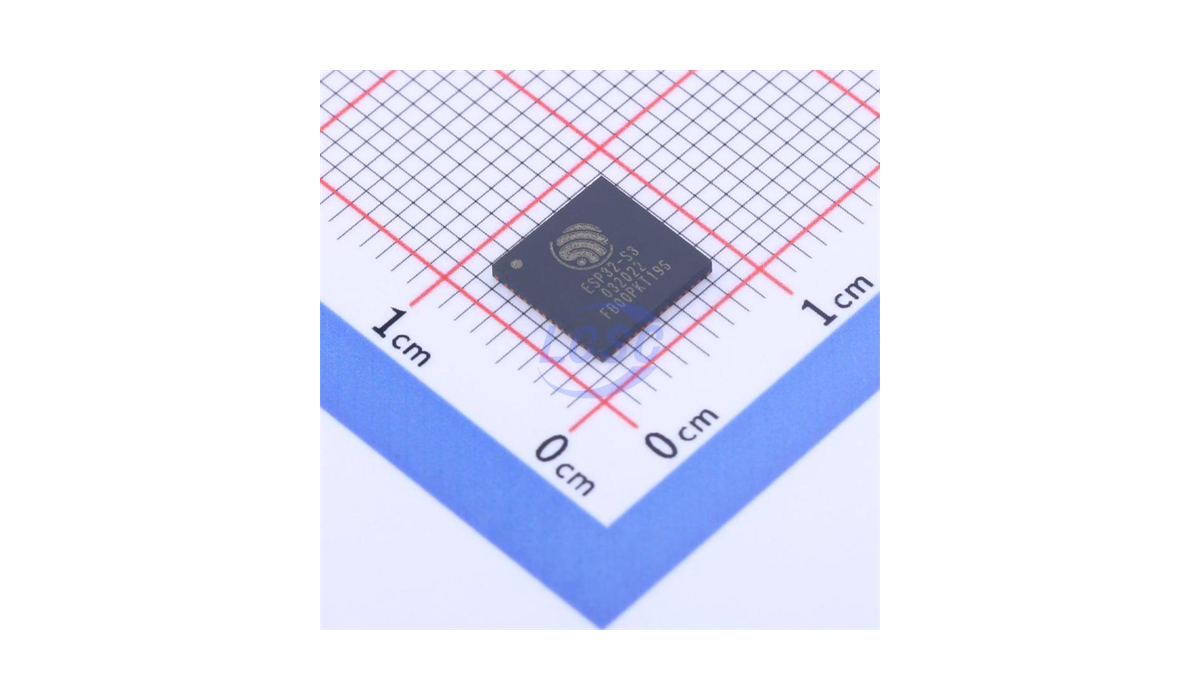
\includegraphics[keepaspectratio]{./assets/result/chapter-3-selected-components/hinh-3-5-esp32-s3-chip-lcsc-front.png}}
\caption*{Hình 3.5: Chip ESP32-S3}
\end{figure}

\emph{Hình 3.5: Chip ESP32-S3 được chọn làm bộ điều khiển trung tâm của thiết bị}

\subsubsection{3.2.2. Đề xuất giải pháp phần mềm nhúng}\label{ux111ux1ec1-xuux1ea5t-giux1ea3i-phuxe1p-phux1ea7n-mux1ec1m-nhuxfang}

Ở lớp phần mềm nhúng, vấn đề cần xác định trước hết là nền tảng phát triển và cách tổ chức
thực thi trên ESP32-S3. Thiết bị phải đồng thời làm việc với modem LTE/GNSS, kết nối BLE tới
bộ đọc OBD-II, lưu đệm cục bộ và giữ khả năng mở rộng cho bảo trì sau này. Vì vậy, ở bước
đề xuất giải pháp, phần mềm nhúng được xét theo ba hướng sau:

\begin{enumerate}
\def\labelenumi{\arabic{enumi}.}
\tightlist
\item
  \textbf{Arduino core trên ESP32:} Cách này thuận tiện khi dựng nguyên mẫu nhanh, thư viện phong
  phú và dễ tiếp cận, nhưng việc kiểm soát tài nguyên, tác vụ nền và mở rộng hệ thống dài hạn
  không phải là điểm mạnh.
\item
  \textbf{ESP-IDF theo vòng lặp chính:} Hướng này bám sát SDK chính thức của hãng Espressif, giúp kiểm
  soát phần cứng tốt hơn và khai thác đầy đủ driver hệ thống, nhưng khi số khối ngoại vi tăng lên
  thì việc dồn phần lớn xử lý vào một luồng chính sẽ sớm chật.
\item
  \textbf{ESP-IDF kết hợp FreeRTOS:} Đây là hướng dùng SDK chính thức đồng thời tổ chức các tác vụ
  theo cơ chế thời gian thực, phù hợp hơn khi thiết bị phải ghép nhiều nhánh xử lý có nhịp làm việc khác nhau.
\end{enumerate}

Các phương án được so sánh theo bốn tiêu chí: mức phù hợp khi tích hợp nhiều khối ngoại vi,
khả năng kiểm soát tài nguyên và tác vụ nền, thuận lợi cho bảo trì - mở rộng firmware, và mức
dựa vào nền tảng chính thức của nhà sản xuất.

\textbf{Bảng 3.5: Ma trận đánh giá phương án phần mềm nhúng trên thiết bị}

{\def\LTcaptype{none} % do not increment counter
\begin{longtable}[]{@{}
  >{\raggedright\arraybackslash}p{(\linewidth - 8\tabcolsep) * \real{0.5196}}
  >{\raggedright\arraybackslash}p{(\linewidth - 8\tabcolsep) * \real{0.0782}}
  >{\raggedright\arraybackslash}p{(\linewidth - 8\tabcolsep) * \real{0.1341}}
  >{\raggedright\arraybackslash}p{(\linewidth - 8\tabcolsep) * \real{0.1676}}
  >{\raggedright\arraybackslash}p{(\linewidth - 8\tabcolsep) * \real{0.1006}}@{}}
\toprule\noalign{}
\begin{minipage}[b]{\linewidth}\raggedright
Tiêu chí đánh giá
\end{minipage} & \begin{minipage}[b]{\linewidth}\raggedright
Trọng số (\%)
\end{minipage} & \begin{minipage}[b]{\linewidth}\raggedright
Arduino core trên ESP32
\end{minipage} & \begin{minipage}[b]{\linewidth}\raggedright
ESP-IDF theo vòng lặp chính
\end{minipage} & \begin{minipage}[b]{\linewidth}\raggedright
ESP-IDF + FreeRTOS
\end{minipage} \\
\midrule\noalign{}
\endhead
\bottomrule\noalign{}
\endlastfoot
Mức phù hợp khi tích hợp đồng thời modem, BLE OBD-II, lưu đệm và nhánh bảo trì & 35 & 3 & 4 & 5 \\
Khả năng kiểm soát tài nguyên, tác vụ nền và nhịp xử lý của hệ thống & 25 & 2 & 3 & 5 \\
Thuận lợi cho bảo trì, mở rộng và tổ chức lại firmware khi hệ thống lớn dần & 25 & 3 & 4 & 5 \\
Mức bám sát nền tảng chính thức của Espressif & 15 & 2 & 5 & 5 \\
\textbf{Tổng điểm quy đổi} & \textbf{100} & \textbf{2,70} & \textbf{4,00} & \textbf{5,00} \\
\end{longtable}
}

Từ Bảng 3.5, hướng ESP-IDF kết hợp FreeRTOS có điểm cao nhất nên được giữ lại. Điểm mạnh
của phương án này là vừa bám SDK chính thức của Espressif, vừa thuận lợi hơn khi thiết bị
phải điều phối nhiều khối ngoại vi trong cùng một phần mềm nhúng (firmware).

\subsubsection{3.2.3. Đề xuất giải pháp truyền bản tin và định hướng tổ chức phía máy chủ}\label{ux111ux1ec1-xuux1ea5t-giux1ea3i-phuxe1p-truyux1ec1n-bux1ea3n-tin-vuxe0-ux111ux1ecbnh-hux1b0ux1edbng-tux1ed5-chux1ee9c-phuxeda-muxe1y-chux1ee7}

Ở lớp truyền dữ liệu, bước đầu tiên là chọn kênh đưa bản tin từ thiết bị lên máy chủ. Dữ liệu của hệ
thống chủ yếu là các gói tin nhỏ, phát sinh theo chu kỳ hoặc theo sự kiện, đi qua mạng di động
và có thể bị gián đoạn. Vì vậy, giao thức được chọn phải đủ nhẹ cho thiết bị, dễ tách nhóm dữ
liệu và hỗ trợ tốt cho tình huống mất sóng rồi gửi bù. Ba hướng được xét gồm:

\begin{itemize}
\item
  \textbf{HTTPS/REST - giao thức gửi yêu cầu tới API (Application Programming Interface - giao diện lập trình ứng dụng) của máy chủ}

  \begin{itemize}
  \tightlist
  \item
    Cách này cho thiết bị gửi từng yêu cầu riêng lên API của máy chủ; máy chủ nhận xong thì trả phản
    hồi và kết thúc phiên trao đổi. Về bản chất, mỗi bản tin dữ liệu tương ứng với một lần yêu cầu -
    phản hồi riêng biệt giữa thiết bị và máy chủ.
  \item
    Ưu điểm là quen thuộc, dễ lập trình và dễ kiểm thử bằng các công cụ web thông dụng.
  \item
    Hạn chế là khi dữ liệu phát sinh lặp lại theo chu kỳ ngắn, việc phải mở và đóng nhiều phiên trao
    đổi làm tuyến truyền nặng hơn mức cần thiết.
  \end{itemize}
\item
  \textbf{WebSocket/TCP - cơ chế duy trì kết nối liên tục giữa thiết bị và máy chủ}

  \begin{itemize}
  \tightlist
  \item
    Cách này cho thiết bị tạo một kết nối liên tục với máy chủ và giữ kết nối đó trong suốt thời gian
    làm việc, nên dữ liệu có thể đi hai chiều trên cùng một đường truyền. Về bản chất, thiết bị và
    máy chủ duy trì một phiên kết nối kéo dài để trao đổi dữ liệu liên tục.
  \item
    Ưu điểm là thuận lợi khi cần cập nhật liên tục.
  \item
    Hạn chế là phụ thuộc nhiều vào việc kết nối phải được giữ ổn định, trong khi thiết bị có thể đi
    vào ngủ sâu hoặc di chuyển qua vùng sóng yếu.
  \end{itemize}
\item
  \textbf{MQTT qua TLS - giao thức bản tin nhẹ có mã hóa đường truyền}

  \begin{itemize}
  \tightlist
  \item
    Cách này không gửi dữ liệu thẳng vào một API cố định mà đưa từng bản tin lên các kênh chủ đề; phía
    máy chủ sẽ đăng ký nhận theo từng nhóm chủ đề tương ứng. Về bản chất, bản tin được phân loại theo
    từng chủ đề ngay từ khi phát đi, nhờ đó phía nhận chỉ cần xử lý đúng nhóm dữ liệu liên quan.
  \item
    \texttt{MQTT} (Message Queuing Telemetry Transport - giao thức truyền bản tin nhẹ) được thiết kế cho bản
    tin nhỏ và thiết bị tài nguyên hạn chế, còn \texttt{TLS} (Transport Layer Security - giao thức bảo mật lớp
    truyền tải) là lớp mã hóa bổ sung để bảo vệ dữ liệu khi truyền qua mạng di động công cộng.
  \item
    Vì vậy, hướng này gọn hơn cho bài toán giám sát lặp lại và thuận lợi hơn khi cần tách riêng dữ liệu
    vị trí, trạng thái và cảnh báo.
  \end{itemize}
\end{itemize}

\textbf{Bảng 3.6: Ma trận đánh giá giao thức truyền bản tin từ thiết bị}

{\def\LTcaptype{none} % do not increment counter
\begin{longtable}[]{@{}
  >{\raggedright\arraybackslash}p{(\linewidth - 8\tabcolsep) * \real{0.6028}}
  >{\raggedright\arraybackslash}p{(\linewidth - 8\tabcolsep) * \real{0.0993}}
  >{\raggedright\arraybackslash}p{(\linewidth - 8\tabcolsep) * \real{0.0993}}
  >{\raggedright\arraybackslash}p{(\linewidth - 8\tabcolsep) * \real{0.0993}}
  >{\raggedright\arraybackslash}p{(\linewidth - 8\tabcolsep) * \real{0.0993}}@{}}
\toprule\noalign{}
\begin{minipage}[b]{\linewidth}\raggedright
Tiêu chí đánh giá
\end{minipage} & \begin{minipage}[b]{\linewidth}\raggedright
Trọng số (\%)
\end{minipage} & \begin{minipage}[b]{\linewidth}\raggedright
HTTPS/REST
\end{minipage} & \begin{minipage}[b]{\linewidth}\raggedright
WebSocket/TCP
\end{minipage} & \begin{minipage}[b]{\linewidth}\raggedright
MQTT qua TLS
\end{minipage} \\
\midrule\noalign{}
\endhead
\bottomrule\noalign{}
\endlastfoot
Phù hợp với bản tin nhỏ, gửi định kỳ hoặc theo sự kiện & 30 & 3 & 4 & 5 \\
Mức nhẹ cho thiết bị và modem khi truyền qua mạng di động & 25 & 3 & 3 & 5 \\
Khả năng phân tách dữ liệu vị trí, trạng thái và cảnh báo theo chủ đề & 25 & 2 & 3 & 5 \\
Thuận lợi cho gửi lại, gửi bù sau gián đoạn kết nối & 20 & 3 & 2 & 4 \\
\textbf{Tổng điểm quy đổi} & \textbf{100} & \textbf{2,75} & \textbf{3,10} & \textbf{4,80} \\
\end{longtable}
}

Từ Bảng 3.6, \texttt{MQTT\ qua\ TLS} được chọn làm giao thức truyền bản tin chính từ thiết bị lên máy chủ,
vì phù hợp hơn với đặc điểm dữ liệu nhỏ, phát sinh lặp lại và có thể bị gián đoạn theo chất lượng
mạng di động. Trong khi đó, \texttt{HTTPS/REST} vẫn phù hợp cho các API cấu hình, quản trị hoặc trao đổi
giữa giao diện và \texttt{backend} (lớp xử lý nghiệp vụ phía máy chủ), nhưng không phải kênh chính cho luồng
dữ liệu giám sát phát sinh liên tục từ thiết bị.

Khi giao thức truyền bản tin đã được xác định, vấn đề tiếp theo là cách tổ chức phần máy chủ để tiếp
nhận, xử lý và lưu trữ dữ liệu. Ba hướng chính được xem xét gồm:

\begin{itemize}
\item
  \textbf{Backend (lớp xử lý nghiệp vụ phía máy chủ) nhận và xử lý trực tiếp - một ứng dụng duy nhất đảm nhiệm toàn bộ tuyến dữ liệu}

  \begin{itemize}
  \tightlist
  \item
    Cách này gom phần nhận bản tin, xử lý nghiệp vụ và lưu trữ vào cùng một ứng dụng.
  \item
    Về bản chất, toàn bộ tuyến xử lý dữ liệu được đặt trong một khối chức năng duy nhất.
  \item
    Ưu điểm là số lượng dịch vụ ít, cấu trúc ban đầu tương đối đơn giản.
  \item
    Hạn chế là khi khối lượng dữ liệu tăng lên, phần tiếp nhận bản tin và phần nghiệp vụ dễ ảnh hưởng
    lẫn nhau, đồng thời việc mở rộng hoặc khoanh vùng lỗi cũng kém thuận lợi hơn.
  \end{itemize}
\item
  \textbf{MQTT broker (lớp tiếp nhận và phân phối bản tin) + backend xử lý tập trung - tách lớp nhận bản tin nhưng vẫn dồn xử lý vào backend}

  \begin{itemize}
  \tightlist
  \item
    Cách này tách riêng lớp tiếp nhận bản tin bằng broker, còn phần backend phía sau vẫn đảm nhiệm gần
    như toàn bộ việc chuẩn hóa, lưu trữ và phát sinh cảnh báo.
  \item
    Về bản chất, tuyến dữ liệu đã có lớp vào riêng, nhưng phần xử lý phía sau vẫn tập trung nặng vào
    một ứng dụng chính.
  \item
    Ưu điểm là đỡ tải hơn so với phương án gom toàn bộ vào backend.
  \item
    Hạn chế là backend vẫn phải gánh phần lớn trách nhiệm của tuyến xử lý dữ liệu, nên dư địa tách lớp
    và mở rộng hệ thống chưa thật sự rõ ràng.
  \end{itemize}
\item
  \textbf{MQTT broker (lớp tiếp nhận và phân phối bản tin) + lớp trung gian + lưu trữ tách vai trò - chia tuyến dữ liệu thành nhiều lớp chức năng}

  \begin{itemize}
  \tightlist
  \item
    Cách này để broker tiếp nhận bản tin, lớp trung gian thực hiện chuẩn hóa và phân luồng, còn các kho
    dữ liệu được tách theo mục đích sử dụng.
  \item
    Về bản chất, tuyến dữ liệu được chia thành các lớp tiếp nhận, xử lý và lưu trữ với vai trò rõ ràng
    hơn ngay từ đầu.
  \item
    Ưu điểm là thuận lợi cho việc tách riêng dữ liệu nghiệp vụ, dữ liệu chuỗi thời gian và log, đồng thời
    phù hợp hơn khi cần tiếp nhận dữ liệu gửi dồn hoặc mở rộng phạm vi giám sát.
  \item
    Hạn chế là cấu trúc nhiều lớp hơn và đòi hỏi tổ chức hệ thống chặt chẽ hơn ở phía máy chủ.
  \end{itemize}
\end{itemize}

\textbf{Bảng 3.7: Ma trận đánh giá định hướng tổ chức tiếp nhận và xử lý dữ liệu phía máy chủ}

{\def\LTcaptype{none} % do not increment counter
\begin{longtable}[]{@{}
  >{\raggedright\arraybackslash}p{(\linewidth - 8\tabcolsep) * \real{0.3467}}
  >{\raggedright\arraybackslash}p{(\linewidth - 8\tabcolsep) * \real{0.0622}}
  >{\raggedright\arraybackslash}p{(\linewidth - 8\tabcolsep) * \real{0.1644}}
  >{\raggedright\arraybackslash}p{(\linewidth - 8\tabcolsep) * \real{0.1778}}
  >{\raggedright\arraybackslash}p{(\linewidth - 8\tabcolsep) * \real{0.2489}}@{}}
\toprule\noalign{}
\begin{minipage}[b]{\linewidth}\raggedright
Tiêu chí đánh giá
\end{minipage} & \begin{minipage}[b]{\linewidth}\raggedright
Trọng số (\%)
\end{minipage} & \begin{minipage}[b]{\linewidth}\raggedright
Backend nhận và xử lý trực tiếp
\end{minipage} & \begin{minipage}[b]{\linewidth}\raggedright
MQTT broker + backend xử lý tập trung
\end{minipage} & \begin{minipage}[b]{\linewidth}\raggedright
MQTT broker + lớp trung gian + lưu trữ tách vai trò
\end{minipage} \\
\midrule\noalign{}
\endhead
\bottomrule\noalign{}
\endlastfoot
Tách tuyến nhận bản tin khỏi lớp nghiệp vụ và giao diện & 30 & 1 & 3 & 5 \\
Hấp thụ được bản tin gửi dồn khi thiết bị có lại kết nối & 25 & 2 & 3 & 5 \\
Dễ tách riêng dữ liệu nghiệp vụ, dữ liệu chuỗi thời gian và log & 25 & 2 & 3 & 5 \\
Phục vụ đồng thời cập nhật gần thời gian thực và tra cứu lịch sử & 20 & 3 & 4 & 4 \\
\textbf{Tổng điểm quy đổi} & \textbf{100} & \textbf{1,90} & \textbf{3,20} & \textbf{4,80} \\
\end{longtable}
}

Từ Bảng 3.7, hướng tổ chức theo MQTT broker, lớp trung gian và lưu trữ tách vai trò được chọn cho phần
máy chủ. Cách tổ chức này giúp tách lớp nhận bản tin khỏi lớp xử lý nghiệp vụ, nên phù hợp hơn khi
thiết bị gửi bù dữ liệu hoặc khi hệ thống cần mở rộng giám sát.

\subsection{3.3. Phân tích, đánh giá và lựa chọn phương án khả thi}\label{phuxe2n-tuxedch-ux111uxe1nh-giuxe1-vuxe0-lux1ef1a-chux1ecdn-phux1b0ux1a1ng-uxe1n-khux1ea3-thi}

\subsubsection{3.3.1. Kiến trúc hệ thống được chọn}\label{kiux1ebfn-truxfac-hux1ec7-thux1ed1ng-ux111ux1b0ux1ee3c-chux1ecdn}

Từ các lựa chọn ở Mục 3.2, hệ thống được tổ chức theo kiến trúc gồm ba khối chính:
thiết bị theo dõi trên xe, cụm tiếp nhận - xử lý dữ liệu ở máy chủ và giao diện khai thác. Hình 3.6
trình bày mối liên hệ giữa ba khối này trên cùng một tuyến giám sát.

\begin{figure}[H]
\centering
\pandocbounded{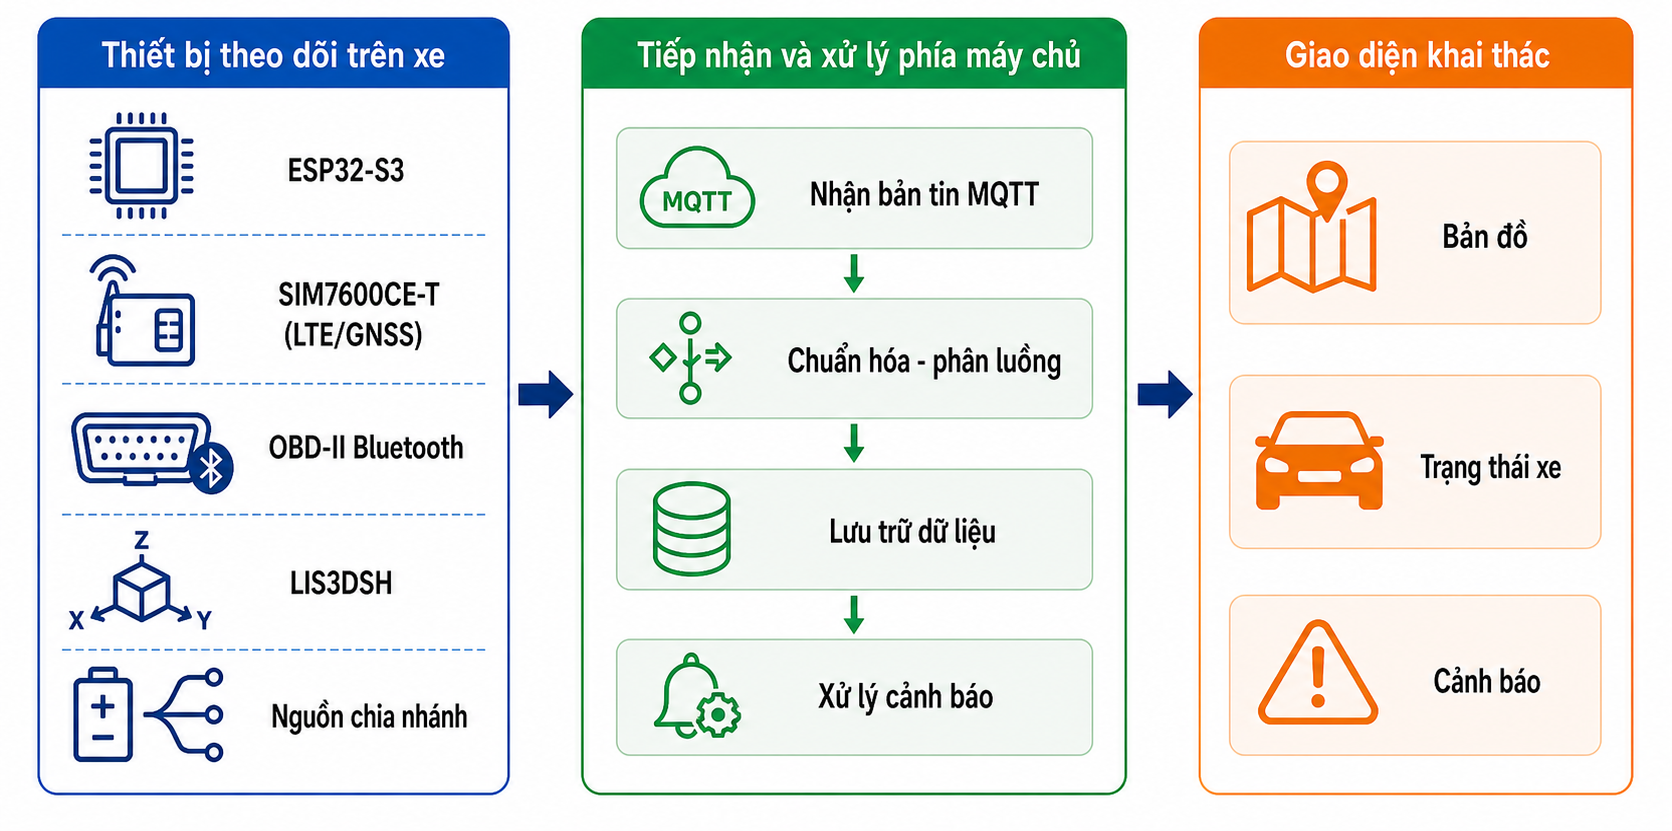
\includegraphics[keepaspectratio]{./assets/result/chapter-3-ai-figures/hinh-3-6-phuong-an-tong-the-duoc-chon-v2.png}}
\caption*{Hình 3.6: Phương án tổng thể của hệ thống được chọn}
\end{figure}

\emph{Hình 3.6: Kiến trúc tổng thể của phương án hệ thống được chọn}

Kiến trúc này làm rõ vai trò của từng khối trong toàn tuyến: thiết bị trên xe tạo bản tin giám sát,
máy chủ tiếp nhận và xử lý dữ liệu, còn giao diện giữ vai trò biểu diễn thông tin phục vụ khai thác.

\subsubsection{3.3.2. Phân tích chức năng các khối trong phương án được chọn}\label{phuxe2n-tuxedch-chux1ee9c-nux103ng-cuxe1c-khux1ed1i-trong-phux1b0ux1a1ng-uxe1n-ux111ux1b0ux1ee3c-chux1ecdn}

\begin{itemize}
\item
  \textbf{Khối 1 - Thiết bị theo dõi trên xe}

  \begin{itemize}
  \tightlist
  \item
    Vai trò của khối này là thu nhận trạng thái thực của phương tiện và tạo bản tin giám sát gửi về
    máy chủ.
  \item
    Ở khối này, ESP32-S3 giữ vai trò điều phối trung tâm; SIM7600CE-T đảm nhiệm truyền dữ liệu và
    định vị; \texttt{vgate\ iCar\ Pro} cung cấp dữ liệu OBD-II; LIS3DSH giữ nhánh phát hiện chuyển động khi
    xe đỗ; còn cấu trúc nguồn chia nhánh hỗ trợ chuyển giữa hoạt động và ngủ sâu.
  \item
    Với cách ghép đó, khối thiết bị đáp ứng đồng thời yêu cầu gọn, ít xâm lấn, đủ dữ liệu và có khả
    năng giảm tiêu thụ điện khi xe dừng lâu.
  \end{itemize}
\item
  \textbf{Khối 2 - Cụm tiếp nhận và xử lý dữ liệu ở máy chủ}

  \begin{itemize}
  \tightlist
  \item
    Vai trò của khối này là tiếp nhận bản tin từ thiết bị, chuẩn hóa, lưu trữ và xử lý dữ liệu trước
    khi cấp lại cho giao diện khai thác.
  \item
    Hướng tổ chức được chọn là tách lớp nhận bản tin khỏi lớp xử lý nghiệp vụ, đồng thời phân dữ liệu
    theo vai trò sử dụng.
  \item
    Cách tổ chức này cho phép hệ thống tiếp nhận tốt hơn các bản tin gửi dồn sau mất sóng, đồng thời
    giữ rõ phần tiếp nhận, phần xử lý và phần khai thác dữ liệu.
  \end{itemize}
\item
  \textbf{Khối 3 - Giao diện khai thác}

  \begin{itemize}
  \tightlist
  \item
    Vai trò của khối này là biểu diễn thông tin phục vụ theo dõi và cảnh báo trong quá trình vận hành.
  \item
    Giao diện được giữ theo hướng giao diện giám sát tập trung trên nền web, ưu tiên bản đồ, trạng thái xe và cảnh báo, còn
    dữ liệu kỹ thuật sâu hơn được đưa về các vùng tra cứu phụ.
  \item
    Nhờ đó, người sử dụng có thể theo dõi được các tín hiệu chính mà không bị dồn quá nhiều chi tiết
    kỹ thuật lên cùng một màn hình.
  \end{itemize}
\end{itemize}

Mối liên hệ giữa bốn nhóm ràng buộc kỹ thuật và các lựa chọn chính trong phương án được khái quát
trong Hình 3.7.

\begin{figure}[H]
\centering
\pandocbounded{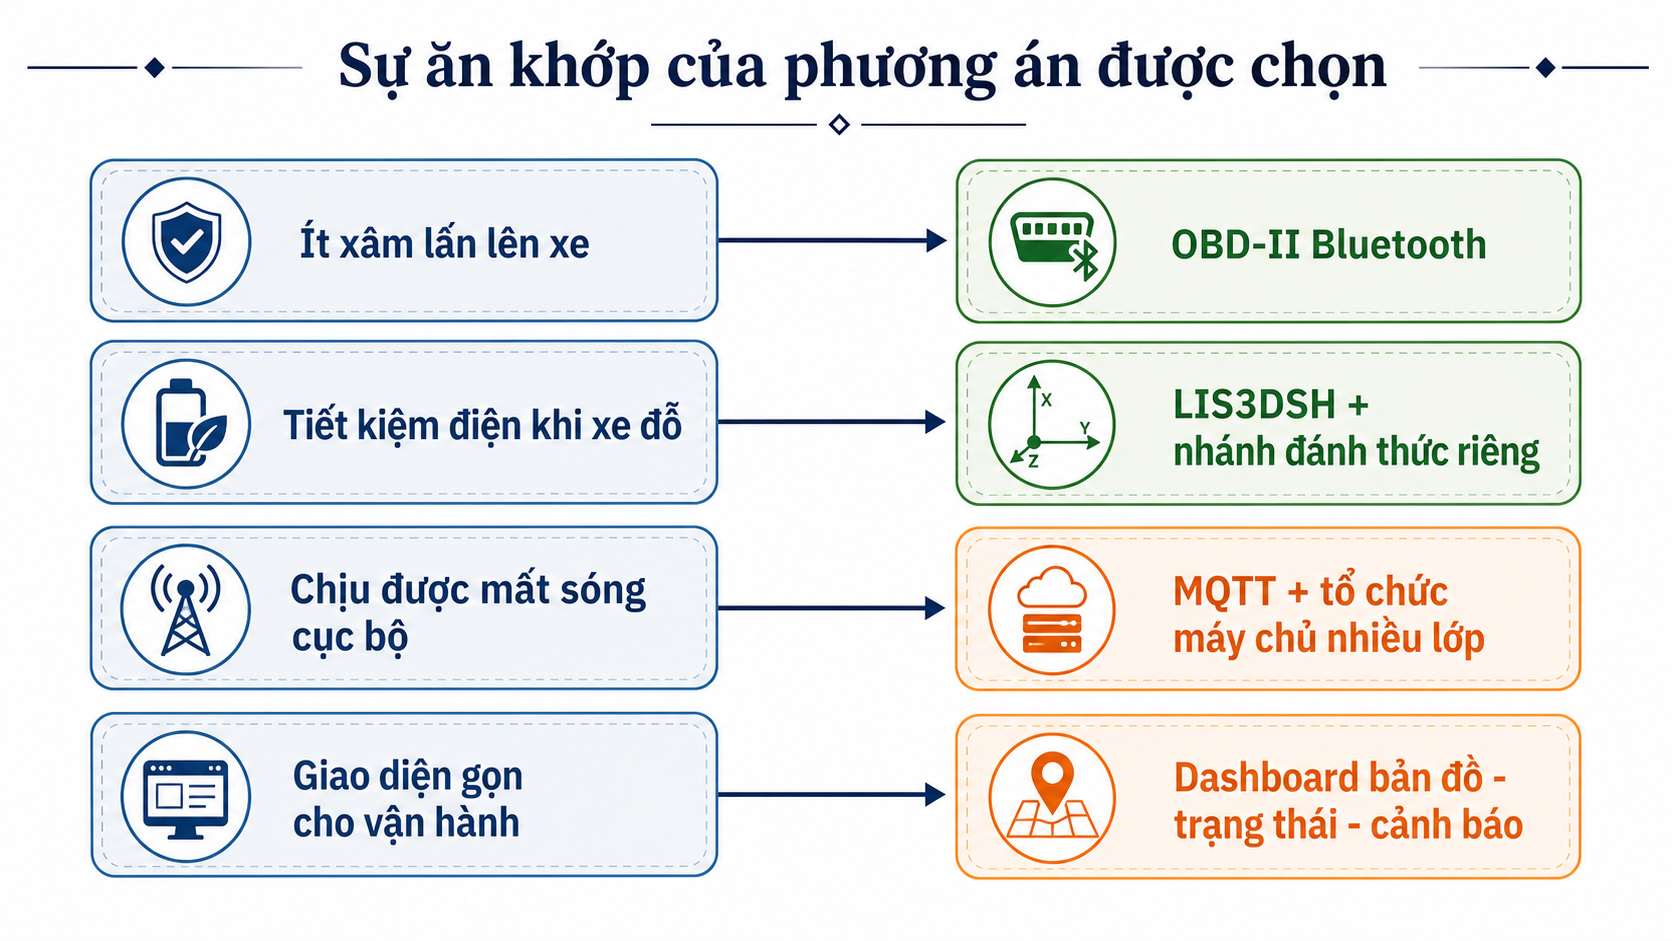
\includegraphics[keepaspectratio]{./assets/result/chapter-3-ai-figures/hinh-3-7-su-an-khop-cua-phuong-an-duoc-chon.png}}
\caption*{Hình 3.7: Sự ăn khớp của phương án được chọn}
\end{figure}

\emph{Hình 3.7: Mối liên hệ giữa các ràng buộc kỹ thuật và các lựa chọn chính của phương án}

\begin{itemize}
\item
  \textbf{Với yêu cầu ít xâm lấn lên xe}

  \begin{itemize}
  \tightlist
  \item
    Bộ đọc OBD-II Bluetooth giúp giảm dây tín hiệu phát sinh trong cabin và thuận tiện hơn khi chuyển
    lắp giữa nhiều xe.
  \item
    Mô-đun SIM7600CE-T tích hợp LTE và GNSS trong cùng một khối, từ đó giảm số phần cứng phải bố trí
    và điều khiển trên thiết bị.
  \end{itemize}
\item
  \textbf{Với yêu cầu tiết kiệm điện khi xe đỗ}

  \begin{itemize}
  \tightlist
  \item
    LIS3DSH kết hợp nhánh đánh thức riêng cho phép giữ lại đường phát hiện chuyển động với mức tiêu
    thụ thấp, trong khi các tải lớn có thể được đưa về ngủ sâu.
  \item
    Hướng phần mềm nhúng ESP-IDF kết hợp FreeRTOS tạo điều kiện thuận lợi hơn cho việc điều phối các
    nhánh tác vụ và tổ chức lại hoạt động của thiết bị theo từng trạng thái vận hành.
  \end{itemize}
\item
  \textbf{Với yêu cầu giữ ổn định tuyến truyền dữ liệu}

  \begin{itemize}
  \tightlist
  \item
    MQTT qua TLS phù hợp với bản tin nhỏ, phát sinh lặp lại và có thể bị gián đoạn bởi chất lượng
    mạng di động.
  \item
    Có bộ nhớ đệm cục bộ để lưu trữ dữ liệu trong trường hợp mất kết nối mạng hoàn toàn.
  \item
    Hướng tổ chức máy chủ theo broker, lớp trung gian và lưu trữ tách vai trò giúp tuyến dữ liệu chịu
    đựng tốt hơn khi thiết bị phải gửi bù dữ liệu sau mất sóng.
  \end{itemize}
\item
  \textbf{Với yêu cầu giao diện gọn cho vận hành}

  \begin{itemize}
  \tightlist
  \item
    Giao diện được giữ theo hướng giao diện giám sát tập trung trên nền web, ưu tiên bản đồ, trạng thái và cảnh báo.
  \item
    Cách tổ chức này giúp người vận hành theo dõi được thông tin chính mà không phải xử lý cùng lúc
    toàn bộ dữ liệu kỹ thuật phát sinh từ hệ thống.
  \end{itemize}
\end{itemize}

Nhìn chung, ba khối trong kiến trúc đã chọn giữ được cùng một mạch từ thiết bị, máy chủ đến giao
diện khai thác, nên có thể xem là phương án khả thi cho bài toán của đồ án.

\subsection{3.4. Tối ưu phương án thiết kế}\label{tux1ed1i-ux1b0u-phux1b0ux1a1ng-uxe1n-thiux1ebft-kux1ebf}

Từ phần phân tích ở Mục 3.1, phần đề xuất và so sánh ở Mục 3.2, cùng phương án khả thi ở Mục 3.3,
cấu hình thiết kế tổng thể của hệ thống theo dõi xe được tổng hợp trong Bảng 3.8.

\textbf{Bảng 3.8: Bảng tổng hợp cấu hình hệ thống theo dõi xe}

{\def\LTcaptype{none} % do not increment counter
\begin{longtable}[]{@{}
  >{\raggedright\arraybackslash}p{(\linewidth - 6\tabcolsep) * \real{0.1033}}
  >{\raggedright\arraybackslash}p{(\linewidth - 6\tabcolsep) * \real{0.1549}}
  >{\raggedright\arraybackslash}p{(\linewidth - 6\tabcolsep) * \real{0.2958}}
  >{\raggedright\arraybackslash}p{(\linewidth - 6\tabcolsep) * \real{0.4460}}@{}}
\toprule\noalign{}
\begin{minipage}[b]{\linewidth}\raggedright
Phân hệ
\end{minipage} & \begin{minipage}[b]{\linewidth}\raggedright
Hạng mục
\end{minipage} & \begin{minipage}[b]{\linewidth}\raggedright
Phương án / thông số đã chọn
\end{minipage} & \begin{minipage}[b]{\linewidth}\raggedright
Ghi chú kỹ thuật
\end{minipage} \\
\midrule\noalign{}
\endhead
\bottomrule\noalign{}
\endlastfoot
1. Thiết bị trên xe & Bộ điều khiển trung tâm & ESP32-S3 & Điều phối modem LTE/GNSS, BLE OBD-II, IMU và các nhánh nguồn \\
1. Thiết bị trên xe & Truyền dữ liệu và định vị & SIM7600CE-T & Tích hợp LTE và GNSS trong cùng một mô-đun \\
1. Thiết bị trên xe & Thu dữ liệu vận hành & \texttt{vgate\ iCar\ Pro} qua Bluetooth & Lấy nhóm dữ liệu quản lý qua OBD-II, giảm dây nối trong cabin \\
1. Thiết bị trên xe & Giám sát khi xe đỗ & LIS3DSH + nhánh đánh thức riêng & Giữ phát hiện chuyển động khi phần tải lớn đã đưa về ngủ sâu \\
1. Thiết bị trên xe & Nguồn cấp & Nguồn chia nhánh + pin dự phòng + bảo vệ điện áp thấp & Tách nhánh luôn cấp và nhánh tải lớn, hạn chế ảnh hưởng lên ắc quy xe \\
1. Thiết bị trên xe & Nền tảng firmware & ESP-IDF + FreeRTOS & Phù hợp khi thiết bị phải điều phối nhiều ngoại vi và nhiều trạng thái \\
2. Máy chủ & Giao thức truyền bản tin & MQTT qua TLS & Phù hợp với bản tin nhỏ, lặp lại và có thể gián đoạn theo mạng di động \\
2. Máy chủ & Tiếp nhận và xử lý dữ liệu & Broker + lớp trung gian + lưu trữ tách vai trò & Tách lớp nhận bản tin, xử lý và lưu trữ để thuận lợi hơn khi mở rộng \\
3. Khai thác & Giao diện quản lý & Giao diện giám sát tập trung trên nền web & Ưu tiên thông tin phục vụ vận hành; dữ liệu sâu hơn được đưa về vùng tra cứu \\
\end{longtable}
}

\section{CHƯƠNG 4. TRIỂN KHAI GIẢI PHÁP VÀ KẾT QUẢ - IMPLEMENTATION AND RESULTS}\label{chux1b0ux1a1ng-4.-triux1ec3n-khai-giux1ea3i-phuxe1p-vuxe0-kux1ebft-quux1ea3---implementation-and-results}


\chapterheading{CHƯƠNG 4. TRIỂN KHAI GIẢI PHÁP VÀ KẾT QUẢ -- IMPLEMENTATION AND RESULTS}

Chương 4 trình bày kết quả hiện thực các phương án đã lựa chọn ở Chương 3 thành
hệ thống hoàn chỉnh. Khác với Chương 3 tập trung vào cơ sở lựa chọn giải pháp,
chương này tập trung vào các hạng mục đã được triển khai thực tế, mức độ hoàn
thành của từng lớp và kết quả tích hợp toàn tuyến. Trong phạm vi đồ án, các hạng
mục cốt lõi gồm phần cứng thiết bị theo dõi, firmware nhúng, hạ tầng máy chủ đám
mây, dịch vụ backend, giao diện frontend và lớp quan sát vận hành đều đã được
hoàn thành và đưa vào sử dụng.

\subsection{4.1. Triển khai phần cứng thiết bị - Hardware implementation}\label{triux1ec3n-khai-phux1ea7n-cux1ee9ng-thiux1ebft-bux1ecb---hardware-implementation}

\subsubsection{4.1.1. Hoàn thiện hồ sơ thiết kế và bảng mạch in}\label{houxe0n-thiux1ec7n-hux1ed3-sux1a1-thiux1ebft-kux1ebf-vuxe0-bux1ea3ng-mux1ea1ch-in}

Phần cứng thiết bị đã được triển khai theo hướng bo mạch chuyên dụng thay cho mô
hình ghép nhiều bo phát triển rời. Hồ sơ thiết kế đã được hoàn thiện cho toàn bộ
các khối chính gồm xử lý trung tâm ESP32-S3, modem 4G/GNSS SIM7600CE-T, cảm biến
gia tốc LIS3DH, đồng hồ thời gian thực DS3231M, thẻ nhớ microSD, mạch đo điện áp,
khối nguồn logic, khối nguồn modem và khối nguồn dự phòng. Việc hoàn thiện đồng
thời sơ đồ nguyên lý, bố trí PCB và ánh xạ chân đã tạo ra một nền tảng nhất quán
giữa thiết kế mạch và firmware.

{\thesissetfigureid{4.1}{condensed-hinh-4-1-so-do-dau-noi-tong-the-giua-esp32-s3-va-cac-khoi-phan-cung-tich-hop}
\begin{figure}[H]
\centering
\pandocbounded{\safeincludesvg{./assets/figures/07-chuong-4-trien-khai-hardware-hinh-4-5.svg}}
\caption{Sơ đồ đấu nối tổng thể giữa ESP32-S3 và các khối phần cứng tích hợp}
\label{fig:condensed-hinh-4-1-so-do-dau-noi-tong-the-giua-esp32-s3-va-cac-khoi-phan-cung-tich-hop}
\end{figure}
}

\emph{\textbf{TODO/BLOCKER:} Chưa xuất ảnh kiểm chứng đúng tỷ lệ cho các hình phụ Hình 4.1a-4.1d gồm sơ đồ nguyên lý tổng thể, sơ đồ nguyên lý chi tiết và bố trí PCB mặt trên/mặt dưới. Không đánh số hình và không đưa vào danh mục hình cho đến khi có asset xuất trực tiếp từ hồ sơ thiết kế phần cứng.}

{\thesissettableid{4.1}{condensed-bang-4-1-cac-hang-muc-thiet-ke-phan-cung-da-hoan-thanh}
\def\LTcaptype{table}
\begin{longtable}{|L{0.166\linewidth}|L{0.419\linewidth}|L{0.373\linewidth}|}
\caption{Các hạng mục thiết kế phần cứng đã hoàn thành}\label{tab:condensed-bang-4-1-cac-hang-muc-thiet-ke-phan-cung-da-hoan-thanh}\\
\hline
\textbf{Hạng mục thiết kế} & \textbf{Kết quả triển khai} & \textbf{Ý nghĩa đối với chỉ tiêu phần cứng} \\
\hline
\endfirsthead
\caption[]{Các hạng mục thiết kế phần cứng đã hoàn thành (tiếp theo)}\\
\hline
\textbf{Hạng mục thiết kế} & \textbf{Kết quả triển khai} & \textbf{Ý nghĩa đối với chỉ tiêu phần cứng} \\
\hline
\endhead
\endfoot
\endlastfoot
Sơ đồ nguyên lý theo khối & Đã hoàn thiện sơ đồ cho khối xử lý, modem, nguồn, cảm biến và lưu trữ cục bộ & Bảo đảm thiết bị có thể tích hợp đầy đủ chức năng trên cùng một bo mạch \\\hline
Bảng mạch in PCB & Đã hoàn thiện bố trí PCB chuyên dụng phục vụ gia công nguyên mẫu & Đáp ứng yêu cầu nhỏ gọn để lắp đặt trên xe thật \\\hline
Ánh xạ chân phần cứng - firmware & Đã chốt các chân UART, I2C, ADC, SDMMC, ngắt cảm biến và điều khiển nguồn & Giảm sai lệch giữa thiết kế mạch và mã nguồn nhúng \\\hline
Kiến trúc nguồn chính và dự phòng & Đã tích hợp nhánh nguồn logic, nhánh nguồn modem và nguồn dự phòng trên cùng thiết kế & Hỗ trợ mục tiêu vận hành ổn định khi điện áp xe dao động \\\hline
Hồ sơ phục vụ chế tạo & Đã xuất bộ tệp phục vụ gia công, lắp ráp và kiểm tra nguyên mẫu & Cho phép chuyển từ giai đoạn thiết kế sang nguyên mẫu thật \\\hline
\end{longtable}
}

\emph{\textbf{TODO/BLOCKER:} Chưa đưa Bảng 4.1A/4.1B vào bản condensed vì BOM chi tiết và bảng tổng hợp chi phí linh kiện cần được đối chiếu lại với hồ sơ thiết kế cuối. Không đánh số bảng và không đưa vào danh mục bảng cho đến khi có dữ liệu BOM đã chốt.}

\subsubsection{4.1.2. Gia công, lắp ráp và tích hợp nguyên mẫu}\label{gia-cuxf4ng-lux1eafp-ruxe1p-vuxe0-tuxedch-hux1ee3p-nguyuxean-mux1eabu}

Sau khi chốt thiết kế, bo mạch PCB đã được gia công và hàn lắp đầy đủ linh kiện
chính. Nguyên mẫu phần cứng vì vậy không còn dừng ở mức hồ sơ thiết kế, mà đã
được hiện thực thành thiết bị thật để nạp firmware, kiểm tra tương tác giữa các
ngoại vi và đánh giá khả năng lắp đặt trên xe. Trên nguyên mẫu này, các kết nối
quan trọng đã được đưa vào vận hành đúng theo cấu hình thiết kế: modem dùng UART
riêng; LIS3DH và DS3231M dùng chung bus I2C; hai kênh ADC theo dõi nguồn xe và
nguồn dự phòng; microSD phục vụ lưu đệm cục bộ; bộ chuyển đổi OBD2 BLE giao tiếp
không dây với thiết bị.

{\thesissettableid{4.2}{condensed-bang-4-2-ket-qua-tich-hop-phan-cung-tren-nguyen-mau-that}
\def\LTcaptype{table}
\begin{longtable}{|L{0.254\linewidth}|L{0.588\linewidth}|L{0.116\linewidth}|}
\caption{Kết quả tích hợp phần cứng trên nguyên mẫu thật}\label{tab:condensed-bang-4-2-ket-qua-tich-hop-phan-cung-tren-nguyen-mau-that}\\
\hline
\textbf{Hạng mục tích hợp} & \textbf{Kết quả đạt được} & \textbf{Mức độ hoàn thành} \\
\hline
\endfirsthead
\caption[]{Kết quả tích hợp phần cứng trên nguyên mẫu thật (tiếp theo)}\\
\hline
\textbf{Hạng mục tích hợp} & \textbf{Kết quả đạt được} & \textbf{Mức độ hoàn thành} \\
\hline
\endhead
\endfoot
\endlastfoot
Khối nguồn và bảo vệ & Các nhánh nguồn chính, nguồn logic và nguồn dự phòng đã được lắp ráp đầy đủ & Hoàn thành \\\hline
Khối modem 4G/GNSS & Đã tích hợp modem SIM7600CE-T cho kết nối dữ liệu và định vị & Hoàn thành \\\hline
Khối cảm biến và đồng hồ thời gian thực & LIS3DH và DS3231M đã được ghép lên bo mạch và chạy cùng firmware & Hoàn thành \\\hline
Khối đo điện áp & Hai kênh ADC đã được hiện thực để giám sát nguồn xe và pin dự phòng & Hoàn thành \\\hline
Khối lưu trữ cục bộ & microSD đã được tích hợp để lưu đệm khi mất mạng & Hoàn thành \\\hline
Cấu hình lắp đặt trên xe & Thiết bị đã được ghép với nguồn trên xe và bộ chuyển đổi OBD2 BLE trong cấu hình thử nghiệm & Hoàn thành \\\hline
\end{longtable}
}

\emph{\textbf{TODO/BLOCKER:} Chưa có ảnh thật đã kiểm chứng cho Hình 4.2 - ảnh PCB sau khi gia công và hàn lắp đầy đủ linh kiện. Không đánh số hình và không đưa vào danh mục hình cho đến khi có asset đúng nội dung.}

\emph{\textbf{TODO/BLOCKER:} Chưa có ảnh thật đã kiểm chứng cho Hình 4.3 - ảnh thiết bị sau khi lắp đặt trên xe thử nghiệm. Không đánh số hình và không đưa vào danh mục hình cho đến khi có asset đúng nội dung.}

\subsection{4.2. Triển khai firmware thiết bị - Firmware implementation}\label{triux1ec3n-khai-firmware-thiux1ebft-bux1ecb---firmware-implementation}

\subsubsection{4.2.1. Tổ chức mã nguồn firmware}\label{tux1ed5-chux1ee9c-muxe3-nguux1ed3n-firmware}

Firmware được phát triển trên nền ESP-IDF và FreeRTOS theo cấu trúc phân lớp đã
đề xuất ở Chương 3. Cách tổ chức này không chỉ phục vụ việc lập trình từng ngoại
vi riêng lẻ, mà hướng tới một firmware có khả năng vận hành lâu dài trên thiết bị
thật, trong đó ranh giới giữa lớp phần cứng, lớp thích nghi ngoại vi, lớp chức
năng nghiệp vụ và lớp điều phối được giữ rõ ràng.

{\thesissettableid{4.3}{condensed-bang-4-3-cac-nhom-mo-dun-chinh-da-duoc-hien-thuc-trong-firmware}
\def\LTcaptype{table}
\begin{longtable}{|L{0.115\linewidth}|L{0.523\linewidth}|L{0.321\linewidth}|}
\caption{Các nhóm mô-đun chính đã được hiện thực trong firmware}\label{tab:condensed-bang-4-3-cac-nhom-mo-dun-chinh-da-duoc-hien-thuc-trong-firmware}\\
\hline
\textbf{Nhóm mô-đun} & \textbf{Thành phần tiêu biểu} & \textbf{Vai trò trong hệ thống} \\
\hline
\endfirsthead
\caption[]{Các nhóm mô-đun chính đã được hiện thực trong firmware (tiếp theo)}\\
\hline
\textbf{Nhóm mô-đun} & \textbf{Thành phần tiêu biểu} & \textbf{Vai trò trong hệ thống} \\
\hline
\endhead
\endfoot
\endlastfoot
Nền tảng phần cứng & \thesisterm{platform-board-esp32s3}, \thesisterm{platform-hal-esp-idf} & Khởi tạo bo mạch, GPIO, ADC, UART, I2C, SPI, SDMMC và các dịch vụ nền \\\hline
Bộ thích nghi ngoại vi & \thesisterm{adapter-modem-sim7600-at}, \thesisterm{adapter-mqtt-sim7600-at}, \thesisterm{adapter-ble-obd-nimble}, \thesisterm{adapter-rtc-ds3231m}, \thesisterm{adapter-storage-sdmmc-fatfs}, \thesisterm{adapter-kv-nvs} & Điều khiển modem, MQTT, BLE OBD2, đồng hồ thời gian thực, microSD và bộ nhớ cấu hình \\\hline
Miền chức năng & \thesisterm{domain-connectivity}, \thesisterm{domain-telemetry}, \thesisterm{domain-obd}, \thesisterm{domain-storage}, \thesisterm{domain-ota} & Xử lý kết nối, dữ liệu đo từ xa telemetry, dữ liệu OBD, lưu đệm và cập nhật firmware \\\hline
Điều phối ứng dụng & \thesisterm{app-core} & Khởi động hệ thống, điều phối máy trạng thái và vòng vận hành chính \\\hline
Dữ liệu và tiện ích dùng chung & \thesisterm{contracts-device-cloud}, \thesisterm{shared-kernel} & Chuẩn hóa cấu trúc dữ liệu thiết bị - máy chủ và các kiểu dữ liệu dùng chung \\\hline
\end{longtable}
}

\subsubsection{4.2.2. Hiện thực các chức năng cốt lõi trên thiết bị}\label{hiux1ec7n-thux1ef1c-cuxe1c-chux1ee9c-nux103ng-cux1ed1t-luxf5i-truxean-thiux1ebft-bux1ecb}

Trên phần cứng thật, firmware đã được hiện thực đầy đủ cho các nhóm chức năng cốt
lõi của thiết bị theo dõi. Sau khi cấp nguồn hoặc được đánh thức, hệ thống nạp
cấu hình, xác định nguyên nhân đánh thức, đưa toàn bộ ngoại vi vào trạng thái phù
hợp và điều phối vòng vận hành trung tâm. Dữ liệu đo từ xa (telemetry) và dữ liệu
OBD được đóng gói thành các bản tin MQTT thống nhất với phía cloud; các bản ghi
chưa gửi được sẽ được lưu đệm trên microSD; luồng OTA cũng đã được tích hợp để
hỗ trợ cập nhật firmware từ xa.

{\thesissetfigureid{4.4}{condensed-hinh-4-4-luu-do-thuat-toan-chinh-cua-firmware-thiet-bi-theo-doi}
\begin{figure}[H]
\centering
\pandocbounded{\safeincludesvg{./assets/figures/08-chuong-4-trien-khai-firmware-hinh-4-17.svg}}
\caption{Lưu đồ thuật toán chính của firmware thiết bị theo dõi}
\label{fig:condensed-hinh-4-4-luu-do-thuat-toan-chinh-cua-firmware-thiet-bi-theo-doi}
\end{figure}
}

{\thesissettableid{4.4}{condensed-bang-4-4-cac-nhom-chuc-nang-firmware-da-duoc-hien-thuc}
\def\LTcaptype{table}
\begin{longtable}{|L{0.168\linewidth}|L{0.508\linewidth}|L{0.282\linewidth}|}
\caption{Các nhóm chức năng firmware đã được hiện thực}\label{tab:condensed-bang-4-4-cac-nhom-chuc-nang-firmware-da-duoc-hien-thuc}\\
\hline
\textbf{Nhóm chức năng cốt lõi} & \textbf{Kết quả triển khai} & \textbf{Liên hệ với chỉ tiêu firmware} \\
\hline
\endfirsthead
\caption[]{Các nhóm chức năng firmware đã được hiện thực (tiếp theo)}\\
\hline
\textbf{Nhóm chức năng cốt lõi} & \textbf{Kết quả triển khai} & \textbf{Liên hệ với chỉ tiêu firmware} \\
\hline
\endhead
\endfoot
\endlastfoot
Khởi động và điều phối trạng thái & Nạp cấu hình, nhận biết nguyên nhân đánh thức, điều phối trạng thái thiết bị, trạng thái di chuyển và trạng thái OBD & Đáp ứng yêu cầu quản lý nhiều trạng thái vận hành \\\hline
Kết nối modem, GNSS và MQTT & Điều khiển SIM7600CE-T, thiết lập 4G, lấy dữ liệu GNSS và truyền bản tin MQTT theo cây topic đã chuẩn hóa & Đáp ứng yêu cầu thu thập, đóng gói và gửi dữ liệu cần thiết \\\hline
Đọc OBD2 qua BLE & Duy trì kết nối với bộ chuyển đổi OBD2 BLE, đọc PID và nhóm DTC chẩn đoán cơ bản & Đáp ứng yêu cầu khai thác dữ liệu vận hành từ xe mà ít xâm lấn \\\hline
Giám sát nguồn và trạng thái đánh lửa & Đo nguồn xe, nguồn dự phòng, suy luận trạng thái đánh lửa và điều chỉnh hành vi thiết bị theo trạng thái xe & Đáp ứng yêu cầu phản ứng theo bối cảnh vận hành \\\hline
Lưu đệm ngoại tuyến & Ghi bản tin lên microSD và phát lại theo thứ tự khi kết nối phục hồi & Đáp ứng yêu cầu hạn chế mất dữ liệu khi mạng gián đoạn \\\hline
Cập nhật firmware từ xa & Hỗ trợ luồng OTA, tiếp nhận lệnh, báo tiến trình và phản hồi kết quả cập nhật & Tăng khả năng bảo trì thiết bị sau khi đã lắp trên xe \\\hline
\end{longtable}
}

\subsubsection{4.2.3. Các PID và nhóm mã lỗi DTC OBD đã hiện thực}\label{cuxe1c-pid-vuxe0-nhuxf3m-muxe3-lux1ed7i-dtc-obd-ux111uxe3-hiux1ec7n-thux1ef1c}

Phần OBD trong firmware được tổ chức theo hướng ưu tiên các tham số chẩn đoán cơ
bản, có giá trị trực tiếp cho bài toán giám sát phương tiện và vẫn phù hợp với bộ
chuyển đổi OBD2 BLE. Tại thời điểm hoàn thiện đồ án, firmware đã đọc được các PID
và các nhóm mã lỗi DTC nêu trong các bảng sau.

{\thesissettableid{4.5}{condensed-bang-4-5-cac-pid-obd-ii-dang-duoc-firmware-thu-nhan}
\def\LTcaptype{table}
\begin{longtable}{|L{0.095\linewidth}|L{0.190\linewidth}|L{0.350\linewidth}|L{0.315\linewidth}|}
\caption{Các PID OBD-II đang được firmware thu nhận}\label{tab:condensed-bang-4-5-cac-pid-obd-ii-dang-duoc-firmware-thu-nhan}\\
\hline
\textbf{Chế độ/}\newline\textbf{PID} & \textbf{Thông số} & \textbf{Ý nghĩa sử dụng trong hệ thống} & \textbf{Cách biểu diễn trong dữ liệu} \\
\hline
\endfirsthead
\caption[]{Các PID OBD-II đang được firmware thu nhận (tiếp theo)}\\
\hline
\textbf{Chế độ/}\newline\textbf{PID} & \textbf{Thông số} & \textbf{Ý nghĩa sử dụng trong hệ thống} & \textbf{Cách biểu diễn trong dữ liệu} \\
\hline
\endhead
\endfoot
\endlastfoot
\thesisterm{01\ 01} & Trạng thái giám sát, đèn MIL và số lượng DTC & Xác định xe đang có cờ lỗi động cơ hay không, đồng thời lấy ảnh chụp trạng thái readiness & \thesisterm{mil\_on}, \thesisterm{reported\_dtc\_count}, \thesisterm{readiness.*} \\\hline
\thesisterm{01\ 0C} & Vòng tua động cơ & Hỗ trợ suy luận trạng thái đánh lửa và trạng thái vận hành thực của xe & \thesisterm{diagnostics.signals.}\newline\thesisterm{rpm} \\\hline
\thesisterm{01\ 0D} & Tốc độ xe theo ECU & Đối chiếu với tốc độ GNSS và bổ sung dữ liệu vận hành & \thesisterm{diagnostics.signals.}\newline\thesisterm{obd\_speed\_kph} \\\hline
\thesisterm{01\ 05} & Nhiệt độ nước làm mát & Phản ánh trạng thái nhiệt của động cơ trong khi vận hành & \thesisterm{diagnostics.signals.}\newline\thesisterm{coolant\_c} \\\hline
\thesisterm{01\ 2F} & Mức nhiên liệu & Cung cấp thông tin phục vụ theo dõi nhiên liệu ở mức cơ bản & \thesisterm{diagnostics.signals.}\newline\thesisterm{fuel\_level\_pct} \\\hline
\thesisterm{01\ 04} & Tải động cơ & Bổ sung góc nhìn về mức tải tức thời của động cơ & \thesisterm{diagnostics.signals.}\newline\thesisterm{engine\_load\_pct} \\\hline
\end{longtable}
}

{\thesissettableid{4.6}{condensed-bang-4-6-cac-nhom-ma-loi-dtc-dang-duoc-firmware-thu-nhan}
\def\LTcaptype{table}
\begin{longtable}{|L{0.083\linewidth}|L{0.065\linewidth}|L{0.396\linewidth}|L{0.074\linewidth}|L{0.326\linewidth}|}
\caption{Các nhóm mã lỗi DTC đang được firmware thu nhận}\label{tab:condensed-bang-4-6-cac-nhom-ma-loi-dtc-dang-duoc-firmware-thu-nhan}\\
\hline
\textbf{Nhóm DTC} & \textbf{Chế độ đọc} & \textbf{Ý nghĩa} & \textbf{Ví dụ minh họa} & \textbf{Cách trình bày trên hệ thống} \\
\hline
\endfirsthead
\caption[]{Các nhóm mã lỗi DTC đang được firmware thu nhận (tiếp theo)}\\
\hline
\textbf{Nhóm DTC} & \textbf{Chế độ đọc} & \textbf{Ý nghĩa} & \textbf{Ví dụ minh họa} & \textbf{Cách trình bày trên hệ thống} \\
\hline
\endhead
\endfoot
\endlastfoot
DTC đang lưu & \thesisterm{03} & Các mã lỗi hiện đang được ECU lưu giữ, phản ánh lỗi đã được xác nhận & \thesisterm{P0500} & Mảng \thesisterm{dtc.stored} trong payload MQTT và giao diện chi tiết thiết bị \\\hline
DTC chờ xác nhận & \thesisterm{07} & Các mã lỗi mới xuất hiện, chưa đủ điều kiện để xác nhận là lỗi ổn định & \thesisterm{P0171} & Mảng \thesisterm{dtc.pending} để hỗ trợ theo dõi xu hướng phát sinh lỗi \\\hline
DTC thường trực & \thesisterm{0A} & Các mã lỗi vẫn còn bị ECU ghi nhận sau nhiều chu kỳ vận hành & \thesisterm{P0171} & Mảng \thesisterm{dtc.permanent} để phục vụ bảo trì và chẩn đoán sâu hơn \\\hline
\end{longtable}
}

Các mã DTC được biểu diễn theo định dạng năm ký tự chuẩn như \thesisterm{P0171}, trong đó ký
tự đầu cho biết nhóm hệ thống lỗi. Cách tổ chức này cho phép frontend hiển thị rõ
từng nhóm lỗi, đồng thời vẫn giữ nguyên tính tương thích với dữ liệu gốc do ECU trả
về.

\subsection{4.3. Triển khai hệ thống cloud - Cloud implementation}\label{triux1ec3n-khai-hux1ec7-thux1ed1ng-cloud---cloud-implementation}

\subsubsection{4.3.1. Hạ tầng triển khai trên cloud VPS}\label{hux1ea1-tux1ea7ng-triux1ec3n-khai-truxean-cloud-vps}

Hệ thống phía máy chủ đã được triển khai trên cloud VPS thay cho mô hình chỉ chạy
cục bộ. Kiến trúc triển khai sử dụng Docker Compose theo từng dịch vụ, trong đó
mỗi thành phần có Dockerfile và tệp cấu hình riêng, đồng thời cùng tham gia mạng
chia sẻ \thesisterm{tracking-network}. Mô hình này phù hợp với hướng kiến trúc nhiều dịch vụ
đã lựa chọn ở Chương 3, giúp tách rõ tuyến tiếp nhận dữ liệu thiết bị, lớp lưu
trữ, lớp xử lý nghiệp vụ và lớp giao diện quản trị.

{\thesissetfigureid{4.5}{condensed-hinh-4-5-kien-truc-tong-the-he-thong-may-chu-va-luong-du-lieu}
\begin{figure}[H]
\centering
\pandocbounded{\safeincludesvg{./assets/figures/09-chuong-4-trien-khai-cloud-hinh-4-15.svg}}
\caption{Kiến trúc tổng thể hệ thống máy chủ và luồng dữ liệu}
\label{fig:condensed-hinh-4-5-kien-truc-tong-the-he-thong-may-chu-va-luong-du-lieu}
\end{figure}
}

{\thesissettableid{4.7}{condensed-bang-4-7-cac-dich-vu-da-duoc-trien-khai-tren-cloud-vps}
\def\LTcaptype{table}
\begin{longtable}{|L{0.210\linewidth}|L{0.300\linewidth}|L{0.320\linewidth}|L{0.120\linewidth}|}
\caption{Các dịch vụ đã được triển khai trên cloud VPS}\label{tab:condensed-bang-4-7-cac-dich-vu-da-duoc-trien-khai-tren-cloud-vps}\\
\hline
\textbf{Dịch vụ} & \textbf{Vai trò chính} & \textbf{Kết quả triển khai} & \textbf{Trạng thái} \\
\hline
\endfirsthead
\caption[]{Các dịch vụ đã được triển khai trên cloud VPS (tiếp theo)}\\
\hline
\textbf{Dịch vụ} & \textbf{Vai trò chính} & \textbf{Kết quả triển khai} & \textbf{Trạng thái} \\
\hline
\endhead
\endfoot
\endlastfoot
PostgreSQL/\newline PostGIS & Lưu dữ liệu nghiệp vụ, dữ liệu quan hệ và dữ liệu không gian & Đã triển khai và khởi tạo đầy đủ lược đồ dữ liệu của hệ thống & Hoàn thành \\\hline
EMQX & Tiếp nhận kết nối MQTT từ thiết bị và phân phối bản tin & Đã triển khai làm broker trung tâm của hệ thống & Hoàn thành \\\hline
VictoriaMetrics & Lưu dữ liệu đo từ xa theo chuỗi thời gian & Đã triển khai làm kho dữ liệu chỉ số và lịch sử dữ liệu đo từ xa & Hoàn thành \\\hline
VictoriaLogs & Thu thập nhật ký tập trung từ các dịch vụ & Đã triển khai phục vụ truy vết sự cố và vận hành & Hoàn thành \\\hline
MQTT Bridge & Tiếp nhận bản tin từ EMQX, kiểm tra payload và phân luồng lưu trữ & Đã triển khai thành dịch vụ độc lập & Hoàn thành \\\hline
Backend & Xử lý nghiệp vụ và cung cấp REST API, WebSocket & Đã triển khai thành dịch vụ ứng dụng độc lập & Hoàn thành \\\hline
Frontend & Cung cấp giao diện quản trị web & Đã triển khai thành dịch vụ công khai qua tên miền riêng & Hoàn thành \\\hline
Grafana & Quan sát chỉ số và nhật ký vận hành & Đã triển khai phục vụ lớp quan sát hệ thống & Hoàn thành \\\hline
Nginx Proxy Manager & Công bố dịch vụ ra Internet, phân tách tên miền và luồng truy cập & Đã triển khai làm lớp chuyển tiếp ngược của hệ thống & Hoàn thành \\\hline
\end{longtable}
}

\subsubsection{4.3.2. MQTT broker, bản tin MQTT và các lớp lưu trữ}\label{mqtt-broker-bux1ea3n-tin-mqtt-vuxe0-cuxe1c-lux1edbp-lux1b0u-trux1eef}

Ở lớp tiếp nhận dữ liệu, EMQX giữ vai trò broker MQTT trung tâm. Thiết bị gửi dữ
liệu theo cây topic đã chuẩn hóa; MQTT Bridge đăng ký nhận bốn nhóm topic chính
gồm \thesisterm{rawdata}, \thesisterm{status}, \thesisterm{events} và \thesisterm{firmware}; backend phát lệnh điều khiển theo
topic \thesisterm{commands}. Cấu trúc này giúp tách rõ dữ liệu đo từ xa, trạng thái, sự kiện
và tiến trình cập nhật firmware.

{\thesissettableid{4.8}{condensed-bang-4-8-cay-topic-mqtt-dang-duoc-su-dung-trong-he-thong}
\def\LTcaptype{table}
\begin{longtable}{|L{0.190\linewidth}|L{0.125\linewidth}|L{0.055\linewidth}|L{0.330\linewidth}|L{0.250\linewidth}|}
\caption{Cây topic MQTT đang được sử dụng trong hệ thống}\label{tab:condensed-bang-4-8-cay-topic-mqtt-dang-duoc-su-dung-trong-he-thong}\\
\hline
\textbf{Topic} & \textbf{Hướng truyền} & \textbf{QoS} & \textbf{Nội dung chính} & \textbf{Ghi chú triển khai} \\
\hline
\endfirsthead
\caption[]{Cây topic MQTT đang được sử dụng trong hệ thống (tiếp theo)}\\
\hline
\textbf{Topic} & \textbf{Hướng truyền} & \textbf{QoS} & \textbf{Nội dung chính} & \textbf{Ghi chú triển khai} \\
\hline
\endhead
\endfoot
\endlastfoot
\thesisterm{v1/}\newline\thesisterm{\{device\_id\}/}\newline\thesisterm{rawdata} & Thiết bị -\textgreater{} máy chủ & \thesisterm{0} & Bản tin dữ liệu đo từ xa chính: GNSS, điện áp, trạng thái và mẫu OBD tức thời & Tần suất cao, ưu tiên giảm tải đường truyền \\\hline
\thesisterm{v1/}\newline\thesisterm{\{device\_id\}/}\newline\thesisterm{status} & Thiết bị -\textgreater{} máy chủ & \thesisterm{1} & Heartbeat, trạng thái phiên và trạng thái thiết bị & Hạn chế mất bản tin vì dùng cho theo dõi thiết bị online/offline \\\hline
\thesisterm{v1/}\newline\thesisterm{\{device\_id\}/}\newline\thesisterm{events} & Thiết bị -\textgreater{} máy chủ & \thesisterm{1} & Cảnh báo và sự kiện quan trọng & Phục vụ truy vết sự cố và cảnh báo vận hành \\\hline
\thesisterm{v1/}\newline\thesisterm{\{device\_id\}/}\newline\thesisterm{firmware} & Thiết bị -\textgreater{} máy chủ & \thesisterm{1} & Trạng thái OTA, tiến trình cập nhật và kết quả & Phục vụ truy vết luồng cập nhật firmware \\\hline
\thesisterm{v1/}\newline\thesisterm{\{device\_id\}/}\newline\thesisterm{commands} & Máy chủ -\textgreater{} thiết bị & \thesisterm{1} & Lệnh cấu hình và lệnh điều khiển từ xa & Backend phát trực tiếp về thiết bị \\\hline
\end{longtable}
}

\textbf{Mẫu bản tin \thesisterm{rawdata}}

\begin{Shaded}
\begin{Highlighting}[]
\FunctionTok{\{}
  \DataTypeTok{"device\_id"}\FunctionTok{:} \StringTok{"TRACKER\_001"}\FunctionTok{,}
  \DataTypeTok{"auth\_token"}\FunctionTok{:} \StringTok{"token\_demo"}\FunctionTok{,}
  \DataTypeTok{"timestamp"}\FunctionTok{:} \DecValTok{1777104000000}\FunctionTok{,}
  \DataTypeTok{"timestamp\_trusted"}\FunctionTok{:} \KeywordTok{true}\FunctionTok{,}
  \DataTypeTok{"uptime"}\FunctionTok{:} \DecValTok{452130}\FunctionTok{,}
  \DataTypeTok{"data"}\FunctionTok{:} \FunctionTok{\{}
    \DataTypeTok{"latitude"}\FunctionTok{:} \FloatTok{10.775843}\FunctionTok{,}
    \DataTypeTok{"longitude"}\FunctionTok{:} \FloatTok{106.700981}\FunctionTok{,}
    \DataTypeTok{"speed"}\FunctionTok{:} \FloatTok{42.5}\FunctionTok{,}
    \DataTypeTok{"course"}\FunctionTok{:} \FloatTok{158.4}\FunctionTok{,}
    \DataTypeTok{"satellites"}\FunctionTok{:} \DecValTok{11}\FunctionTok{,}
    \DataTypeTok{"battery\_top"}\FunctionTok{:} \FloatTok{12.48}\FunctionTok{,}
    \DataTypeTok{"battery\_bot"}\FunctionTok{:} \FloatTok{4.08}\FunctionTok{,}
    \DataTypeTok{"ignition"}\FunctionTok{:} \KeywordTok{true}\FunctionTok{,}
    \DataTypeTok{"vibration"}\FunctionTok{:} \FloatTok{1.2}\FunctionTok{,}
    \DataTypeTok{"error\_code"}\FunctionTok{:} \DecValTok{0}
  \FunctionTok{\},}
  \DataTypeTok{"diagnostics"}\FunctionTok{:} \FunctionTok{\{}
    \DataTypeTok{"channel"}\FunctionTok{:} \FunctionTok{\{}
      \DataTypeTok{"ble\_obd\_connected"}\FunctionTok{:} \KeywordTok{true}\FunctionTok{,}
      \DataTypeTok{"elm\_ready"}\FunctionTok{:} \KeywordTok{true}\FunctionTok{,}
      \DataTypeTok{"ecu\_state"}\FunctionTok{:} \StringTok{"connected"}\FunctionTok{,}
      \DataTypeTok{"poll\_interval\_ms"}\FunctionTok{:} \DecValTok{1200}\FunctionTok{,}
      \DataTypeTok{"connect\_fail\_count\_5m"}\FunctionTok{:} \DecValTok{0}
    \FunctionTok{\},}
    \DataTypeTok{"signals"}\FunctionTok{:} \FunctionTok{\{}
      \DataTypeTok{"rpm"}\FunctionTok{:} \DecValTok{2450}\FunctionTok{,}
      \DataTypeTok{"obd\_speed\_kph"}\FunctionTok{:} \DecValTok{42}\FunctionTok{,}
      \DataTypeTok{"coolant\_c"}\FunctionTok{:} \DecValTok{86}\FunctionTok{,}
      \DataTypeTok{"fuel\_level\_pct"}\FunctionTok{:} \DecValTok{54}\FunctionTok{,}
      \DataTypeTok{"engine\_load\_pct"}\FunctionTok{:} \DecValTok{31}
    \FunctionTok{\},}
    \DataTypeTok{"quality"}\FunctionTok{:} \FunctionTok{\{}
      \DataTypeTok{"sample\_age\_ms"}\FunctionTok{:} \DecValTok{850}\FunctionTok{,}
      \DataTypeTok{"missing\_signals"}\FunctionTok{:} \OtherTok{[]}
    \FunctionTok{\},}
    \DataTypeTok{"events"}\FunctionTok{:} \OtherTok{[]}\FunctionTok{,}
    \DataTypeTok{"mil\_on"}\FunctionTok{:} \KeywordTok{false}\FunctionTok{,}
    \DataTypeTok{"reported\_dtc\_count"}\FunctionTok{:} \DecValTok{0}\FunctionTok{,}
    \DataTypeTok{"readiness"}\FunctionTok{:} \FunctionTok{\{}
      \DataTypeTok{"misfire"}\FunctionTok{:} \StringTok{"complete"}\FunctionTok{,}
      \DataTypeTok{"fuel\_system"}\FunctionTok{:} \StringTok{"complete"}\FunctionTok{,}
      \DataTypeTok{"comprehensive\_components"}\FunctionTok{:} \StringTok{"complete"}\FunctionTok{,}
      \DataTypeTok{"catalyst"}\FunctionTok{:} \StringTok{"unsupported"}
    \FunctionTok{\},}
    \DataTypeTok{"dtc"}\FunctionTok{:} \FunctionTok{\{}
      \DataTypeTok{"stored"}\FunctionTok{:} \OtherTok{[]}\FunctionTok{,}
      \DataTypeTok{"pending"}\FunctionTok{:} \OtherTok{[]}\FunctionTok{,}
      \DataTypeTok{"permanent"}\FunctionTok{:} \OtherTok{[]}
    \FunctionTok{\}}
  \FunctionTok{\},}
  \DataTypeTok{"state"}\FunctionTok{:} \FunctionTok{\{}
    \DataTypeTok{"ignition\_state"}\FunctionTok{:} \StringTok{"ON"}\FunctionTok{,}
    \DataTypeTok{"motion\_state"}\FunctionTok{:} \StringTok{"MOVING"}\FunctionTok{,}
    \DataTypeTok{"vehicle\_state"}\FunctionTok{:} \StringTok{"MOVING\_ON"}\FunctionTok{,}
    \DataTypeTok{"device\_state"}\FunctionTok{:} \StringTok{"ACTIVE"}\FunctionTok{,}
    \DataTypeTok{"sleep\_mode"}\FunctionTok{:} \StringTok{"NONE"}
  \FunctionTok{\},}
  \DataTypeTok{"device\_alerts"}\FunctionTok{:} \OtherTok{[]}\FunctionTok{,}
  \DataTypeTok{"ecu\_alerts"}\FunctionTok{:} \OtherTok{[]}\FunctionTok{,}
  \DataTypeTok{"metadata"}\FunctionTok{:} \FunctionTok{\{}
    \DataTypeTok{"schema\_version"}\FunctionTok{:} \StringTok{"v1.5.0"}\FunctionTok{,}
    \DataTypeTok{"message\_id"}\FunctionTok{:} \StringTok{"b5b5c5a0{-}77b4{-}4c8e{-}a902{-}bcc5410f7c01"}\FunctionTok{,}
    \DataTypeTok{"sent\_at"}\FunctionTok{:} \DecValTok{1777104000000}\FunctionTok{,}
    \DataTypeTok{"seq\_no"}\FunctionTok{:} \DecValTok{1284}\FunctionTok{,}
    \DataTypeTok{"boot\_id"}\FunctionTok{:} \StringTok{"boot{-}20260425{-}001"}
  \FunctionTok{\}}
\FunctionTok{\}}
\end{Highlighting}
\end{Shaded}

\textbf{Mẫu bản tin \thesisterm{status}}

\begin{Shaded}
\begin{Highlighting}[]
\FunctionTok{\{}
  \DataTypeTok{"device\_id"}\FunctionTok{:} \StringTok{"TRACKER\_001"}\FunctionTok{,}
  \DataTypeTok{"auth\_token"}\FunctionTok{:} \StringTok{"token\_demo"}\FunctionTok{,}
  \DataTypeTok{"status"}\FunctionTok{:} \StringTok{"heartbeat"}\FunctionTok{,}
  \DataTypeTok{"session\_id"}\FunctionTok{:} \DecValTok{1024}\FunctionTok{,}
  \DataTypeTok{"timestamp"}\FunctionTok{:} \DecValTok{1777104005000}\FunctionTok{,}
  \DataTypeTok{"timestamp\_trusted"}\FunctionTok{:} \KeywordTok{true}\FunctionTok{,}
  \DataTypeTok{"state"}\FunctionTok{:} \FunctionTok{\{}
    \DataTypeTok{"ignition\_state"}\FunctionTok{:} \StringTok{"ON"}\FunctionTok{,}
    \DataTypeTok{"motion\_state"}\FunctionTok{:} \StringTok{"MOVING"}\FunctionTok{,}
    \DataTypeTok{"vehicle\_state"}\FunctionTok{:} \StringTok{"MOVING\_ON"}\FunctionTok{,}
    \DataTypeTok{"device\_state"}\FunctionTok{:} \StringTok{"ACTIVE"}\FunctionTok{,}
    \DataTypeTok{"sleep\_mode"}\FunctionTok{:} \StringTok{"NONE"}
  \FunctionTok{\},}
  \DataTypeTok{"device\_alerts"}\FunctionTok{:} \OtherTok{[]}\FunctionTok{,}
  \DataTypeTok{"ecu\_alerts"}\FunctionTok{:} \OtherTok{[]}\FunctionTok{,}
  \DataTypeTok{"metadata"}\FunctionTok{:} \FunctionTok{\{}
    \DataTypeTok{"schema\_version"}\FunctionTok{:} \StringTok{"v1.5.0"}\FunctionTok{,}
    \DataTypeTok{"message\_id"}\FunctionTok{:} \StringTok{"51a69dc4{-}69d2{-}4c99{-}9ac1{-}fb4b8bff72d8"}\FunctionTok{,}
    \DataTypeTok{"sent\_at"}\FunctionTok{:} \DecValTok{1777104005000}\FunctionTok{,}
    \DataTypeTok{"seq\_no"}\FunctionTok{:} \DecValTok{1285}\FunctionTok{,}
    \DataTypeTok{"boot\_id"}\FunctionTok{:} \StringTok{"boot{-}20260425{-}001"}
  \FunctionTok{\}}
\FunctionTok{\}}
\end{Highlighting}
\end{Shaded}

\textbf{Mẫu bản tin \thesisterm{events}}

\begin{Shaded}
\begin{Highlighting}[]
\FunctionTok{\{}
  \DataTypeTok{"device\_id"}\FunctionTok{:} \StringTok{"TRACKER\_001"}\FunctionTok{,}
  \DataTypeTok{"auth\_token"}\FunctionTok{:} \StringTok{"token\_demo"}\FunctionTok{,}
  \DataTypeTok{"event\_type"}\FunctionTok{:} \StringTok{"warning"}\FunctionTok{,}
  \DataTypeTok{"code"}\FunctionTok{:} \DecValTok{201}\FunctionTok{,}
  \DataTypeTok{"message"}\FunctionTok{:} \StringTok{"Movement detected while ignition is off"}\FunctionTok{,}
  \DataTypeTok{"timestamp"}\FunctionTok{:} \DecValTok{1777104009000}\FunctionTok{,}
  \DataTypeTok{"timestamp\_trusted"}\FunctionTok{:} \KeywordTok{true}\FunctionTok{,}
  \DataTypeTok{"metadata"}\FunctionTok{:} \FunctionTok{\{}
    \DataTypeTok{"schema\_version"}\FunctionTok{:} \StringTok{"v1.0.0"}\FunctionTok{,}
    \DataTypeTok{"message\_id"}\FunctionTok{:} \StringTok{"151af4fd{-}e960{-}4743{-}9130{-}ded2a3c0e37c"}\FunctionTok{,}
    \DataTypeTok{"sent\_at"}\FunctionTok{:} \DecValTok{1777104009000}\FunctionTok{,}
    \DataTypeTok{"seq\_no"}\FunctionTok{:} \DecValTok{1286}\FunctionTok{,}
    \DataTypeTok{"boot\_id"}\FunctionTok{:} \StringTok{"boot{-}20260425{-}001"}
  \FunctionTok{\}}
\FunctionTok{\}}
\end{Highlighting}
\end{Shaded}

\textbf{Mẫu bản tin \thesisterm{firmware}}

\begin{Shaded}
\begin{Highlighting}[]
\FunctionTok{\{}
  \DataTypeTok{"device\_id"}\FunctionTok{:} \StringTok{"TRACKER\_001"}\FunctionTok{,}
  \DataTypeTok{"auth\_token"}\FunctionTok{:} \StringTok{"token\_demo"}\FunctionTok{,}
  \DataTypeTok{"jobId"}\FunctionTok{:} \StringTok{"ota\_1777104000\_ab12cd"}\FunctionTok{,}
  \DataTypeTok{"status"}\FunctionTok{:} \StringTok{"installing"}\FunctionTok{,}
  \DataTypeTok{"progress"}\FunctionTok{:} \DecValTok{64}\FunctionTok{,}
  \DataTypeTok{"targetVersion"}\FunctionTok{:} \StringTok{"v2.4.0"}\FunctionTok{,}
  \DataTypeTok{"currentVersion"}\FunctionTok{:} \StringTok{"v2.3.1"}\FunctionTok{,}
  \DataTypeTok{"partition"}\FunctionTok{:} \StringTok{"ota\_0"}\FunctionTok{,}
  \DataTypeTok{"timestamp"}\FunctionTok{:} \DecValTok{1777104015000}\FunctionTok{,}
  \DataTypeTok{"timestamp\_trusted"}\FunctionTok{:} \KeywordTok{true}\FunctionTok{,}
  \DataTypeTok{"metadata"}\FunctionTok{:} \FunctionTok{\{}
    \DataTypeTok{"schema\_version"}\FunctionTok{:} \StringTok{"v1.0.0"}\FunctionTok{,}
    \DataTypeTok{"message\_id"}\FunctionTok{:} \StringTok{"fc4e6bda{-}fac7{-}46df{-}8d77{-}5e38e370e613"}\FunctionTok{,}
    \DataTypeTok{"sent\_at"}\FunctionTok{:} \DecValTok{1777104015000}\FunctionTok{,}
    \DataTypeTok{"seq\_no"}\FunctionTok{:} \DecValTok{1287}\FunctionTok{,}
    \DataTypeTok{"boot\_id"}\FunctionTok{:} \StringTok{"boot{-}20260425{-}001"}
  \FunctionTok{\}}
\FunctionTok{\}}
\end{Highlighting}
\end{Shaded}

\textbf{Mẫu lệnh từ backend gửi về topic \thesisterm{commands}}

Lệnh cập nhật cấu hình runtime:

\begin{Shaded}
\begin{Highlighting}[]
\FunctionTok{\{}
  \DataTypeTok{"command"}\FunctionTok{:} \StringTok{"update\_config"}\FunctionTok{,}
  \DataTypeTok{"params"}\FunctionTok{:} \FunctionTok{\{}
    \DataTypeTok{"tracking\_interval\_s"}\FunctionTok{:} \DecValTok{30}\FunctionTok{,}
    \DataTypeTok{"heartbeat\_interval\_s"}\FunctionTok{:} \DecValTok{300}\FunctionTok{,}
    \DataTypeTok{"alarm\_interval\_s"}\FunctionTok{:} \DecValTok{15}\FunctionTok{,}
    \DataTypeTok{"sleep\_enabled"}\FunctionTok{:} \KeywordTok{true}\FunctionTok{,}
    \DataTypeTok{"imu\_wakeup\_enabled"}\FunctionTok{:} \KeywordTok{true}\FunctionTok{,}
    \DataTypeTok{"ota\_min\_battery\_mv"}\FunctionTok{:} \DecValTok{3700}
  \FunctionTok{\}}
\FunctionTok{\}}
\end{Highlighting}
\end{Shaded}

Lệnh cập nhật firmware OTA:

\begin{Shaded}
\begin{Highlighting}[]
\FunctionTok{\{}
  \DataTypeTok{"command"}\FunctionTok{:} \StringTok{"ota\_update"}\FunctionTok{,}
  \DataTypeTok{"params"}\FunctionTok{:} \FunctionTok{\{}
    \DataTypeTok{"jobId"}\FunctionTok{:} \StringTok{"ota\_1777104000\_ab12cd"}\FunctionTok{,}
    \DataTypeTok{"version"}\FunctionTok{:} \StringTok{"v2.4.0"}\FunctionTok{,}
    \DataTypeTok{"url"}\FunctionTok{:} \StringTok{"https://api.thingdock.dev/api/v1/firmware/12/download"}\FunctionTok{,}
    \DataTypeTok{"size"}\FunctionTok{:} \DecValTok{1048576}\FunctionTok{,}
    \DataTypeTok{"sha256"}\FunctionTok{:}
      \StringTok{"0123456789abcdef0123456789abcdef0123456789abcdef0123456789abcdef"}\FunctionTok{,}
    \DataTypeTok{"force"}\FunctionTok{:} \KeywordTok{false}\FunctionTok{,}
    \DataTypeTok{"confirmTimeoutSec"}\FunctionTok{:} \DecValTok{180}
  \FunctionTok{\}}
\FunctionTok{\}}
\end{Highlighting}
\end{Shaded}

Về lưu trữ, hệ thống tiếp tục áp dụng cơ chế phân vai theo bản chất dữ liệu. Dữ
liệu nghiệp vụ và quan hệ được lưu trong PostgreSQL/PostGIS; dữ liệu đo từ xa telemetry và
chỉ số thời gian được lưu trong VictoriaMetrics; còn VictoriaLogs phục vụ nhật ký
vận hành và truy vết sự cố. Lược đồ PostgreSQL hiện tại bao quát đầy đủ các nhóm
dữ liệu chính của hệ thống quản trị đội xe.

{\thesissetfigureid{4.6}{condensed-hinh-4-6-minh-hoa-cac-nhom-bang-chinh-trong-postgresql-dang-trien-khai}
\begin{figure}[H]
\centering
\pandocbounded{\safeincludesvg{./assets/figures/05-chuong-3-giai-phap-backend-hinh-3-14.svg}}
\caption{Minh họa các nhóm bảng chính trong PostgreSQL đang triển khai}
\label{fig:condensed-hinh-4-6-minh-hoa-cac-nhom-bang-chinh-trong-postgresql-dang-trien-khai}
\end{figure}
}

{\thesissettableid{4.9}{condensed-bang-4-9-cac-nhom-bang-chinh-trong-co-so-du-lieu-postgresql-hien-tai}
\def\LTcaptype{table}
\begin{longtable}{|L{0.116\linewidth}|L{0.611\linewidth}|L{0.232\linewidth}|}
\caption{Các nhóm bảng chính trong cơ sở dữ liệu PostgreSQL hiện tại}\label{tab:condensed-bang-4-9-cac-nhom-bang-chinh-trong-co-so-du-lieu-postgresql-hien-tai}\\
\hline
\textbf{Nhóm dữ liệu} & \textbf{Bảng tiêu biểu} & \textbf{Vai trò} \\
\hline
\endfirsthead
\caption[]{Các nhóm bảng chính trong cơ sở dữ liệu PostgreSQL hiện tại (tiếp theo)}\\
\hline
\textbf{Nhóm dữ liệu} & \textbf{Bảng tiêu biểu} & \textbf{Vai trò} \\
\hline
\endhead
\endfoot
\endlastfoot
Người dùng và phiên đăng nhập & \thesisterm{users}, \thesisterm{user\_sessions}, \thesisterm{user\_device\_access} & Quản lý tài khoản, phiên làm việc và quyền truy cập thiết bị \\\hline
Thiết bị và phiên thiết bị & \thesisterm{devices}, \thesisterm{device\_sessions}, \thesisterm{device\_commands} & Lưu hồ sơ thiết bị, trạng thái hoạt động và lệnh điều khiển \\\hline
Khách hàng và đội xe & \thesisterm{customers}, \thesisterm{vehicles}, \thesisterm{drivers}, \thesisterm{trips}, \thesisterm{maintenance} & Quản lý đối tượng khai thác và vận hành đội xe \\\hline
Cảnh báo và vi phạm & \thesisterm{alerts}, \thesisterm{violations}, \thesisterm{event\_logs}, \thesisterm{error\_code\_definitions}, \thesisterm{validation\_errors} & Ghi nhận cảnh báo, lỗi và sự kiện phục vụ quản trị \\\hline
Vùng giám sát và chính sách & \thesisterm{geofences}, \thesisterm{geofence\_vehicles}, \thesisterm{vehicle\_policies}, \thesisterm{admin\_boundaries}, \thesisterm{vehicle\_policy\_state}, \thesisterm{vehicle\_allowed\_zones}, \thesisterm{policy\_audit\_logs} & Quản lý dữ liệu không gian và các chính sách theo xe \\\hline
Firmware và quản trị hệ thống & \thesisterm{firmware}, \thesisterm{firmware\_update\_log}, \thesisterm{system\_settings}, \thesisterm{system\_admin\_setting\_revisions}, \thesisterm{system\_admin\_idempotency\_keys} & Quản lý gói firmware, cấu hình hệ thống và lịch sử thay đổi \\\hline
Nhật ký và thông báo & \thesisterm{audit\_logs}, \thesisterm{user\_audit\_logs}, \thesisterm{device\_audit\_logs}, \thesisterm{firmware\_audit\_logs}, \thesisterm{notification\_preferences}, \thesisterm{notification\_states}, \thesisterm{fcm\_tokens}, \thesisterm{user\_online\_status}, \thesisterm{export\_jobs} & Phục vụ kiểm toán, thông báo và xuất dữ liệu \\\hline
\end{longtable}
}

\subsubsection{4.3.3. Triển khai MQTT Bridge}\label{triux1ec3n-khai-mqtt-bridge}

MQTT Bridge (dịch vụ cầu nối MQTT) đã được hiện thực bằng Node.js và TypeScript
như một dịch vụ độc lập trong hệ thống cloud. Dịch vụ này tiếp nhận bản tin từ
EMQX, kiểm tra cấu trúc và xác thực dữ liệu đầu vào, sau đó ghi dữ liệu tới các
lớp lưu trữ tương ứng và phát sự kiện nội bộ cho backend. Việc tách riêng MQTT
Bridge giúp tuyến tiếp nhận dữ liệu thiết bị không bị trộn với logic web.

{\thesissettableid{4.10}{condensed-bang-4-10-cac-chuc-nang-da-duoc-hien-thuc-trong-mqtt-bridge}
\def\LTcaptype{table}
\begin{longtable}{|L{0.148\linewidth}|L{0.483\linewidth}|L{0.328\linewidth}|}
\caption{Các chức năng đã được hiện thực trong MQTT Bridge}\label{tab:condensed-bang-4-10-cac-chuc-nang-da-duoc-hien-thuc-trong-mqtt-bridge}\\
\hline
\textbf{Nhóm chức năng} & \textbf{Kết quả triển khai} & \textbf{Liên hệ với chỉ tiêu phía máy chủ} \\
\hline
\endfirsthead
\caption[]{Các chức năng đã được hiện thực trong MQTT Bridge (tiếp theo)}\\
\hline
\textbf{Nhóm chức năng} & \textbf{Kết quả triển khai} & \textbf{Liên hệ với chỉ tiêu phía máy chủ} \\
\hline
\endhead
\endfoot
\endlastfoot
Đăng ký topic và QoS & Đã đăng ký nhận \thesisterm{rawdata}, \thesisterm{status}, \thesisterm{events}, \thesisterm{firmware} với QoS phù hợp cho từng loại bản tin & Đáp ứng yêu cầu tiếp nhận dữ liệu liên tục với mức tin cậy phù hợp \\\hline
Kiểm tra payload & Đã kiểm tra cấu trúc dữ liệu bằng schema và chuẩn hóa metadata trước khi ghi lưu trữ & Giảm rủi ro dữ liệu lỗi lan sang các lớp sau \\\hline
Ghi dữ liệu theo cơ chế phân vai & Đã ghi dữ liệu nghiệp vụ vào PostgreSQL, dữ liệu đo từ xa vào VictoriaMetrics và nhật ký vào VictoriaLogs & Đáp ứng yêu cầu tổ chức dữ liệu theo bản chất sử dụng \\\hline
Cập nhật trạng thái thiết bị & Đã cập nhật trạng thái phiên, trạng thái thiết bị và các sự kiện quan trọng phục vụ backend & Hỗ trợ lớp quản trị và cập nhật thời gian thực \\\hline
Hỗ trợ OTA & Đã tiếp nhận và lưu tiến trình firmware từ topic \thesisterm{firmware} & Hỗ trợ bảo trì thiết bị từ xa \\\hline
\end{longtable}
}

\subsubsection{4.3.4. Triển khai backend}\label{triux1ec3n-khai-backend}

Backend (dịch vụ xử lý nghiệp vụ phía máy chủ) đã được xây dựng bằng Node.js,
Express và TypeScript theo hướng phân chia miền chức năng. Dịch vụ này cung cấp
REST API cho frontend, tiếp nhận sự kiện nội bộ từ MQTT Bridge, tổ chức logic
nghiệp vụ và đẩy cập nhật thời gian thực ra giao diện quản trị khi cần.

{\thesissettableid{4.11}{condensed-bang-4-11-cac-nhom-chuc-nang-backend-da-duoc-hien-thuc}
\def\LTcaptype{table}
\begin{longtable}{|L{0.166\linewidth}|L{0.485\linewidth}|L{0.307\linewidth}|}
\caption{Các nhóm chức năng backend đã được hiện thực}\label{tab:condensed-bang-4-11-cac-nhom-chuc-nang-backend-da-duoc-hien-thuc}\\
\hline
\textbf{Nhóm chức năng} & \textbf{Nội dung đã triển khai} & \textbf{Liên hệ với chỉ tiêu máy chủ} \\
\hline
\endfirsthead
\caption[]{Các nhóm chức năng backend đã được hiện thực (tiếp theo)}\\
\hline
\textbf{Nhóm chức năng} & \textbf{Nội dung đã triển khai} & \textbf{Liên hệ với chỉ tiêu máy chủ} \\
\hline
\endhead
\endfoot
\endlastfoot
Xác thực và phiên đăng nhập & Đăng nhập, duy trì phiên, phân quyền và kiểm toán thao tác & Đáp ứng yêu cầu xác thực và phân quyền \\\hline
Tổng quan dashboard và thời gian thực & Cung cấp số liệu tổng hợp, hoạt động gần đây, trạng thái thiết bị và cập nhật thời gian thực & Đáp ứng yêu cầu giám sát với độ trễ đủ thấp \\\hline
Quản lý thiết bị và OTA & CRUD thiết bị, điều khiển từ xa, hàng đợi lệnh, quản lý firmware và nhật ký cập nhật & Đáp ứng yêu cầu khai thác và bảo trì thiết bị sau triển khai \\\hline
Quản lý đội xe & Quản lý khách hàng, phương tiện, tài xế, chuyến đi, bảo trì, cảnh báo và vi phạm & Đáp ứng yêu cầu quản trị tập trung các đối tượng nghiệp vụ \\\hline
Vùng giám sát và chính sách & Quản lý geofence, chính sách xe, vùng được phép và trạng thái áp chính sách & Đáp ứng yêu cầu mở rộng giám sát theo không gian \\\hline
Quan sát và quản trị hệ thống & Cung cấp các nhóm API cho trạng thái hệ thống, thống kê, thông báo, xuất dữ liệu và tiện ích quản trị & Đáp ứng yêu cầu vận hành hệ thống ở mức nguyên mẫu hoàn chỉnh \\\hline
\end{longtable}
}

\subsubsection{4.3.5. Triển khai frontend}\label{triux1ec3n-khai-frontend}

Frontend (giao diện web quản trị) đã được phát triển bằng Next.js và React theo
hướng một bảng điều khiển điều hành tập trung cho đội xe. Thay vì chỉ dừng ở trang minh
họa, frontend hiện đã bao quát đầy đủ các màn hình cốt lõi phục vụ đăng nhập, tổng
quan, bản đồ, thiết bị, cảnh báo, khai thác đội xe và quản trị hệ thống.

{\thesissettableid{4.12}{condensed-bang-4-12-cac-nhom-chuc-nang-frontend-da-duoc-hien-thuc}
\def\LTcaptype{table}
\begin{longtable}{|L{0.136\linewidth}|L{0.537\linewidth}|L{0.285\linewidth}|}
\caption{Các nhóm chức năng frontend đã được hiện thực}\label{tab:condensed-bang-4-12-cac-nhom-chuc-nang-frontend-da-duoc-hien-thuc}\\
\hline
\textbf{Nhóm giao diện} & \textbf{Nội dung nổi bật đã hoàn thành} & \textbf{Liên hệ với chỉ tiêu giao diện web} \\
\hline
\endfirsthead
\caption[]{Các nhóm chức năng frontend đã được hiện thực (tiếp theo)}\\
\hline
\textbf{Nhóm giao diện} & \textbf{Nội dung nổi bật đã hoàn thành} & \textbf{Liên hệ với chỉ tiêu giao diện web} \\
\hline
\endhead
\endfoot
\endlastfoot
Đăng nhập và trang tổng quan & Cung cấp màn hình đăng nhập, thống kê tổng hợp và trạng thái thiết bị & Đáp ứng yêu cầu quan sát nhanh trên một bề mặt thống nhất \\\hline
Giám sát thiết bị chi tiết & Hiển thị danh sách thiết bị, trạng thái hiện thời, phiên hoạt động, bản tin dữ liệu thô, dữ liệu OBD và DTC & Đáp ứng yêu cầu theo dõi rõ trạng thái từng thiết bị \\\hline
Bản đồ và vùng giám sát & Hiển thị vị trí xe, lịch sử di chuyển, geofence và các lớp dữ liệu bản đồ & Đáp ứng yêu cầu hiển thị vị trí và hành trình \\\hline
Khai thác đội xe & Quản lý khách hàng, phương tiện, tài xế, chuyến đi, bảo trì và vi phạm & Đáp ứng yêu cầu điều hành nhiều phương tiện cùng lúc \\\hline
Cảnh báo và ưu tiên xử lý & Cung cấp các màn hình cảnh báo, danh sách cần chú ý và hàng đợi xử lý & Đáp ứng yêu cầu hỗ trợ ra quyết định vận hành \\\hline
Quản trị nền tảng & Cung cấp các phân hệ firmware, thống kê, thông báo, trạng thái hệ thống, người dùng, xuất dữ liệu và mô phỏng & Đáp ứng yêu cầu vận hành tập trung trên giao diện web \\\hline
\end{longtable}
}

{\thesissetfigureid{4.7}{condensed-hinh-4-7-giao-dien-quan-ly-thiet-bi-va-trang-thai-doi-xe}
\begin{figure}[H]
\centering
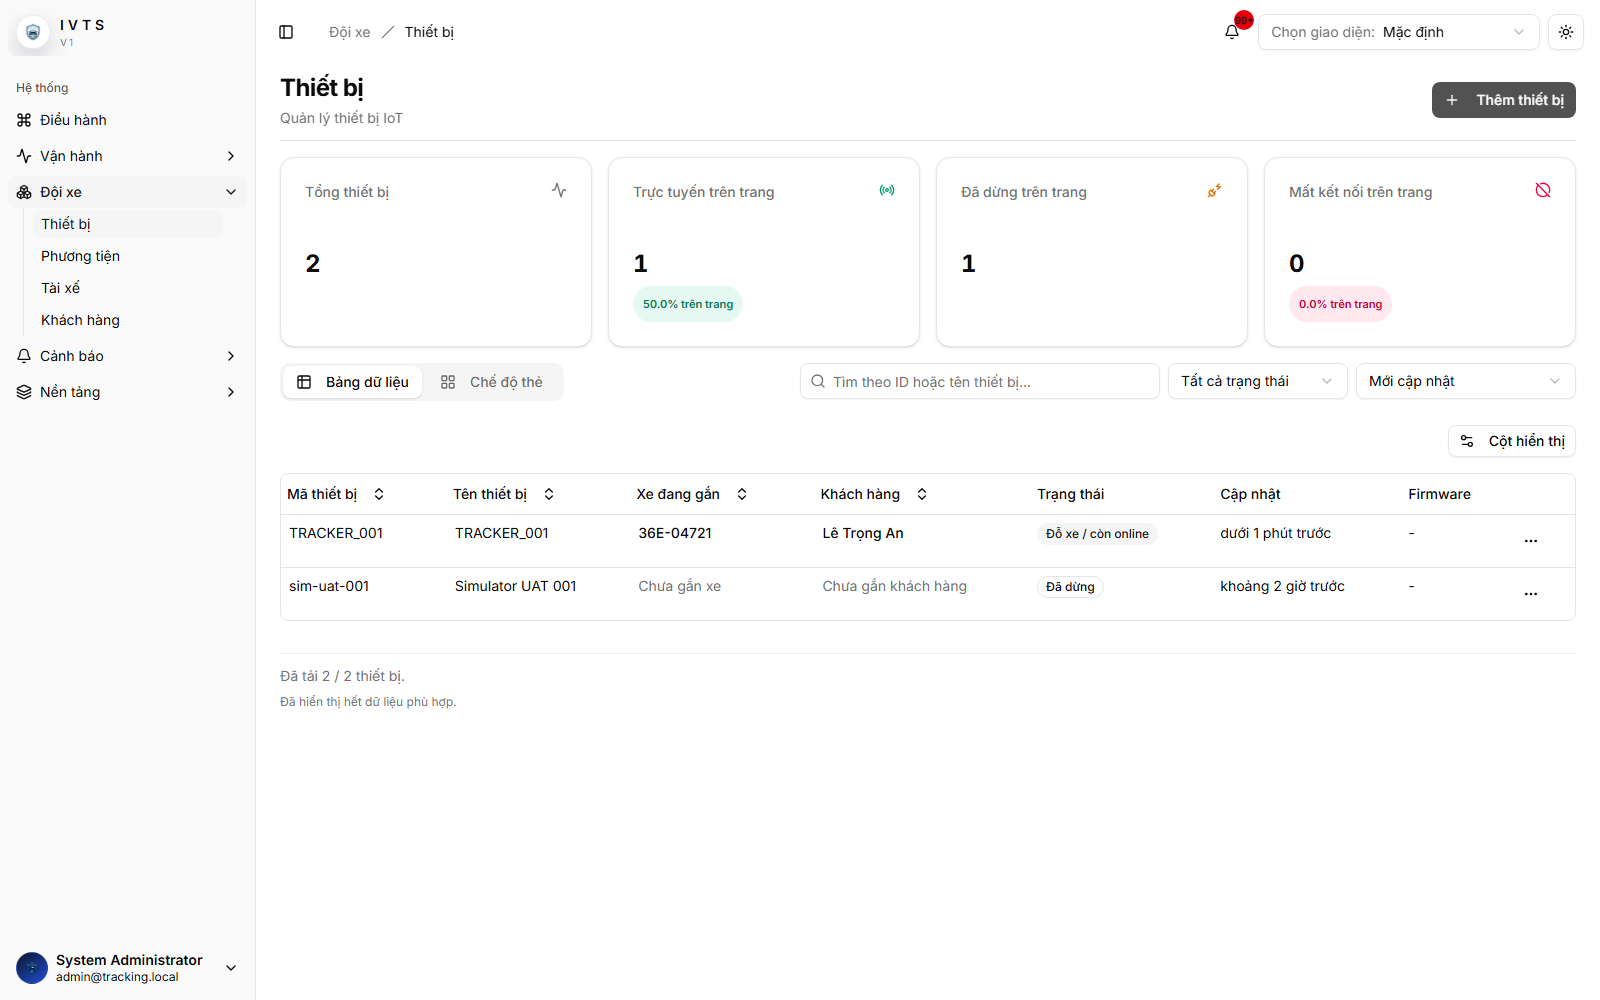
\includegraphics[width=0.96\linewidth,height=0.58\textheight,keepaspectratio]{./assets/result/he-thong-that/03-devices-page.png}
\caption{Giao diện quản lý thiết bị và trạng thái đội xe}
\label{fig:condensed-hinh-4-7-giao-dien-quan-ly-thiet-bi-va-trang-thai-doi-xe}
\end{figure}
}

{\thesissetfigureid{4.8}{condensed-hinh-4-8-giao-dien-ban-do-giam-sat-va-danh-sach-thiet-bi-dang-theo-doi}
\begin{figure}[H]
\centering
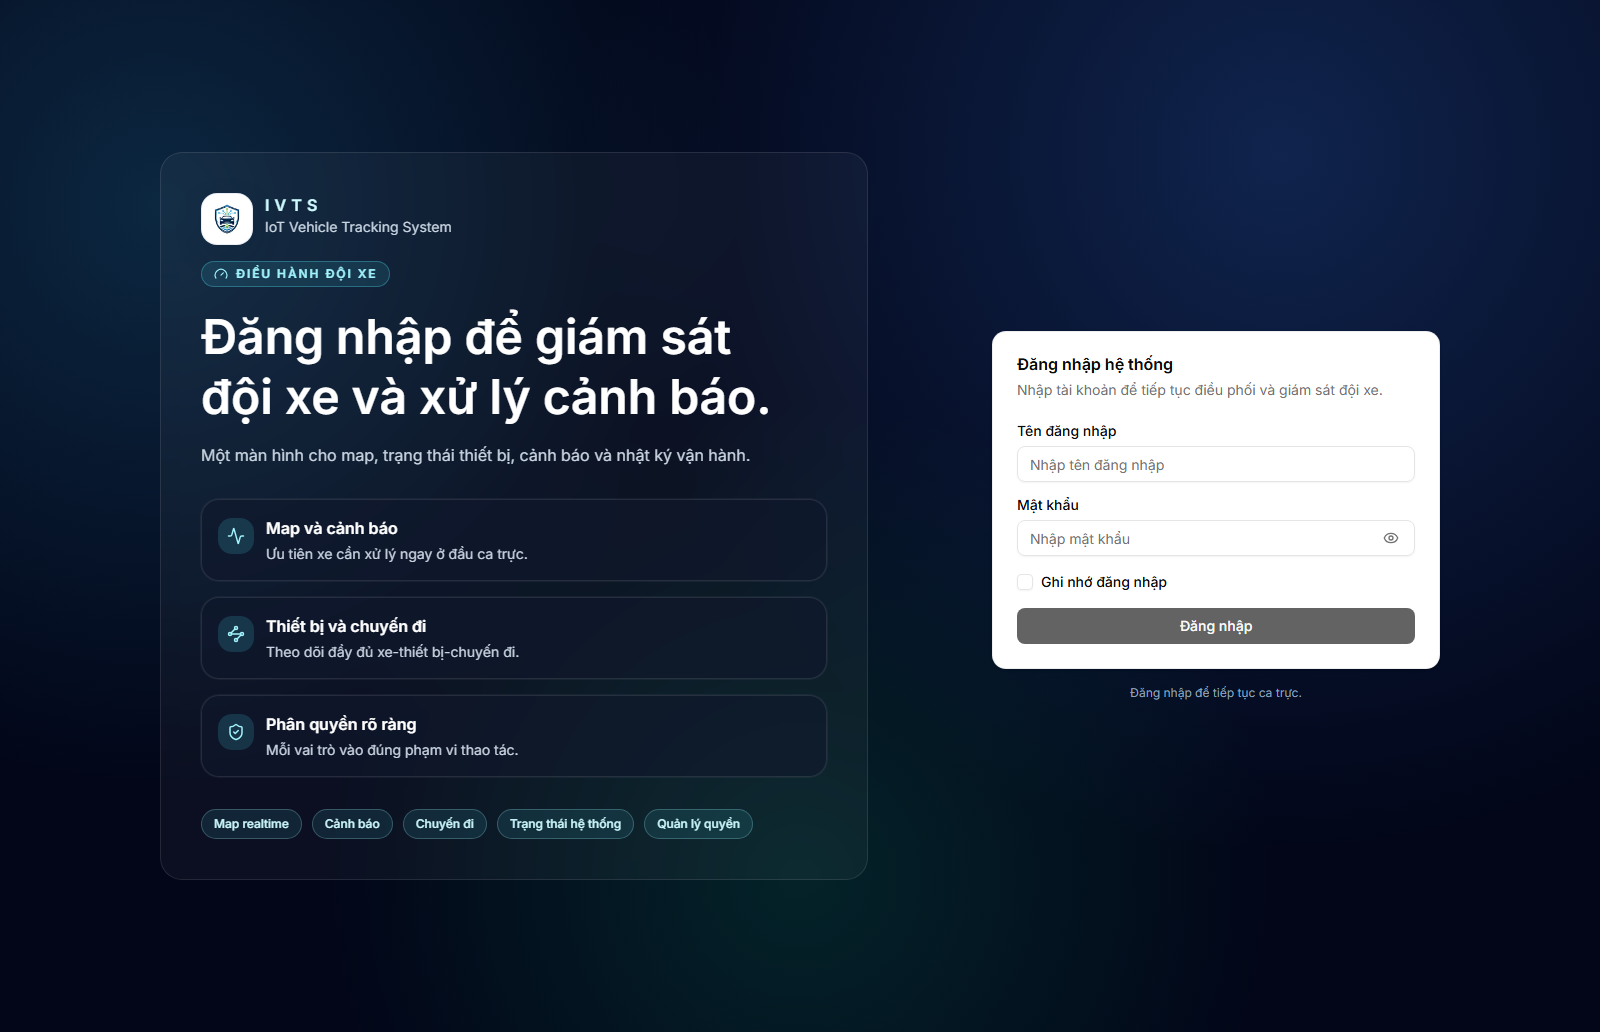
\includegraphics[width=0.96\linewidth,height=0.58\textheight,keepaspectratio]{./assets/result/he-thong-that/01-dashboard-map.png}
\caption{Giao diện bản đồ giám sát và danh sách thiết bị đang theo dõi}
\label{fig:condensed-hinh-4-8-giao-dien-ban-do-giam-sat-va-danh-sach-thiet-bi-dang-theo-doi}
\end{figure}
}

{\thesissetfigureid{4.9}{condensed-hinh-4-9-giao-dien-chi-tiet-thiet-bi-o-tab-du-lieu-tho-obd}
\begin{figure}[H]
\centering
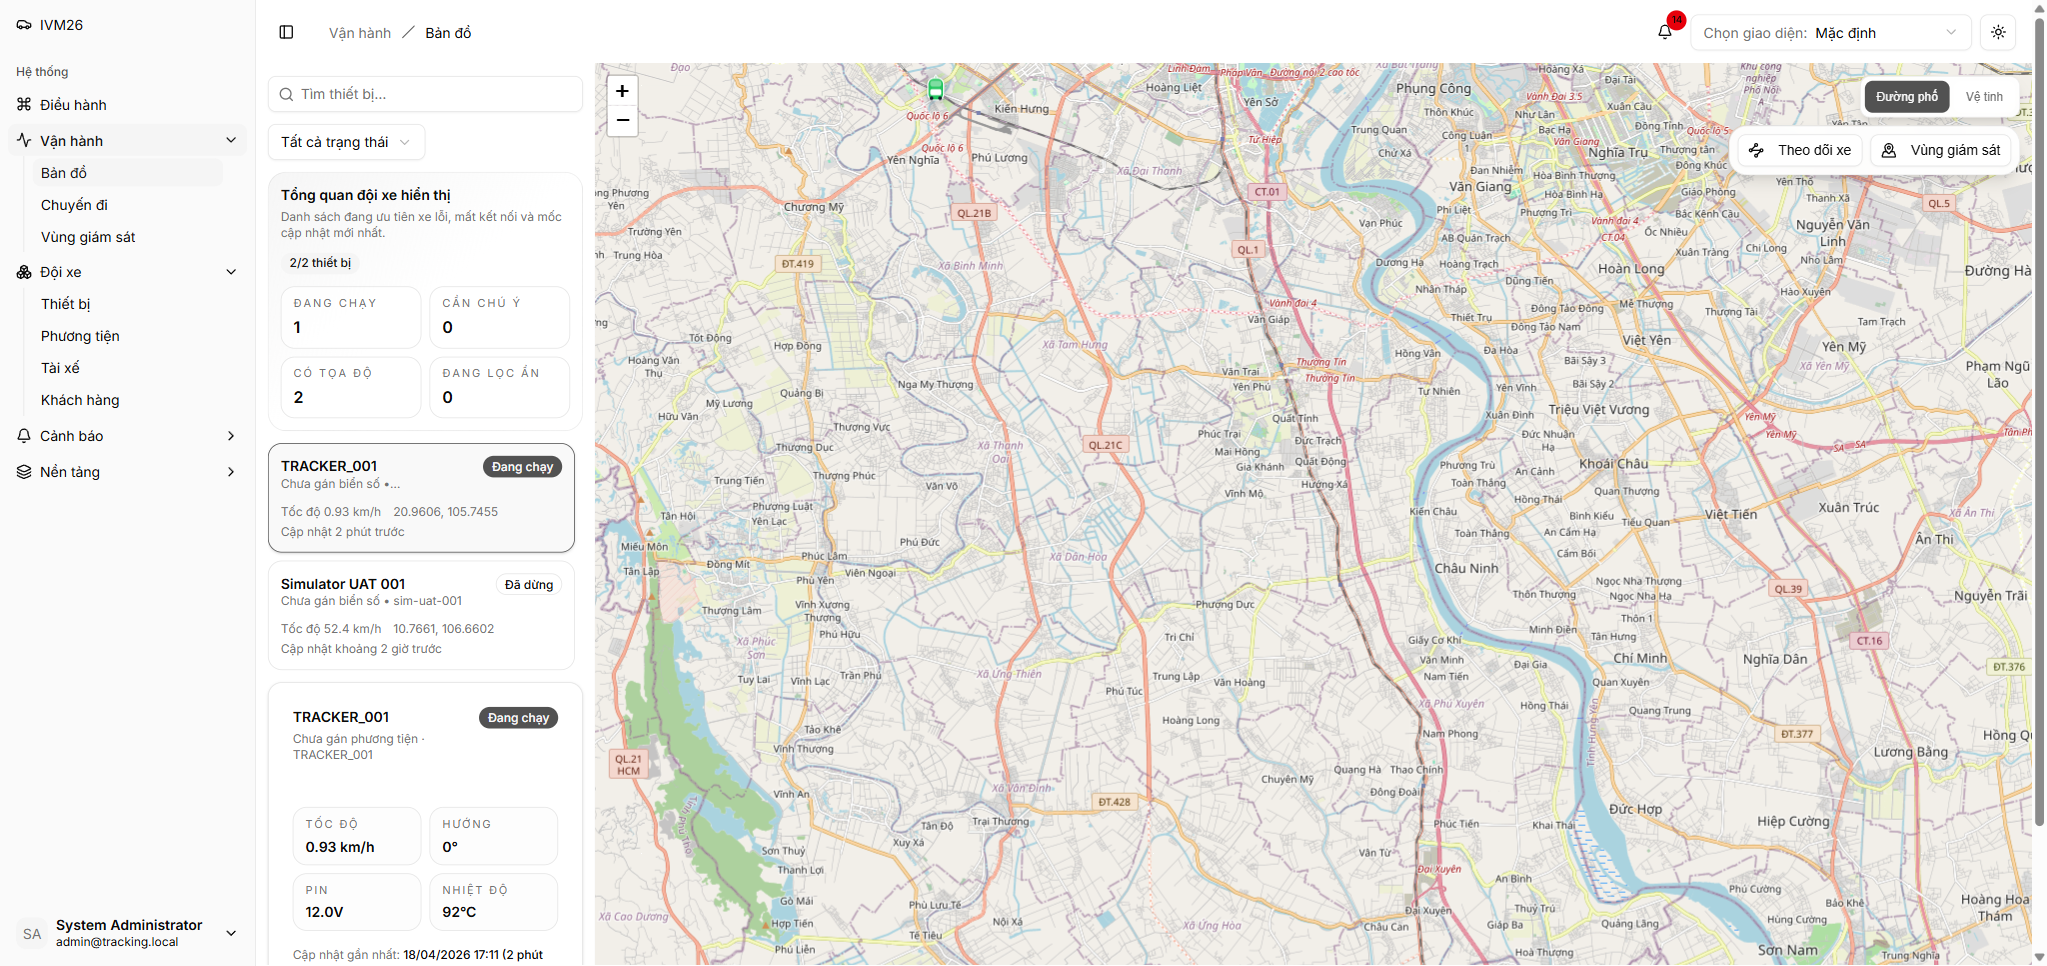
\includegraphics[width=0.96\linewidth,height=0.58\textheight,keepaspectratio]{./assets/result/anh-da-chon-bao-cao/giao-dien-du-lieu-obd-live.png}
\caption{Giao diện chi tiết thiết bị ở tab dữ liệu thô OBD}
\label{fig:condensed-hinh-4-9-giao-dien-chi-tiet-thiet-bi-o-tab-du-lieu-tho-obd}
\end{figure}
}

\subsubsection{4.3.6. Triển khai công khai trên cloud VPS và hướng dẫn dùng thử}\label{triux1ec3n-khai-cuxf4ng-khai-truxean-cloud-vps-vuxe0-hux1b0ux1edbng-dux1eabn-duxf9ng-thux1eed}

Kết quả quan trọng của giai đoạn này là hệ thống đã được công bố trên Internet
thông qua các tên miền riêng thay vì chỉ vận hành trong môi trường cục bộ. Mô
hình truy cập được tổ chức theo tuyến Cloudflare DNS, cloud VPS, lớp chuyển tiếp ngược (reverse proxy)
và các container dịch vụ phía sau. Trong cấu hình hiện tại, frontend, backend,
EMQX, Grafana và lớp quản trị proxy đều có địa chỉ truy cập riêng; riêng
VictoriaMetrics được giữ ở chế độ nội bộ để giảm bề mặt công khai không cần thiết.

{\thesissettableid{4.13}{condensed-bang-4-13-cac-diem-truy-cap-cong-khai-cua-he-thong-tren-cloud-vps}
\def\LTcaptype{table}
\begin{longtable}{|L{0.36\linewidth}|L{0.17\linewidth}|L{0.43\linewidth}|}
\caption{Các điểm truy cập công khai của hệ thống trên cloud VPS}\label{tab:condensed-bang-4-13-cac-diem-truy-cap-cong-khai-cua-he-thong-tren-cloud-vps}\\
\hline
\textbf{Địa chỉ truy cập} & \textbf{Dịch vụ} & \textbf{Vai trò sử dụng} \\
\hline
\endfirsthead
\caption[]{Các điểm truy cập công khai của hệ thống trên cloud VPS (tiếp theo)}\\
\hline
\textbf{Địa chỉ truy cập} & \textbf{Dịch vụ} & \textbf{Vai trò sử dụng} \\
\hline
\endhead
\endfoot
\endlastfoot
\url{https://thingdock.dev} & Frontend & Giao diện web quản trị của hệ thống \\\hline
\url{https://api.thingdock.dev} & Backend & Điểm truy cập REST API \\\hline
\url{https://api.thingdock.dev/api-docs} & Tài liệu API & Giao diện tài liệu API phục vụ kiểm tra các điểm truy cập \\\hline
\url{mqtt.thingdock.dev} & EMQX & Điểm kết nối MQTT của thiết bị \\\hline
\url{https://grafana.thingdock.dev} & Grafana & Quan sát chỉ số và nhật ký vận hành \\\hline
\url{https://emqx.thingdock.dev} & EMQX Dashboard & Quản trị và theo dõi trạng thái broker \\\hline
\url{https://npm.thingdock.dev} & Nginx Proxy Manager & Quản trị lớp chuyển tiếp ngược \\\hline
\end{longtable}
}

Tài khoản mặc định để dùng thử giao diện quản trị được khởi tạo cùng cơ sở dữ
liệu là \thesisterm{admin\ /\ Admin@2026}.

Có thể dùng thử hệ thống theo ba bước ngắn sau:

\begin{enumerate}
\def\labelenumi{\arabic{enumi}.}
\tightlist
\item
  Truy cập \thesisterm{https://thingdock.dev}, đăng nhập bằng tài khoản mặc định \thesisterm{admin\ /\ Admin@2026}.
\item
  Kiểm tra các phân hệ cốt lõi gồm Dashboard, Devices, Map, Alerts và Firmware để đánh giá đầy đủ chuỗi giám sát, cảnh báo và quản trị thiết bị.
\item
  Khi cần kiểm tra lớp API, truy cập \thesisterm{https://api.thingdock.dev/api-docs} để xem danh mục endpoint và mô tả tham số.
\end{enumerate}

\subsection{4.4. Kết quả triển khai và tích hợp toàn hệ thống - Deployment results and integration}\label{kux1ebft-quux1ea3-triux1ec3n-khai-vuxe0-tuxedch-hux1ee3p-touxe0n-hux1ec7-thux1ed1ng---deployment-results-and-integration}

\subsubsection{4.4.1. Mức độ hoàn thành các hạng mục triển khai}\label{mux1ee9c-ux111ux1ed9-houxe0n-thuxe0nh-cuxe1c-hux1ea1ng-mux1ee5c-triux1ec3n-khai}

Kết quả triển khai ở Chương 4 cho thấy toàn bộ các lớp đã được ghép kín thành một
hệ thống hoàn chỉnh, từ phần cứng thiết bị, firmware, tuyến MQTT, lớp lưu trữ,
backend đến frontend công khai trên cloud VPS. Đây là cơ sở để khẳng định đề tài
đã hoàn thành ở mức triển khai thật, không chỉ dừng ở mức mô phỏng hoặc thiết kế
giải pháp.

{\thesissettableid{4.14}{condensed-bang-4-14-muc-do-hoan-thanh-cac-hang-muc-trien-khai-chinh}
\def\LTcaptype{table}
\begin{longtable}{|L{0.207\linewidth}|L{0.621\linewidth}|L{0.13\linewidth}|}
\caption{Mức độ hoàn thành các hạng mục triển khai chính}\label{tab:condensed-bang-4-14-muc-do-hoan-thanh-cac-hang-muc-trien-khai-chinh}\\
\hline
\textbf{Hạng mục} & \textbf{Kết quả chính} & \textbf{Mức độ hoàn thành} \\
\hline
\endfirsthead
\caption[]{Mức độ hoàn thành các hạng mục triển khai chính (tiếp theo)}\\
\hline
\textbf{Hạng mục} & \textbf{Kết quả chính} & \textbf{Mức độ hoàn thành} \\
\hline
\endhead
\endfoot
\endlastfoot
Thiết kế mạch và PCB & Đã hoàn thành sơ đồ nguyên lý, bố trí PCB và hồ sơ phục vụ chế tạo & Hoàn thành \\\hline
Gia công và lắp ráp phần cứng & PCB đã được gia công, linh kiện đã được hàn lắp đầy đủ, hình thành nguyên mẫu thật & Hoàn thành \\\hline
Firmware thiết bị & Đã hiện thực đầy đủ các lớp chức năng và vận hành trên phần cứng thật & Hoàn thành \\\hline
MQTT broker và các lớp lưu trữ & EMQX, PostgreSQL/PostGIS, VictoriaMetrics và VictoriaLogs đã được triển khai & Hoàn thành \\\hline
MQTT Bridge & Đã hiện thực thành dịch vụ độc lập cho tuyến tiếp nhận dữ liệu thiết bị & Hoàn thành \\\hline
Backend & Đã hoàn thành các nhóm API và dịch vụ nghiệp vụ cốt lõi & Hoàn thành \\\hline
Frontend & Đã hoàn thành giao diện quản trị web với các phân hệ chính & Hoàn thành \\\hline
Cloud VPS và tên miền công khai & Hệ thống đã công bố qua \thesisterm{thingdock.dev} và các tên miền dịch vụ liên quan & Hoàn thành \\\hline
Quan sát vận hành & Đã tích hợp Grafana, VictoriaLogs và EMQX Dashboard để hỗ trợ vận hành & Hoàn thành \\\hline
\end{longtable}
}

\subsubsection{4.4.2. Đối chiếu với các chỉ tiêu nghiệm thu}\label{ux111ux1ed1i-chiux1ebfu-vux1edbi-cuxe1c-chux1ec9-tiuxeau-nghiux1ec7m-thu}

Khi đối chiếu với các chỉ tiêu đã xác lập ở Mục 1.3, có thể thấy các yêu cầu cốt
lõi của đề tài đều đã được hiện thực trên hệ thống thật. Kết quả này không chỉ thể
hiện ở từng thành phần riêng lẻ, mà còn ở việc toàn tuyến thiết bị - máy chủ -
giao diện đã vận hành đồng bộ.

{\thesissettableid{4.15}{condensed-bang-4-15-doi-chieu-ket-qua-trien-khai-voi-cac-chi-tieu-dat-ra}
\def\LTcaptype{table}
\begin{longtable}{|L{0.160\linewidth}|L{0.700\linewidth}|L{0.090\linewidth}|}
\caption{Đối chiếu kết quả triển khai với các chỉ tiêu đặt ra}\label{tab:condensed-bang-4-15-doi-chieu-ket-qua-trien-khai-voi-cac-chi-tieu-dat-ra}\\
\hline
\textbf{Nhóm chỉ tiêu} & \textbf{Kết quả đã đạt được} & \textbf{Đánh giá} \\
\hline
\endfirsthead
\caption[]{Đối chiếu kết quả triển khai với các chỉ tiêu đặt ra (tiếp theo)}\\
\hline
\textbf{Nhóm chỉ tiêu} & \textbf{Kết quả đã đạt được} & \textbf{Đánh giá} \\
\hline
\endhead
\endfoot
\endlastfoot
Phần cứng & Đã hoàn thiện thiết kế mạch, PCB chuyên dụng, nguyên mẫu đã gia công và hàn lắp đầy đủ, có thể lắp đặt trên xe thật & Đạt \\\hline
Firmware & Đã thu thập dữ liệu GNSS, dữ liệu OBD cơ bản, giám sát nguồn, quản lý trạng thái, lưu đệm ngoại tuyến và hỗ trợ OTA & Đạt \\\hline
Máy chủ và xử lý dữ liệu & Đã tiếp nhận dữ liệu liên tục qua MQTT, phân vai lưu trữ theo bản chất dữ liệu và cung cấp lớp dịch vụ quản trị tập trung & Đạt \\\hline
Giao diện web & Đã cung cấp dashboard, bản đồ, giám sát thiết bị, cảnh báo, quản lý đội xe và quản trị nền tảng qua trình duyệt web & Đạt \\\hline
Tích hợp toàn tuyến & Đã hình thành chuỗi thiết bị - EMQX - MQTT Bridge - lưu trữ - backend - frontend vận hành thống nhất & Đạt \\\hline
\end{longtable}
}

\subsubsection{4.4.3. Kết luận chương 4}\label{kux1ebft-luux1eadn-chux1b0ux1a1ng-4}

Như vậy, các phương án đã lựa chọn ở Chương 3 đã được hiện thực thành một hệ
thống hoàn chỉnh và vận hành được trên hạ tầng thật. Phần cứng đã đi từ sơ đồ
thiết kế tới PCB đã gia công và lắp ráp; firmware đã được triển khai đầy đủ trên
thiết bị; còn hệ thống cloud đã được đưa lên cloud VPS với các dịch vụ và tên
miền công khai. Kết quả này xác nhận đề tài đã hoàn thành trọn vẹn chuỗi thiết bị đến máy chủ - giao diện trong phạm vi mục tiêu đặt ra.

\chapterheading{CHƯƠNG 5. ĐÁNH GIÁ VÀ KHUYẾN NGHỊ -- EVALUATION AND RECOMMENDATIONS}

\subsection{5.1. Đánh giá hiệu năng}\label{ux111uxe1nh-giuxe1-hiux1ec7u-nux103ng}

\subsubsection{5.1.1. Đánh giá chung}\label{ux111uxe1nh-giuxe1-chung}

Kết quả ở Chương 4 cho thấy nguyên mẫu đã đạt mục tiêu của một hệ thống IoT
quản lý phương tiện ở mức nguyên mẫu tích hợp. Kết quả sẽ được đánh giá trước hết theo khả năng đáp ứng chức năng, độ ổn
định qua các phiên kiểm chứng và khả năng duy trì kiến trúc phân lớp khi tích
hợp toàn tuyến.

{\thesissettableid{5.1}{condensed-bang-5-1-danh-gia-hieu-nang-theo-nhom-chuc-nang}
\def\LTcaptype{table}
\begin{longtable}{|L{0.122\linewidth}|L{0.494\linewidth}|L{0.342\linewidth}|}
\caption{Đánh giá hiệu năng theo nhóm chức năng}\label{tab:condensed-bang-5-1-danh-gia-hieu-nang-theo-nhom-chuc-nang}\\
\hline
\textbf{Nhóm chức năng} & \textbf{Mức đáp ứng hiện tại} & \textbf{Giới hạn còn lại} \\
\hline
\endfirsthead
\caption[]{Đánh giá hiệu năng theo nhóm chức năng (tiếp theo)}\\
\hline
\textbf{Nhóm chức năng} & \textbf{Mức đáp ứng hiện tại} & \textbf{Giới hạn còn lại} \\
\hline
\endhead
\endfoot
\endlastfoot
Phần cứng thiết bị & Nguyên mẫu phần cứng đã tích hợp đủ khối xử lý, truyền thông, cảm biến, lưu đệm cục bộ và nguồn dự phòng & Cần kiểm chứng thêm về nhiễu, nhiệt và độ bền cơ khí khi lắp dài ngày \\\hline
Nguồn và năng lượng & Đã tách nhánh modem, đo điện áp và áp dụng cơ chế ngủ sâu theo trạng thái xe & Cần đo thêm trên nhiều loại ắc quy và nhiều chu kỳ đỗ dài \\\hline
Firmware & Đã điều phối được trạng thái chạy, đỗ, cảnh báo, truyền dữ liệu và cập nhật từ xa & Cần tối ưu thêm trong các tình huống mất mạng kéo dài hoặc BLE OBD2 dao động \\\hline
Thu nhận dữ liệu xe & Đã đọc được OBD2 cơ bản, trạng thái nguồn, vị trí GNSS và chuyển động bất thường & Chưa mở rộng toàn bộ mã lỗi DTC và các thông số chuyên sâu \\\hline
Kết nối thiết bị - máy chủ & MQTT đáp ứng tốt bản tin nhỏ, chu kỳ lặp và sự kiện ưu tiên & Cần kiểm thử thêm ở vùng sóng yếu và khi số thiết bị tăng \\\hline
Máy chủ và giao diện & Đã nhận, lưu và hiển thị được vị trí, trạng thái, cảnh báo và lịch sử & Cần đánh giá sâu hơn về tải đồng thời và độ trễ khi mở rộng quy mô \\\hline
\end{longtable}
}

\subsubsection{5.1.2. Nhận xét theo yêu cầu thiết kế}\label{nhux1eadn-xuxe9t-theo-yuxeau-cux1ea7u-thiux1ebft-kux1ebf}

Xét theo yêu cầu thiết kế ở Chương 2, nguyên mẫu đã đáp ứng rõ ba nhóm mục tiêu
chính. Thứ nhất, hệ thống đã chuyển được dữ liệu từ xe thành thông tin quản trị
trên giao diện web, gồm vị trí, trạng thái thiết bị, lịch sử và cảnh báo. Thứ
hai, thiết bị đã có cơ chế quản lý nguồn phù hợp với bối cảnh lắp trên xe, nhờ
đó giảm rủi ro tiêu thụ điện không kiểm soát khi xe đỗ. Thứ ba, kiến trúc nhiều
lớp đã chứng minh được tính đúng về mặt tổ chức, khi dữ liệu được tiếp nhận,
phân vai lưu trữ và khai thác tập trung.

Những nội dung hiện mới được xác nhận ở mức nguyên mẫu gồm độ bền dài ngày, mức
ổn định trên nhiều mẫu xe, phạm vi tương thích OBD2 mở rộng và khả năng vận
hành khi số lượng thiết bị tăng cao. Do đó, có thể kết luận rằng phương án lựa
chọn là đúng về cấu trúc và đủ cho mục tiêu đồ án, nhưng chưa phải là kết quả
đủ để suy rộng trực tiếp sang triển khai thương mại quy mô lớn.

\subsection{5.2. Đánh giá kinh tế và môi trường}\label{ux111uxe1nh-giuxe1-kinh-tux1ebf-vuxe0-muxf4i-trux1b0ux1eddng}

\subsubsection{5.2.1. Đánh giá kinh tế}\label{ux111uxe1nh-giuxe1-kinh-tux1ebf}

Về mặt kinh tế, chi phí của hệ thống được tách thành hai nhóm chính: chi phí chế
tạo thiết bị và chi phí vận hành hằng năm. Trong đó, chi phí chế tạo mỗi thiết bị
được lấy theo BOM ước tính của thiết bị; còn chi phí vận hành gồm chi phí kết nối dữ liệu di động
cho từng thiết bị và chi phí hạ tầng dùng chung ở phía máy chủ.

{\thesissettableid{5.2}{condensed-bang-5-2-cau-phan-chi-phi-chinh-cua-he-thong}
\def\LTcaptype{table}
\begin{longtable}{|L{0.085\linewidth}|L{0.429\linewidth}|L{0.151\linewidth}|L{0.08\linewidth}|L{0.199\linewidth}|}
\caption{Cấu phần chi phí chính của hệ thống}\label{tab:condensed-bang-5-2-cau-phan-chi-phi-chinh-cua-he-thong}\\
\hline
\textbf{Hạng mục chi phí} & \textbf{Cách tính và thông số chính} & \textbf{Mức chi phí} & \textbf{Phạm vi áp dụng} & \textbf{Nhận xét} \\
\hline
\endfirsthead
\caption[]{Cấu phần chi phí chính của hệ thống (tiếp theo)}\\
\hline
\textbf{Hạng mục chi phí} & \textbf{Cách tính và thông số chính} & \textbf{Mức chi phí} & \textbf{Phạm vi áp dụng} & \textbf{Nhận xét} \\
\hline
\endhead
\endfoot
\endlastfoot
Thiết bị phần cứng & Theo BOM ước tính của thiết bị & Khoảng 1.500.000 VND cho mỗi thiết bị (theo BOM) & Từng thiết bị & Là khoản đầu tư ban đầu lớn nhất của hệ thống \\\hline
Kết nối dữ liệu di động & Gói Viettel NB-IoT Connect8, cước 8.000 VND/30 ngày, tốc độ danh nghĩa khoảng 50 Kbps chiều lên và 50 Kbps chiều xuống & Khoảng 96.000 VND/năm cho mỗi thiết bị & Từng thiết bị & Phù hợp với bản tin telemetry dung lượng nhỏ, gửi theo chu kỳ \\\hline
Máy chủ VPS trên đám mây & Một VPS cấu hình cơ bản để chạy broker MQTT, MQTT Bridge, backend, frontend và các dịch vụ quan sát vận hành của mô hình thử nghiệm & Khoảng 500.000-900.000 VND/năm & Dùng chung toàn hệ thống & Phù hợp với quy mô đồ án và giai đoạn thử nghiệm \\\hline
Tên miền & Một tên miền chính, dùng thêm các tên miền phụ cho web, API, MQTT và giám sát & Khoảng 200.000-300.000 VND/năm & Dùng chung toàn hệ thống & Không làm tăng theo số lượng thiết bị \\\hline
\end{longtable}
}

Với cách tính trên, chi phí vận hành bình quân hằng năm cho mỗi thiết bị gồm
khoảng 96.000 VND tiền kết nối dữ liệu, cộng với phần chi phí hạ tầng dùng chung
được phân bổ theo số lượng thiết bị triển khai. Nếu gọi \(n\) là số thiết bị đang
vận hành, thì phần chi phí dùng chung bình quân trên mỗi thiết bị xấp xỉ
\((700.000-1.200.000)/n\) VND/năm, trong đó máy chủ VPS và tên miền đã được tách
riêng như trong Bảng 5.2. Như vậy, chi phí năm đầu cho mỗi thiết bị sẽ bằng chi
phí chế tạo thiết bị cộng với 96.000 VND và phần hạ tầng phân bổ; từ các
năm tiếp theo, chi phí duy trì chủ yếu còn lại là tiền kết nối dữ liệu và phần
chi phí máy chủ dùng chung.

Xét theo mục tiêu của đồ án, cấu hình chi phí này là hợp lý vì vẫn đủ để triển
khai thực tết cho doanh nghiệp một hệ thống hoàn chỉnh từ thiết bị, truyền dữ liệu, lưu trữ tới giao diện
quản trị trên cloud VPS, nhưng không đòi hỏi mức đầu tư vận hành lớn. Khi số
lượng thiết bị tăng, phần chi phí VPS và tên miền phân bổ trên mỗi thiết bị giảm
dần; do đó hiệu quả kinh tế của mô hình sẽ rõ hơn ở quy mô triển khai nhiều
thiết bị.

\subsubsection{5.2.2. Đánh giá môi trường}\label{ux111uxe1nh-giuxe1-muxf4i-trux1b0ux1eddng}

Ở góc độ môi trường, hệ thống có thể tạo ra tác động tích cực thông qua việc hỗ
trợ theo dõi hành trình, kiểm soát sử dụng phương tiện và phát hiện sớm các dấu
hiệu cần bảo trì. Nếu được khai thác đúng mục đích, dữ liệu thu được có thể
giúp giảm sử dụng xe ngoài phạm vi cho phép, giảm hao mòn không được theo dõi
và nâng cao hiệu quả vận hành đội xe.

Ở chiều ngược lại, thiết bị điện tử, pin dự phòng và phụ kiện lắp đặt đều tạo ra
nguy cơ phát sinh chất thải điện tử nếu thay thế không đúng quy trình. Do đó,
hướng phát triển tiếp theo cần ưu tiên các giải pháp cơ khí bền hơn, pin có
nguồn gốc rõ ràng, thiết kế dễ tháo lắp và quy trình thu hồi linh kiện hỏng khi
chuyển từ nguyên mẫu sang triển khai thử nghiệm thực tế.

\subsection{5.3. Đánh giá rủi ro và biện pháp giảm thiểu}\label{ux111uxe1nh-giuxe1-rux1ee7i-ro-vuxe0-biux1ec7n-phuxe1p-giux1ea3m-thiux1ec3u}

Phần đánh giá rủi ro tập trung vào những điểm có thể ảnh hưởng trực tiếp đến độ
tin cậy của hệ thống khi chuyển từ nguyên mẫu trong phòng thí nghiệm sang vận
hành ngoài hiện trường. Đây là các rủi ro có khả năng tác động đồng thời lên
thiết bị, đường truyền và lớp khai thác.

{\thesissettableid{5.3}{condensed-bang-5-3-rui-ro-ky-thuat-va-bien-phap-giam-thieu}
\def\LTcaptype{table}
\begin{longtable}{|L{0.150\linewidth}|L{0.115\linewidth}|L{0.340\linewidth}|L{0.345\linewidth}|}
\caption{Rủi ro kỹ thuật và biện pháp giảm thiểu}\label{tab:condensed-bang-5-3-rui-ro-ky-thuat-va-bien-phap-giam-thieu}\\
\hline
\textbf{Rủi ro} & \textbf{Mức ảnh hưởng} & \textbf{Biện pháp đã áp dụng} & \textbf{Hướng giảm thiểu tiếp theo} \\
\hline
\endfirsthead
\caption[]{Rủi ro kỹ thuật và biện pháp giảm thiểu (tiếp theo)}\\
\hline
\textbf{Rủi ro} & \textbf{Mức ảnh hưởng} & \textbf{Biện pháp đã áp dụng} & \textbf{Hướng giảm thiểu tiếp theo} \\
\hline
\endhead
\endfoot
\endlastfoot
Sụt áp khi modem truyền dữ liệu & Cao & Tách nhánh nguồn modem và logic, theo dõi điện áp bằng ADC & Đo dao động nguồn ở nhiều kịch bản tải và hoàn thiện thêm lớp bảo vệ \\\hline
Hao ắc quy khi xe đỗ lâu & Cao & Dùng ngủ sâu, theo dõi điện áp và tắt bớt tải theo trạng thái & Kiểm thử dài ngày trên nhiều xe và nhiều điều kiện sử dụng \\\hline
Thiết bị bị tháo khỏi xe & Cao & Phát hiện mất nguồn chính, chuyển sang pin dự phòng và gửi cảnh báo ngay về máy chủ & Bổ sung thêm cơ chế phát hiện tháo gỡ chuyên dụng để giảm báo động giả \\\hline
Bộ chuyển đổi OBD2 bị rút & Trung bình - cao & Khi thiết bị vẫn còn pin dự phòng, hệ thống vẫn có thể phát cảnh báo mất kết nối OBD2 về máy chủ & Đối chiếu thêm phiên kết nối OBD2 và trạng thái vận hành để tăng độ tin cậy cảnh báo \\\hline
Mất sóng di động hoặc sóng yếu & Trung bình - cao & Phục hồi kết nối, phát lại dữ liệu chờ và phân mức QoS theo loại bản tin & Tăng thời gian thử ở vùng phủ sóng kém và tối ưu chiến lược gửi \\\hline
Kết nối OBD2 BLE không ổn định & Trung bình & Tự kết nối lại bộ chuyển đổi và tách luồng OBD2 khỏi lõi điều phối & Chuẩn hóa thêm danh sách bộ chuyển đổi tương thích \\\hline
Sai lệch vị trí GNSS & Trung bình & Ghi nhận vị trí theo phiên vận hành và đối chiếu hành trình & Bổ sung thêm kiểm chứng ở khu vực đô thị dày đặc và điểm che khuất \\\hline
Lộ dữ liệu vị trí & Cao & Xác thực và phân quyền ở lớp quản trị & Hoàn thiện mã hóa đường truyền, chính sách lưu dữ liệu và quyền truy cập \\\hline
Lỗi cập nhật firmware từ xa & Cao & Chỉ cho phép cập nhật khi đủ điều kiện nguồn và kết nối & Bổ sung cơ chế quay lại phiên bản trước nếu cập nhật không thành công \\\hline
\end{longtable}
}

Như vậy, các rủi ro chính của hệ thống không nằm ở một lớp đơn lẻ, mà trải dài
từ phần cứng, kết nối di động tới dữ liệu và vận hành. Điều này cũng củng cố lựa
chọn kiến trúc phân lớp ở Chương 3, vì mỗi rủi ro cần được khoanh vùng và xử lý
ở đúng lớp chịu trách nhiệm.

\subsection{5.4. Khuyến nghị cho tương lai}\label{khuyux1ebfn-nghux1ecb-cho-tux1b0ux1a1ng-lai}

Trên cơ sở kết quả hiện tại, các hướng phát triển tiếp theo nên được sắp xếp
theo mức độ ảnh hưởng đến khả năng chuyển từ nguyên mẫu sang thử nghiệm thực tế.

{\thesissettableid{5.4}{condensed-bang-5-4-huong-khuyen-nghi-cho-giai-doan-tiep-theo}
\def\LTcaptype{table}
\begin{longtable}{|L{0.077\linewidth}|L{0.342\linewidth}|L{0.54\linewidth}|}
\caption{Hướng khuyến nghị cho giai đoạn tiếp theo}\label{tab:condensed-bang-5-4-huong-khuyen-nghi-cho-giai-doan-tiep-theo}\\
\hline
\textbf{Mức ưu tiên} & \textbf{Hướng phát triển} & \textbf{Mục tiêu chính} \\
\hline
\endfirsthead
\caption[]{Hướng khuyến nghị cho giai đoạn tiếp theo (tiếp theo)}\\
\hline
\textbf{Mức ưu tiên} & \textbf{Hướng phát triển} & \textbf{Mục tiêu chính} \\
\hline
\endhead
\endfoot
\endlastfoot
Cao & Kiểm thử thực địa dài ngày trên nhiều xe & Xác nhận độ ổn định của nguồn, GNSS, 4G và luồng cảnh báo trong điều kiện thật \\\hline
Cao & Hoàn thiện vỏ và quy trình lắp đặt & Giảm rủi ro cơ khí, rủi ro đấu nối và tăng tính lặp lại khi triển khai \\\hline
Cao & Tăng an toàn dữ liệu và quyền riêng tư & Hoàn thiện mã hóa đường truyền, phân quyền và chính sách lưu giữ dữ liệu vị trí \\\hline
Trung bình & Mở rộng dữ liệu OBD2 và chẩn đoán & Bổ sung giá trị cho theo dõi bảo trì và phân tích tình trạng xe \\\hline
Trung bình & Tối ưu năng lượng theo trạng thái xe & Kéo dài khả năng giám sát khi xe đỗ lâu và giảm ảnh hưởng đến ắc quy \\\hline
Trung bình & Chuẩn hóa vận hành thử nghiệm và bảo trì & Hình thành checklist lắp đặt, kiểm tra sau lắp và tài liệu hỗ trợ bảo trì \\\hline
Dài hạn & Mở rộng kênh khai thác phụ trợ như ứng dụng di động & Bổ sung cảnh báo nhanh và tăng tính linh hoạt khi người quản lý không dùng máy tính \\\hline
\end{longtable}
}

Các khuyến nghị trên cho thấy hướng phát triển hợp lý của hệ thống không phải là
mở rộng tính năng bằng mọi giá, mà là củng cố dần các lớp có tác động lớn nhất
đến độ tin cậy, an toàn dữ liệu và khả năng vận hành thực tế.

\chapterheading{CHƯƠNG 6. PHẢN HỒI VÀ BÀI HỌC KINH NGHIỆM -- REFLECTION AND LESSONS LEARNED}

\subsection{6.1. Ứng dụng kiến thức kỹ thuật - Application of prior coursework}\label{ux1ee9ng-dux1ee5ng-kiux1ebfn-thux1ee9c-kux1ef9-thuux1eadt---application-of-prior-coursework}

Đồ án là sự kết hợp của nhiều mảng kiến thức trong chương trình đào tạo Kỹ thuật
Cơ điện tử. Thay vì chỉ áp dụng một khối kiến thức riêng lẻ, quá trình thực hiện
đòi hỏi sự phối hợp đồng thời giữa thiết kế phần cứng, lập trình hệ thống nhúng,
truyền thông dữ liệu, tổ chức phần mềm máy chủ và kiểm chứng hệ thống.

{\thesissettableid{6.1}{condensed-bang-6-1-kien-thuc-da-ap-dung-trong-do-an}
\def\LTcaptype{table}
\begin{longtable}{|L{0.302\linewidth}|L{0.658\linewidth}|}
\caption{Kiến thức đã áp dụng trong đồ án}\label{tab:condensed-bang-6-1-kien-thuc-da-ap-dung-trong-do-an}\\
\hline
\textbf{Nhóm kiến thức} & \textbf{Ứng dụng trong đồ án} \\
\hline
\endfirsthead
\caption[]{Kiến thức đã áp dụng trong đồ án (tiếp theo)}\\
\hline
\textbf{Nhóm kiến thức} & \textbf{Ứng dụng trong đồ án} \\
\hline
\endhead
\endfoot
\endlastfoot
Mạch điện tử và nguồn & Thiết kế nhánh nguồn, chọn linh kiện hạ áp, bảo vệ nguồn và đo điện áp giám sát \\\hline
Vi điều khiển và hệ nhúng & Điều khiển ESP32-S3, tổ chức tác vụ, giao tiếp UART, I2C, BLE và chế độ ngủ sâu \\\hline
Cảm biến và đo lường & Đọc gia tốc, phát hiện chuyển động bất thường và đối chiếu tín hiệu trong quá trình thử \\\hline
Truyền thông và mạng & Gửi dữ liệu qua 4G/LTE, MQTT, HTTP/REST và cập nhật gần thời gian thực \\\hline
Cơ sở dữ liệu và phần mềm ứng dụng & Tổ chức dữ liệu nghiệp vụ, dữ liệu chuỗi thời gian, nhật ký và giao diện quản trị \\\hline
Kiểm thử, vận hành~và tích hợp hệ thống & Đối chiếu từng lớp với chỉ tiêu nghiệm thu và xác nhận luồng dữ liệu toàn tuyến \\\hline
\end{longtable}
}

Kết quả đạt được cho thấy các học phần nền tảng không tồn tại tách rời nhau trong
một bài toán thực tế. Chỉ khi được ghép lại theo một chuỗi nhất quán, chúng mới
tạo thành một nguyên mẫu có thể vận hành được từ thiết bị đến giao diện quản trị.

\subsection{6.2. Giải quyết các vấn đề kỹ thuật phức tạp - Complex engineering problems}\label{giux1ea3i-quyux1ebft-cuxe1c-vux1ea5n-ux111ux1ec1-kux1ef9-thuux1eadt-phux1ee9c-tux1ea1p---complex-engineering-problems}

Khó khăn lớn nhất của đề tài nằm ở tính phụ thuộc chéo giữa các lớp. Một sai lệch
ở phần nguồn có thể làm kết quả firmware không còn đáng tin cậy; một điểm nghẽn
ở đường truyền có thể khiến giao diện phản ánh sai trạng thái thiết bị; một cách
tổ chức lưu trữ chưa hợp lý có thể làm dữ liệu khó khai thác dù bản tin vẫn được
nhận đầy đủ. Vì vậy, cách tiếp cận phù hợp không phải là tối ưu từng khối riêng
lẻ, mà là giải bài toán ở cấp hệ thống.

{\thesissettableid{6.2}{condensed-bang-6-2-van-de-ky-thuat-va-cach-xu-ly}
\def\LTcaptype{table}
\begin{longtable}{|L{0.256\linewidth}|L{0.414\linewidth}|L{0.288\linewidth}|}
\caption{Vấn đề kỹ thuật và cách xử lý}\label{tab:condensed-bang-6-2-van-de-ky-thuat-va-cach-xu-ly}\\
\hline
\textbf{Vấn đề kỹ thuật} & \textbf{Cách xử lý trong đồ án} & \textbf{Bài học rút ra} \\
\hline
\endfirsthead
\caption[]{Vấn đề kỹ thuật và cách xử lý (tiếp theo)}\\
\hline
\textbf{Vấn đề kỹ thuật} & \textbf{Cách xử lý trong đồ án} & \textbf{Bài học rút ra} \\
\hline
\endhead
\endfoot
\endlastfoot
Mạch PCB phức tạp, yêu cầu nhiều tính năng và phải nhỏ gọn & Phân tách theo các khối nguồn, xử lý, modem, cảm biến và chốt ánh xạ chân ngay từ giai đoạn sơ đồ - PCB & Với thiết bị gắn trên xe, bài toán bố trí và tích hợp mạch quan trọng không kém lựa chọn linh kiện \\\hline
Nhiều trạng thái vận hành từ trạng thái thiết bị, trạng thái di chuyển và trạng thái OBD & Tổ chức máy trạng thái trung tâm, kết hợp trạng thái nguồn, chuyển động và OBD để quyết định chu kỳ lấy mẫu, chế độ ngủ và bản tin gửi đi & Với hệ nhúng trên xe, tối ưu năng lượng phải đi cùng với mô hình trạng thái đủ chặt chẽ \\\hline
Cần lắp trên nhiều xe với ít xâm lấn & Dùng bộ chuyển đổi OBD2 BLE thay cho đấu dây trực tiếp & Tính cơ động khi lắp đặt là một tiêu chí kỹ thuật quan trọng, không chỉ là tiện ích phụ \\\hline
Mạng di động không ổn định & Dùng MQTT, cơ chế kết nối lại và hàng đợi ngoại tuyến & Hệ thống thực tế phải chấp nhận gián đoạn kết nối như một điều kiện bình thường \\\hline
Dữ liệu có bản chất khác nhau & Tách dữ liệu nghiệp vụ, dữ liệu đo từ xa và nhật ký vận hành & Tổ chức lưu trữ quyết định trực tiếp khả năng khai thác và khoanh vùng lỗi \\\hline
Giao diện phục vụ người vận hành & Chuyển dữ liệu kỹ thuật thành bản đồ, trạng thái, cảnh báo và lịch sử & Lớp hiển thị phải phục vụ quyết định vận hành, không chỉ trình bày dữ liệu thô \\\hline
\end{longtable}
}

Như vậy, vấn đề kỹ thuật phức tạp nhất của đồ án không nằm ở một linh kiện hay
một thuật toán riêng lẻ, mà nằm ở việc làm cho nhiều lớp kỹ thuật khác nhau có
thể phối hợp ổn định trong cùng một hệ thống.

\subsection{6.3. Tác động đạo đức và xã hội - Ethical and social impacts}\label{tuxe1c-ux111ux1ed9ng-ux111ux1ea1o-ux111ux1ee9c-vuxe0-xuxe3-hux1ed9i---ethical-and-social-impacts}

Hệ thống giám sát phương tiện có giá trị rõ ràng đối với doanh nghiệp cho thuê xe,
nhưng cũng liên quan trực tiếp đến dữ liệu vị trí và hành trình của người sử dụng.
Vì vậy, các khía cạnh đạo đức và xã hội cần được xem như một phần của thiết kế,
không phải là nội dung bổ sung sau khi hệ thống đã hoàn thiện kỹ thuật.

{\thesissettableid{6.3}{condensed-bang-6-3-cac-khia-canh-dao-duc-va-xa-hoi-can-chu-y}
\def\LTcaptype{table}
\begin{longtable}{|L{0.172\linewidth}|L{0.353\linewidth}|L{0.434\linewidth}|}
\caption{Các khía cạnh đạo đức và xã hội cần chú ý}\label{tab:condensed-bang-6-3-cac-khia-canh-dao-duc-va-xa-hoi-can-chu-y}\\
\hline
\textbf{Khía cạnh} & \textbf{Giá trị tích cực} & \textbf{Yêu cầu kiểm soát} \\
\hline
\endfirsthead
\caption[]{Các khía cạnh đạo đức và xã hội cần chú ý (tiếp theo)}\\
\hline
\textbf{Khía cạnh} & \textbf{Giá trị tích cực} & \textbf{Yêu cầu kiểm soát} \\
\hline
\endhead
\endfoot
\endlastfoot
Quyền riêng tư dữ liệu vị trí & Giúp quản lý xe, đối chiếu hành trình và hỗ trợ xử lý sự cố & Phải giới hạn mục đích sử dụng, thời gian lưu và phạm vi truy cập \\\hline
An toàn khi lắp đặt trên xe & Thiết bị hỗ trợ giám sát mà không can thiệp điều khiển xe & Cần bảo đảm đấu nối, cầu chì và vị trí lắp không làm phát sinh rủi ro mới \\\hline
Minh bạch với người sử dụng xe & Giảm tranh chấp khi có dữ liệu đối chiếu rõ ràng & Cần thông báo rõ việc thu thập dữ liệu và phạm vi sử dụng hợp lệ \\\hline
Bảo mật hệ thống & Hạn chế mất dữ liệu và truy cập trái phép & Phải tăng cường xác thực, phân quyền và bảo vệ đường truyền \\\hline
Trách nhiệm vận hành & Hỗ trợ phát hiện sớm bất thường và hỗ trợ bảo trì & Cần quy định rõ cách xử lý cảnh báo sai hoặc dữ liệu thiếu \\\hline
\end{longtable}
}

Trong phạm vi đồ án, thiết bị chỉ dừng ở mức giám sát, cảnh báo và hỗ trợ ra
quyết định; không can thiệp trực tiếp vào hệ thống điều khiển của xe. Cách tiếp
cận này phù hợp với giai đoạn nguyên mẫu vì giảm rủi ro an toàn khi thử nghiệm,
đồng thời vẫn cho phép đánh giá được giá trị quản lý của hệ thống.

\subsection{6.4. Tổng kết và bài học kinh nghiệm - Reflection and Lessons Learned}\label{tux1ed5ng-kux1ebft-vuxe0-buxe0i-hux1ecdc-kinh-nghiux1ec7m---reflection-and-lessons-learned}

Kết quả lớn nhất của đồ án là đã hình thành được một nguyên mẫu hoàn chỉnh theo
chuỗi từ thiết bị trên xe, firmware, đường truyền, máy chủ tới giao diện quản
lý. Giá trị của nguyên mẫu không chỉ nằm ở việc từng khối hoạt động được, mà ở
chỗ toàn bộ hệ thống đã được kiểm chứng như một chỉnh thể có thể vận hành và
đánh giá.

{\thesissettableid{6.4}{condensed-bang-6-4-bai-hoc-kinh-nghiem-chinh}
\def\LTcaptype{table}
\begin{longtable}{|L{0.407\linewidth}|L{0.553\linewidth}|}
\caption{Bài học kinh nghiệm chính}\label{tab:condensed-bang-6-4-bai-hoc-kinh-nghiem-chinh}\\
\hline
\textbf{Bài học} & \textbf{Ý nghĩa đối với giai đoạn tiếp theo} \\
\hline
\endfirsthead
\caption[]{Bài học kinh nghiệm chính (tiếp theo)}\\
\hline
\textbf{Bài học} & \textbf{Ý nghĩa đối với giai đoạn tiếp theo} \\
\hline
\endhead
\endfoot
\endlastfoot
Thiết kế nguồn là nền tảng của toàn hệ thống & Cần tiếp tục ưu tiên kiểm chứng nguồn trước khi mở rộng tính năng phần mềm \\\hline
Lựa chọn thành phần phải xét theo khả năng phối hợp toàn hệ thống & Không nên tối ưu cục bộ theo một thông số riêng lẻ \\\hline
Kiểm thử theo từng lớp giúp khoanh vùng lỗi nhanh hơn & Cần duy trì cách tổ chức đo kiểm từ phần cứng đến toàn tuyến \\\hline
Mạng di động phải được xem là điều kiện luôn biến động & Mọi quyết định về giao thức, hàng đợi và cảnh báo cần tính trước tình huống gián đoạn \\\hline
Dữ liệu và giao diện phải được phân vai rõ & Cần tiếp tục giữ ranh giới giữa lưu trữ, xử lý nghiệp vụ và hiển thị \\\hline
Một nguyên mẫu tốt phải nêu rõ giới hạn hiện tại & Giới hạn rõ ràng giúp định hướng đúng cho giai đoạn phát triển tiếp theo \\\hline
\end{longtable}
}

Trong phạm vi đồ án tốt nghiệp, hệ thống đã đạt mục tiêu thiết kế nguyên mẫu.
Những phần còn lại cần được tiếp tục đầu tư không làm giảm giá trị của kết quả
hiện tại, mà cho thấy hướng phát triển kế tiếp của đề tài là rõ ràng và khả thi.


\majorheading{TÀI LIỆU TRÍCH DẪN - REFERENCES}


\subsection{{[}A{]} Tài liệu tiếng Việt}\label{a-tuxe0i-liux1ec7u-tiux1ebfng-viux1ec7t}

{[}1{]} IMARC Group, ``Vietnam Car Rental Market Size, Share, Trends and Forecast by Booking Type, Rental Duration, Application Type, and Region 2026--2034,'' 2026. {[}Online{]}. Available: \url{https://www.imarcgroup.com/vietnam-car-rental-market}. {[}Accessed: Apr.~24, 2026{]}.

{[}2{]} Texas Instruments, ``Power Management for IoT Devices,'' Application Report SLVAE57, 2020. {[}Online{]}. Available: \url{https://www.ti.com/lit/an/slvae57/slvae57.pdf}.

{[}3{]} M. A. Al-Khedher, ``Hybrid GPS-GSM Localization of Automobile Tracking System,'' \emph{International Journal of Computer Science and Information Technology}, vol.~3, no. 6, pp.~75--85, Dec.~2011.

{[}4{]} N. Naik, ``Choice of Effective Messaging Protocols for IoT Systems: MQTT, CoAP, AMQP and HTTP,'' in \emph{Proc. 2017 IEEE International Systems Engineering Symposium (ISSE)}, Vienna, Austria, 2017, pp.~1--7.


\subsection{{[}B{]} Tài liệu tiếng Anh (Books \& Papers)}\label{b-tuxe0i-liux1ec7u-tiux1ebfng-anh-books-papers}

{[}5{]} A. Al-Fuqaha, M. Guizani, M. Mohammadi, M. Aledhari, and M.
Ayyash, ``Internet of Things: A Survey on Enabling Technologies,
Protocols, and Applications,'' \emph{IEEE Communications Surveys \& Tutorials},
vol.~17, no. 4, pp.~2347--2376, Fourth Quarter 2015.

{[}6{]} N. Naik, ``Choice of Effective Messaging Protocols for IoT Systems:
MQTT, CoAP, AMQP and HTTP,'' in \emph{Proc. 2017 IEEE International Systems
Engineering Symposium (ISSE)}, Vienna, Austria, 2017, pp.~1--7.

{[}7{]} M. Quigley, R. Johnson, and P. Sharma, ``Power Management
Strategies for IoT Vehicle Tracking Devices,'' \emph{IEEE Internet of Things
Journal}, vol.~8, no. 15, pp.~12045--12058, Aug.~2021.

{[}8{]} M. A. Al-Khedher, ``Hybrid GPS-GSM Localization of Automobile
Tracking System,'' \emph{International Journal of Computer Science and
Information Technology (IJCSIT)}, vol.~3, no. 6, pp.~75--85, Dec.~2011.

{[}9{]} S. Kaur and S. Singh, ``A Survey on IoT based Vehicle Tracking
System,'' \emph{International Journal of Advanced Research in Computer
Science}, vol.~10, no. 3, pp.~42--47, 2019.

{[}10{]} R. Barry, \emph{Mastering the FreeRTOS Real Time Kernel: A Hands-On
Tutorial Guide}. Real Time Engineers Ltd., 2016.

{[}11{]} B. Boehm and V. R. Basili, ``Software Defect Reduction Top 10
List,'' \emph{IEEE Computer}, vol.~34, no. 1, pp.~135--137, Jan.~2001.

{[}12{]} E. Evans, \emph{Domain-Driven Design: Tackling Complexity in the Heart
of Software}. Boston, MA, USA: Addison-Wesley Professional, 2003.

{[}13{]} S. Newman, \emph{Building Microservices: Designing Fine-Grained
Systems}, 2nd ed.~Sebastopol, CA, USA: O'Reilly Media, 2021.

{[}14{]} D. Guinard and V. Trifa, \emph{Building the Web of Things}. Shelter
Island, NY, USA: Manning Publications, 2016.

{[}15{]} J. Gubbi, R. Buyya, S. Marusic, and M. Palaniswami, ``Internet of
Things (IoT): A Vision, Architectural Elements, and Future Directions,''
\emph{Future Generation Computer Systems}, vol.~29, no. 7, pp.~1645--1660,
Sep.~2013.

{[}16{]} V. C. Gungor and G. P. Hancke, ``Industrial Wireless Sensor
Networks: Challenges, Design Principles, and Technical Approaches,''
\emph{IEEE Transactions on Industrial Electronics}, vol.~56, no. 10, pp.
4258--4265, Oct.~2009.

{[}17{]} R. K. Kodali, V. Jain, S. Bose, and L. Boppana, ``IoT Based Smart
Security and Home Automation System,'' in \emph{Proc. 2016 International
Conference on Computing, Communication and Automation (ICCCA)}, Greater
Noida, India, 2016, pp.~1286--1289.

{[}18{]} B. Sahu and G. A. Rincon-Mora, ``A Low Voltage, Dynamic,
Noninverting, Synchronous Buck-Boost Converter for Portable
Applications,'' \emph{IEEE Transactions on Power Electronics}, vol.~19, no. 2,
pp.~443--452, Mar.~2004.


\subsection{{[}C{]} Tài liệu kỹ thuật (Datasheets \& Technical Documents)}\label{c-tuxe0i-liux1ec7u-kux1ef9-thuux1eadt-datasheets-technical-documents}

{[}19{]} Espressif Systems, ``ESP32-S3 Series Datasheet,'' Version 1.3, 2023. {[}Online{]}. Available:
\url{https://www.espressif.com/sites/default/files/documentation/esp32-s3_datasheet_en.pdf}

{[}20{]} Espressif Systems, ``ESP32-S3 Technical Reference Manual,'' Version
1.1, 2023. {[}Online{]}. Available:
\url{https://www.espressif.com/sites/default/files/documentation/esp32-s3_technical_reference_manual_en.pdf}

{[}21{]} SIMCom Wireless Solutions, ``SIM7600 Series AT Command Manual,''
Version 1.06, 2023. {[}Online{]}. Available:
\url{https://www.simcom.com/product/SIM7600CE-T.html}

{[}22{]} SIMCom Wireless Solutions, ``SIM7600CE-T Module Hardware Design
Guide,'' Version 1.02, 2022.

{[}23{]} STMicroelectronics, ``LIS3DH MEMS digital output motion sensor
ultra-low-power high-performance 3-axis `nano' accelerometer,'' Datasheet.
{[}Online{]}. Available:
\url{https://www.st.com/resource/en/datasheet/lis3dh.pdf}

{[}24{]} STMicroelectronics, ``AN3308: LIS3DH MEMS digital output motion
sensor ultra-low-power high-performance 3-axis `nano' accelerometer,''
Application Note. {[}Online{]}. Available:
\url{https://www.st.com/resource/en/application_note/cd00290365.pdf}

{[}25{]} OASIS, ``MQTT Version 5.0 - OASIS Standard,'' Mar.~2019.
{[}Online{]}. Available:
\url{https://docs.oasis-open.org/mqtt/mqtt/v5.0/mqtt-v5.0.html}

{[}26{]} SAE International, ``SAE J1979 - E/E Diagnostic Test Modes,''
Standard, Rev.~2014.

{[}27{]} International Organization for Standardization, ``ISO
15031--5:2015 - Road vehicles - Communication between vehicle and
external equipment for emissions-related diagnostics,'' ISO Standard, 2015.

{[}28{]} International Organization for Standardization, ``ISO
15765--2:2016 - Road vehicles - Diagnostic communication over Controller
Area Network (DoCAN) - Part 2: Transport protocol and network layer
services,'' ISO Standard, 2016.

{[}29{]} vgate, ``iCar Pro BLE OBD2 Adapter Specifications,'' 2023.
{[}Online{]}. Available:
\url{https://www.vgatemall.com/product/vgate-icar-pro.html}

{[}30{]} NanJing Top Power ASIC Corp., ``TP5100 2A Switching Buck Charger
IC for 8.4V/4.2V Lithium-Ion Battery,'' Datasheet, Rev.~2.4. {[}Online{]}.
Available:
\url{https://www.toppwr.com/uploadfile/file/20230304/6402f53e7e8d9.pdf}.
{[}Accessed: Apr.~18, 2026{]}.

{[}31{]} Apache NimBLE Project, ``NimBLE Host API Reference,'' Version 1.5, 2023. {[}Online{]}. Available: \url{https://mynewt.apache.org/latest/network/}


\subsection{{[}D{]} Tài liệu trực tuyến (Online Resources)}\label{d-tuxe0i-liux1ec7u-trux1ef1c-tuyux1ebfn-online-resources}

{[}32{]} EMQX Team, ``EMQX Documentation - The World's Most Scalable MQTT
Broker,'' Version 5.x, 2024. {[}Online{]}. Available:
\url{https://docs.emqx.com/en/emqx/latest/}. {[}Accessed: Jan.~15, 2026{]}.

{[}33{]} The PostgreSQL Global Development Group, ``PostgreSQL 16
Documentation,'' 2024. {[}Online{]}. Available:
\url{https://www.postgresql.org/docs/16/}. {[}Accessed: Jan.~10, 2026{]}.

{[}34{]} VictoriaMetrics Team, ``VictoriaMetrics Documentation,'' 2024.
{[}Online{]}. Available: \url{https://docs.victoriametrics.com/}. {[}Accessed:
Jan.~10, 2026{]}.

{[}35{]} VictoriaMetrics Team, ``VictoriaLogs Documentation,'' 2024.
{[}Online{]}. Available: \url{https://docs.victoriametrics.com/victorialogs/}.
{[}Accessed: Jan.~10, 2026{]}.

{[}36{]} OpenJS Foundation, ``Express.js - Fast, Unopinionated, Minimalist
Web Framework for Node.js,'' 2024. {[}Online{]}. Available:
\url{https://expressjs.com/}. {[}Accessed: Dec.~20, 2025{]}.

{[}37{]} Vercel Inc., ``Next.js Documentation,'' 2026. {[}Online{]}. Available:
\url{https://nextjs.org/docs}. {[}Accessed: Apr.~24,
2026{]}.

{[}38{]} Meta Platforms, Inc., ``React 19 Documentation,'' 2024. {[}Online{]}.
Available: \url{https://react.dev/}. {[}Accessed: Dec.~15, 2025{]}.

{[}39{]} Socket.IO Contributors, ``Socket.IO Documentation,'' Version 4.8, 2024. {[}Online{]}. Available: \url{https://socket.io/docs/v4/}. {[}Accessed:
Dec.~20, 2025{]}.

{[}40{]} V. Agafonkin, ``Leaflet - An Open-Source JavaScript Library for
Mobile-Friendly Interactive Maps,'' Version 1.9, 2024. {[}Online{]}.
Available: \url{https://leafletjs.com/}. {[}Accessed: Jan.~05, 2026{]}.

{[}41{]} Recharts Group, ``Recharts Documentation,'' 2026. {[}Online{]}.
Available:
\url{https://recharts.github.io/en-US/guide/}.
{[}Accessed: Apr.~24, 2026{]}.

{[}42{]} Docker Inc., ``Docker Documentation,'' 2024. {[}Online{]}. Available:
\url{https://docs.docker.com/}. {[}Accessed: Nov.~15, 2025{]}.

{[}43{]} Docker Inc., ``Docker Compose Documentation,'' 2024. {[}Online{]}.
Available: \url{https://docs.docker.com/compose/}. {[}Accessed: Nov.~15,
2025{]}.

{[}44{]} Tailwind Labs, ``Tailwind CSS Documentation,'' Version 4, 2025.
{[}Online{]}. Available: \url{https://tailwindcss.com/docs}. {[}Accessed: Jan.
10, 2026{]}.

{[}45{]} Daishi Kato, ``Zustand - Bear Necessities for State Management in
React,'' Version 5, 2024. {[}Online{]}. Available:
\url{https://zustand-demo.pmnd.rs/}. {[}Accessed: Dec.~20, 2025{]}.

{[}46{]} TanStack, ``TanStack Query Documentation,'' 2026. {[}Online{]}.
Available:
\url{https://tanstack.com/query/latest}.
{[}Accessed: Apr.~24, 2026{]}.

{[}47{]} Espressif Systems, ``ESP-IDF Programming Guide,'' Version 5.x, 2024. {[}Online{]}. Available:
\url{https://docs.espressif.com/projects/esp-idf/en/latest/esp32s3/}.
{[}Accessed: Oct.~10, 2025{]}.

{[}48{]} Grafana Labs, ``Grafana Documentation,'' 2024. {[}Online{]}.
Available: \url{https://grafana.com/docs/grafana/latest/}. {[}Accessed: Jan.
15, 2026{]}.

{[}49{]} Prometheus Authors, ``Prometheus Documentation,'' 2024. {[}Online{]}.
Available: \url{https://prometheus.io/docs/}. {[}Accessed: Jan.~15, 2026{]}.

{[}50{]} Radix UI Contributors, ``Radix UI - Unstyled, Accessible
Components for React,'' 2024. {[}Online{]}. Available:
\url{https://www.radix-ui.com/}. {[}Accessed: Dec.~15, 2025{]}.

{[}51{]} Google, ``Flutter Documentation - WebView Plugin,'' 2024.
{[}Online{]}. Available: \url{https://docs.flutter.dev/}. {[}Accessed: Jan.~20,
2026{]}.

{[}52{]} Texas Instruments, ``Power Management for IoT Devices,''
Application Report SLVAE57, 2020. {[}Online{]}. Available:
\url{https://www.ti.com/lit/an/slvae57/slvae57.pdf}. {[}Accessed: Sep.~15,
2025{]}.

{[}53{]} STMicroelectronics, ``STM32L476RE Product Page,'' 2026. {[}Online{]}.
Available:
\url{https://www.st.com/en/microcontrollers-microprocessors/stm32l476re.html}.
{[}Accessed: Mar.~02, 2026{]}.

{[}54{]} STMicroelectronics, ``STM32L476xx Datasheet,'' DS10198 Rev 11, Jul.~2024. {[}Online{]}. Available:
\url{https://www.st.com/resource/en/datasheet/stm32l476re.pdf}. {[}Accessed:
Mar.~02, 2026{]}.

{[}55{]} Nordic Semiconductor, ``nRF52840 Product Specification v1.2,''
{[}Online{]}. Available:
\url{https://docs.nordicsemi.com/bundle/nRF52840_PS_v1.2/resource/nRF52840_PS_v1.2.pdf}.
{[}Accessed: Mar.~02, 2026{]}.

{[}56{]} Nordic Semiconductor, ``nRF52840 Product Page,'' 2026. {[}Online{]}.
Available: \url{https://www.nordicsemi.com/Products/nRF52840/Modules}.
{[}Accessed: Mar.~02, 2026{]}.

{[}57{]} Nordic Semiconductor, ``nRF52840 Documentation Hub,'' 2026.
{[}Online{]}. Available:
\url{https://docs.nordicsemi.com/category/nrf52840-category}. {[}Accessed:
Mar.~02, 2026{]}.

{[}58{]} SIMCom Wireless Solutions, ``A7670X Series Product Page,'' 2026.
{[}Online{]}. Available: \url{https://cn.simcom.com/product/A7670X.html}.
{[}Accessed: Mar.~02, 2026{]}.

{[}59{]} Quectel Wireless Solutions, ``EC200U Series Product Page,'' 2026.
{[}Online{]}. Available:
\url{https://www.quectel.com/product/lte-ec200u-series}. {[}Accessed: Mar.
02, 2026{]}.

{[}60{]} SIMCom Wireless Solutions, ``SIM7600CE Product Page,'' 2026.
{[}Online{]}. Available: \url{https://en.simcom.com/product/SIM7600CE.html}.
{[}Accessed: Mar.~13, 2026{]}.

{[}61{]} Quectel Wireless Solutions, ``Quectel EC200U Series LTE Standard
Specification,'' Version 1.4, 2024. {[}Online{]}. Available:
\url{https://developer.quectel.com/en/wp-content/uploads/sites/2/2024/11/Quectel_EC200U_Series_LTE_Standard_Specification_V1.4.pdf}.
{[}Accessed: Mar.~02, 2026{]}.

{[}62{]} u-blox, ``NEO-M8 Data Sheet,'' UBX-15031086, {[}Online{]}. Available:
\url{https://www.u-blox.com/sites/default/files/NEO-M8-FW3_DataSheet_UBX-15031086.pdf}.
{[}Accessed: Mar.~02, 2026{]}.

{[}63{]} u-blox, ``NEO-M8 Series Product Page,'' 2026. {[}Online{]}.
Available: \url{https://www.u-blox.com/en/product/neo-m8-series}.
{[}Accessed: Mar.~02, 2026{]}.

{[}64{]} vgate, ``Vgate iCar Pro BLE Product Page,'' 2026. {[}Online{]}.
Available: \url{https://vgatemall.com/products-detail/i-9/}. {[}Accessed:
Mar.~02, 2026{]}.

{[}65{]} Texas Instruments, ``TPS2115A Product Page,'' 2026. {[}Online{]}.
Available: \url{https://www.ti.com/product/TPS2115A}. {[}Accessed: Mar.~02,
2026{]}.

{[}66{]} Infineon Technologies, ``IRLML6402 Product Page,'' 2026.
{[}Online{]}. Available: \url{https://www.infineon.com/part/IRLML6402}.
{[}Accessed: Mar.~02, 2026{]}.

{[}67{]} SONGLE Relay, ``SRD-05VDC-SL-C Relay Datasheet,'' datasheet mirror.
{[}Online{]}. Available:
\url{https://www.alldatasheet.com/html-pdf/1132639/SONGLERELAY/SRD-05VDC-SL-C/1713/2/SRD-05VDC-SL-C.html}.
{[}Accessed: Mar.~02, 2026{]}.


\majorheading{PHỤ LỤC - APPENDICES}


\appendixsection{PHỤ LỤC 1: BÁO CÁO TÀI CHÍNH - FINANCE REPORT}

Phụ lục này cập nhật cơ cấu chi phí theo cấu hình đã trình bày trong phần thiết
kế và triển khai của báo cáo rút gọn. Các khoản mục được trình bày theo nhóm
chi phí và mức độ ảnh hưởng, vì giá linh kiện, gói dữ liệu và hạ tầng đám mây có
thể thay đổi theo thời điểm mua, số lượng đặt hàng và nhà cung cấp.

\subsection{1.1. Bảng kê nhóm chi phí linh kiện}\label{app1-bom-cap-nhat}

{\def\LTcaptype{none} % do not increment counter
\begin{longtable}{|L{0.155\linewidth}|L{0.355\linewidth}|L{0.190\linewidth}|L{0.260\linewidth}|}
\hline
\textbf{Nhóm chi phí phần cứng} & \textbf{Thành phần đang dùng trong thiết kế} & \textbf{Trạng thái trong nội dung chính} & \textbf{Ghi chú kiểm soát chi phí} \\
\hline
\endhead
\endfoot
\endlastfoot
Bộ xử lý trung tâm & ESP32-S3-WROOM-1, các chân UART, I2C, SPI, ADC, GPIO và BLE tích hợp & Đã chốt ở chương giải pháp phần cứng và chương triển khai firmware & Giữ BOM gọn vì không cần mô-đun BLE rời cho OBD2 \\\hline
Truyền thông và định vị & SIM7600CE-T, khay SIM, anten LTE, anten GNSS và các đường điều khiển modem & Đã tích hợp với firmware, MQTT và luồng dữ liệu vị trí & Là nhóm chi phí cao, cần ưu tiên linh kiện chính hãng và nguồn ổn định \\\hline
Thu thập dữ liệu xe & Bộ chuyển đổi OBD2 qua BLE vgate iCar Pro, đầu nối OBD2 và dây lắp đặt & Đã chọn làm phương án đọc PID ít xâm lấn & Bộ chuyển đổi thương mại giúp giảm rủi ro đấu trực tiếp vào bus xe \\\hline
Cảm biến, thời gian và lưu đệm & LIS3DH, DS3231M, microSD/SDMMC, NVS và linh kiện phụ trợ & Đã dùng cho phát hiện chuyển động, đồng bộ thời gian và lưu đệm cục bộ & Cần kiểm chứng đúng mã linh kiện thực tế khi thay thế linh kiện tương đương \\\hline
Nguồn và bảo vệ & MP2482, AP2112-3.3, TPS54231, TP5100, SX1308, pin 18650 1S, diode-OR, cầu chì và mạch đo ADC & Đã chốt theo kiến trúc nguồn đa nhánh & Quyết định độ ổn định của thiết bị khi modem phát xung dòng và khi nguồn xe dao động \\\hline
PCB, vỏ và lắp ráp & PCB nguyên mẫu, vỏ ABS, header, dây nối, phụ kiện cố định, hàn lắp và kiểm tra & Đã dùng cho cấu hình nguyên mẫu & Chi phí phụ thuộc mạnh vào số lượng đặt PCB, vỏ và mức hoàn thiện cơ khí \\\hline
\end{longtable}
}

\subsection{1.2. Chi phí hạ tầng đám mây và vận hành}\label{app1-cloud-cost-cap-nhat}

Chi phí vận hành được tách khỏi chi phí thiết bị vì nó tăng theo số lượng xe,
tần suất gửi bản tin và thời gian lưu dữ liệu. Với quy mô nguyên mẫu, toàn bộ
hệ thống có thể chạy trên máy chủ VPS tự quản bằng Docker Compose; khi mở rộng,
các khoản tăng nhanh nhất là gói dữ liệu SIM, lưu trữ dữ liệu đo từ xa, nhật ký
và quan sát vận hành.

{\def\LTcaptype{none} % do not increment counter
\begin{longtable}{|L{0.190\linewidth}|L{0.425\linewidth}|L{0.345\linewidth}|}
\hline
\textbf{Khoản mục vận hành} & \textbf{Thành phần hiện dùng trong hệ thống} & \textbf{Xu hướng biến thiên} \\
\hline
\endhead
\endfoot
\endlastfoot
Máy chủ và truy cập công khai & Máy chủ VPS trên đám mây, Docker Compose theo dịch vụ, Nginx Proxy Manager, tên miền và TLS & Tăng khi cần tách nút triển khai, tăng tài nguyên hoặc nâng mức sẵn sàng \\\hline
Kết nối thiết bị & SIM 4G/IoT cho từng thiết bị theo dõi và lưu lượng MQTT qua LTE & Gần tỷ lệ thuận với số thiết bị và chu kỳ gửi dữ liệu \\\hline
Tiếp nhận và cập nhật gần thời gian thực & EMQX, MQTT Bridge, dịch vụ phía máy chủ và Socket.IO/WebSocket & Tăng theo số kết nối đồng thời và số bản tin trong giờ cao điểm \\\hline
Lưu trữ dữ liệu & PostgreSQL/PostGIS, VictoriaMetrics, VictoriaLogs, chính sách lưu giữ và sao lưu & Tăng theo thời gian lưu lịch sử, mật độ dữ liệu đo từ xa và độ chi tiết nhật ký \\\hline
Quan sát vận hành & Grafana, bảng theo dõi hệ thống, cảnh báo, nhật ký truy vết và kiểm tra trạng thái dịch vụ & Tăng khi cần giám sát nhiều đội xe, nhiều nút triển khai hoặc nhiều môi trường triển khai \\\hline
\end{longtable}
}

\subsection{1.3. Tổng hợp chi phí theo quy mô triển khai}\label{app1-scale-cost-cap-nhat}

Từ góc độ triển khai, chi phí không tăng tuyến tính ở mọi lớp. Thiết bị tăng
theo số xe, trong khi hạ tầng thường tăng theo các ngưỡng tải và ngưỡng lưu trữ.

{\def\LTcaptype{none} % do not increment counter
\begin{longtable}{|L{0.150\linewidth}|L{0.115\linewidth}|L{0.405\linewidth}|L{0.290\linewidth}|}
\hline
\textbf{Quy mô sử dụng} & \textbf{Số thiết bị tham chiếu} & \textbf{Đặc điểm chi phí chính} & \textbf{Nhận xét} \\
\hline
\endhead
\endfoot
\endlastfoot
Nguyên mẫu kỹ thuật & 1-5 & Chi phí linh kiện, PCB, dụng cụ đo và thời gian tích hợp chiếm ưu thế & Phù hợp kiểm chứng kiến trúc phần cứng, firmware và luồng bản tin MQTT \\\hline
Thử nghiệm nội bộ & 5-20 & Chi phí thiết bị vẫn là chính, hạ tầng còn có thể giữ trên một VPS & Cần chuẩn hóa cấu hình lắp đặt, SIM và quy trình nạp firmware \\\hline
Thí điểm mở rộng & 20-100 & SIM, lưu trữ dữ liệu đo từ xa, nhật ký và giám sát bắt đầu tăng rõ & Cần kiểm soát chính sách lưu giữ, sao lưu và cảnh báo vận hành \\\hline
Triển khai quy mô vừa & 100-300 & Chi phí hỗ trợ kỹ thuật, vận hành hạ tầng và tối ưu dữ liệu tăng nhanh & Cần theo dõi tải EMQX, MQTT Bridge, dịch vụ phía máy chủ và cơ sở dữ liệu \\\hline
Đội xe lớn hoặc đa khu vực & Trên 300 & Hạ tầng, chính sách dữ liệu, phân quyền và quan sát vận hành trở thành chi phí chủ đạo & Cần tính đến mở rộng ngang và quản trị tập trung \\\hline
\end{longtable}
}


\appendixsection{PHỤ LỤC 2: CÁC TIÊU CHUẨN THIẾT KẾ - STANDARDS}

Phụ lục này tổng hợp các tiêu chuẩn, giao thức và nguyên tắc thiết kế đang được
áp dụng trực tiếp trong bản triển khai hiện tại. Nội dung ưu tiên bám theo các
thành phần đã xuất hiện trong chương 3 và chương 4, không liệt kê các chuẩn
không còn liên quan đến cấu hình cuối.

\subsection{2.1. Dữ liệu xe, định vị và firmware thiết bị}\label{app2-vehicle-firmware-standards}

Lớp thiết bị bám theo OBD2 để đọc dữ liệu vận hành cơ bản qua bộ chuyển đổi BLE,
đồng thời dùng modem SIM7600CE-T cho LTE/GNSS. Firmware được tổ chức trên
ESP-IDF và FreeRTOS để quản lý tác vụ, ngoại vi, ngủ sâu, lưu đệm và cập nhật
từ xa.

\subsection{2.2. MQTT, cấu trúc bản tin và kênh thời gian thực}\label{app2-mqtt-realtime-standards}

Thiết bị dùng MQTT 3.1.1 qua EMQX. Cây chủ đề bản tin đang dùng gồm
\thesisterm{v1/\{device\_id\}/rawdata}, \thesisterm{v1/\{device\_id\}/status},
\thesisterm{v1/\{device\_id\}/events}, \thesisterm{v1/\{device\_id\}/firmware}
và \thesisterm{v1/\{device\_id\}/commands}. MQTT Bridge tiếp tục phát sự kiện
nội bộ theo \thesisterm{internal/events/\#} để dịch vụ phía máy chủ đẩy cập nhật
ra giao diện qua Socket.IO/WebSocket.

\subsection{2.3. API, lưu trữ và quan sát vận hành}\label{app2-api-storage-standards}

Dịch vụ phía máy chủ cung cấp HTTP/REST API dưới nhóm \thesisterm{/api/v1}, tài
liệu OpenAPI và kênh cập nhật gần thời gian thực. Dữ liệu nghiệp vụ được lưu ở
PostgreSQL/PostGIS; dữ liệu đo từ xa và chỉ số được lưu ở VictoriaMetrics; nhật
ký tập trung dùng VictoriaLogs và được quan sát qua Grafana.

\subsection{2.4. Bảo mật và vận hành}\label{app2-security-operations-standards}

Các nguyên tắc bảo mật được áp dụng ở mức phù hợp với nguyên mẫu: TLS cho cổng
công khai, xác thực phiên cho người dùng, phân quyền theo vai trò, MQTT ACL theo
thiết bị, biến môi trường cho bí mật và nhật ký kiểm toán cho thao tác quan
trọng.

{\def\LTcaptype{none} % do not increment counter
\begin{longtable}{|L{0.255\linewidth}|L{0.245\linewidth}|L{0.460\linewidth}|}
\hline
\textbf{Chuẩn/nguyên tắc} & \textbf{Phạm vi áp dụng} & \textbf{Cách hiện thực trong dự án} \\
\hline
\endhead
\endfoot
\endlastfoot
SAE J1979 / ISO 15031-5 & Dữ liệu OBD2 & Chọn nhóm PID cốt lõi, chuẩn hóa đơn vị đo và xử lý DTC cơ bản \\\hline
Bộ lệnh ELM327 qua BLE & Bộ chuyển đổi OBD2 qua BLE & Firmware gửi lệnh đọc PID qua bộ chuyển đổi thương mại thay vì đấu trực tiếp vào bus xe \\\hline
MQTT 3.1.1 & Kênh thiết bị - máy chủ & Tách chủ đề bản tin theo nghiệp vụ, dùng QoS 0 cho dữ liệu đo từ xa tần suất cao và QoS 1 cho trạng thái, sự kiện, firmware, lệnh điều khiển \\\hline
HTTP/REST và OpenAPI & API máy chủ & Chuẩn hóa phương thức, mã trạng thái, tài nguyên \thesisterm{/api/v1} và tài liệu API \\\hline
Socket.IO và WebSocket & Cập nhật giao diện & Đẩy trạng thái thiết bị, dữ liệu bản đồ và cảnh báo gần thời gian thực \\\hline
PostgreSQL/PostGIS & Dữ liệu nghiệp vụ và không gian & Lưu thiết bị, xe, chuyến đi, vùng giám sát, cảnh báo và quyền truy cập \\\hline
VictoriaMetrics, VictoriaLogs và Grafana & Dữ liệu đo từ xa, nhật ký và quan sát & Tách dữ liệu chuỗi thời gian, nhật ký tập trung và bảng theo dõi vận hành \\\hline
ESP-IDF/FreeRTOS & Firmware ESP32-S3 & Tổ chức tác vụ, ngoại vi, ngủ sâu, NVS, lưu đệm và OTA \\\hline
Docker Compose & Triển khai dịch vụ & Tách EMQX, PostgreSQL, nhóm dịch vụ Victoria, MQTT Bridge, dịch vụ phía máy chủ, giao diện web và Grafana thành dịch vụ độc lập \\\hline
Nguyên tắc đặc quyền tối thiểu & Bảo mật hệ thống & Giới hạn quyền người dùng, quyền MQTT theo thiết bị và quyền truy cập cổng quản trị \\\hline
\end{longtable}
}

\subsection{2.5. Ma trận kiểm soát tuân thủ theo thành phần}\label{app2-compliance-matrix-cap-nhat}

{\def\LTcaptype{none} % do not increment counter
\begin{longtable}{|L{0.060\linewidth}|L{0.230\linewidth}|L{0.255\linewidth}|L{0.415\linewidth}|}
\hline
\textbf{ID} & \textbf{Chuẩn/nguyên tắc} & \textbf{Thành phần áp dụng} & \textbf{Cách kiểm chứng trong vận hành} \\
\hline
\endhead
\endfoot
\endlastfoot
S-01 & SAE J1979 / ISO 15031-5 & Bộ giải mã OBD2 & Đối chiếu PID trả về với đơn vị đo, miền giá trị và mô tả trong tài liệu \\\hline
S-02 & Bộ lệnh ELM327 qua BLE & Bộ chuyển đổi OBD2 qua BLE và firmware & Kiểm tra kết nối BLE, lệnh đọc PID và cơ chế tự kết nối lại \\\hline
S-03 & GNSS qua SIM7600CE-T & Modem và bộ phân tích vị trí & Kiểm tra tọa độ, số vệ tinh, thời điểm ghi nhận và trạng thái định vị hợp lệ trước khi gửi bản tin \\\hline
S-04 & MQTT 3.1.1 & Thiết bị, EMQX và MQTT Bridge & Kiểm tra gửi/nhận bản tin, giữ phiên, tự kết nối lại và xác thực broker \\\hline
S-05 & Quy ước chủ đề bản tin & Firmware, MQTT Bridge và dịch vụ phía máy chủ & Soát các chủ đề \thesisterm{rawdata}, \thesisterm{status}, \thesisterm{events}, \thesisterm{firmware}, \thesisterm{commands} đúng cây \thesisterm{v1/\{device\_id\}} \\\hline
S-06 & Chính sách QoS & Bản tin MQTT & Đối chiếu QoS 0 cho dữ liệu đo từ xa tần suất cao và QoS 1 cho trạng thái, cảnh báo, firmware, lệnh điều khiển \\\hline
S-07 & Kiểm tra cấu trúc bản tin & MQTT Bridge & Bản tin sai cấu trúc bị chặn, ghi nhật ký và không làm bẩn kho dữ liệu sau \\\hline
S-08 & Phân vai lưu trữ & MQTT Bridge và dịch vụ phía máy chủ & Kiểm tra dữ liệu nghiệp vụ vào PostgreSQL, dữ liệu đo từ xa vào VictoriaMetrics và nhật ký vào VictoriaLogs \\\hline
S-09 & REST API & Dịch vụ phía máy chủ & Đối chiếu phương thức, mã trạng thái, phân trang và định dạng lỗi trên nhóm \thesisterm{/api/v1} \\\hline
S-10 & Socket.IO và WebSocket & Dịch vụ phía máy chủ và giao diện web & Kiểm tra dữ liệu mới được đẩy lên bảng tổng quan, bản đồ và cảnh báo không cần tải lại trang \\\hline
S-11 & PostGIS & Vùng giám sát và bản đồ & Kiểm tra truy vấn vị trí, vùng giám sát và dữ liệu không gian trên các kịch bản mẫu \\\hline
S-12 & Chính sách lưu giữ dữ liệu & VictoriaMetrics và VictoriaLogs & Kiểm tra thời gian lưu, dung lượng tăng và khả năng truy vấn lịch sử \\\hline
S-13 & Docker Compose & Hạ tầng triển khai & Kiểm tra thứ tự khởi động, kiểm tra trạng thái dịch vụ, mạng dùng chung và biến môi trường bắt buộc \\\hline
S-14 & TLS và proxy & Cổng công khai & Kiểm tra HTTPS/MQTTS, gia hạn chứng chỉ và chặn truy cập không an toàn \\\hline
S-15 & Xác thực và phiên & Dịch vụ phía máy chủ và giao diện web & Kiểm tra đăng nhập, hết hạn phiên, thu hồi phiên và bảo vệ luồng quản trị \\\hline
S-16 & RBAC và MQTT ACL & Người dùng và thiết bị & Kiểm tra người dùng hoặc thiết bị không truy cập vượt phạm vi được cấp \\\hline
S-17 & Xử lý bí mật & Cấu hình dịch vụ & Kiểm tra khóa và mật khẩu chỉ nằm trong biến môi trường hoặc cấu hình triển khai phù hợp \\\hline
S-18 & Nhật ký kiểm toán & Dịch vụ phía máy chủ, MQTT Bridge và VictoriaLogs & Xác minh thao tác nhạy cảm và lỗi dữ liệu có nhật ký truy vết \\\hline
S-19 & OTA và lệnh điều khiển & Firmware, dịch vụ phía máy chủ và chủ đề \thesisterm{commands} & Kiểm tra hàng đợi lệnh, trạng thái cập nhật firmware và cơ chế quay lại khi cần \\\hline
S-20 & Minh chứng tài liệu & Báo cáo, hình và phụ lục & Chỉ dùng ảnh/sơ đồ có tài nguyên kiểm chứng; thiếu ảnh thật thì ghi TODO/BLOCKER thay vì tạo hình giả \\\hline
\end{longtable}
}


\appendixsection{PHỤ LỤC 3: KẾ HOẠCH THỰC HIỆN - ASSIGNMENT AND TIMELINES}

Phụ lục này cập nhật kế hoạch thực hiện theo cấu trúc công việc thực tế của đồ
án: phần cứng, firmware, hạ tầng, dịch vụ phía máy chủ, giao diện web, tích hợp,
kiểm thử và hoàn thiện báo cáo. Các mốc có chồng chéo có chủ đích để có môi
trường kiểm thử sớm cho từng lớp.

\subsection{3.1. Phân chia giai đoạn dự án}\label{app3-project-phases-cap-nhat}

{\def\LTcaptype{none} % do not increment counter
\begin{longtable}{|L{0.095\linewidth}|L{0.245\linewidth}|L{0.165\linewidth}|L{0.455\linewidth}|}
\hline
\textbf{Giai đoạn} & \textbf{Nội dung chính} & \textbf{Thời gian tham chiếu} & \textbf{Đầu ra chốt} \\
\hline
\endhead
\endfoot
\endlastfoot
GĐ1 & Khảo sát yêu cầu và kiến trúc tổng thể & Tuần 1--3 & Phạm vi, chỉ tiêu nghiệm thu, sơ đồ luồng dữ liệu và lựa chọn công nghệ chính \\\hline
GĐ2 & Thiết kế phần cứng, nguồn và PCB & Tuần 3--7 & Cấu hình ESP32-S3, SIM7600CE-T, OBD2 BLE, LIS3DH, DS3231M, lưu đệm và nguồn đa nhánh \\\hline
GĐ3 & Phát triển firmware thiết bị & Tuần 5--13 & Firmware ESP-IDF/FreeRTOS cho modem, GNSS, OBD2 BLE, trạng thái, lưu đệm, ngủ sâu và OTA \\\hline
GĐ4 & Xây dựng hạ tầng và kênh dữ liệu & Tuần 7--15 & EMQX, MQTT Bridge, PostgreSQL/PostGIS, VictoriaMetrics, VictoriaLogs, Grafana và proxy \\\hline
GĐ5 & Phát triển dịch vụ phía máy chủ, giao diện web và khung ứng dụng di động & Tuần 10--19 & API, kênh cập nhật gần thời gian thực, các màn hình tổng quan, bản đồ, thiết bị, cảnh báo, cập nhật firmware và giao diện quản trị \\\hline
GĐ6 & Tích hợp và kiểm thử liên tầng & Tuần 17--22 & Chuỗi thiết bị - EMQX - MQTT Bridge - lưu trữ - dịch vụ phía máy chủ - giao diện web hoạt động thống nhất \\\hline
GĐ7 & Hoàn thiện đánh giá và báo cáo & Tuần 21--24 & Báo cáo rút gọn, phụ lục, tài nguyên hình/bảng và danh sách kiểm tra bàn giao \\\hline
\end{longtable}
}

{\thesissetfigureid{PL-3.1}{condensed-hinh-pl-3-1-ke-hoach-thuc-hien-du-an-theo-giai-doan-24-tuan}
\begin{figure}[H]
\centering
\pandocbounded{\safeincludesvg{./assets/figures/14-phu-luc-hinh-pl-3-1.svg}}
\caption{Kế hoạch thực hiện dự án theo giai đoạn (24 tuần)}
\label{fig:condensed-hinh-pl-3-1-ke-hoach-thuc-hien-du-an-theo-giai-doan-24-tuan}
\end{figure}
}

\subsection{3.2. Điều kiện chuyển giai đoạn}\label{app3-phase-gates-cap-nhat}

{\def\LTcaptype{none} % do not increment counter
\begin{longtable}{|L{0.170\linewidth}|L{0.390\linewidth}|L{0.400\linewidth}|}
\hline
\textbf{Luồng công việc} & \textbf{Điều kiện chốt} & \textbf{Minh chứng cần có} \\
\hline
\endhead
\endfoot
\endlastfoot
Phần cứng và nguồn & Các đường 5 V, 3,3 V, khoảng 4 V cho modem và nhánh dự phòng được mô tả nhất quán & Sơ đồ kết nối, bảng chọn linh kiện và ghi chú kiểm tra nguồn \\\hline
Firmware thiết bị & Thiết bị điều phối được modem, GNSS, OBD2 qua BLE, cảm biến, lưu đệm và gửi bản tin MQTT & Nhật ký khởi động, nhật ký đọc dữ liệu, nhật ký gửi bản tin và trạng thái OTA \\\hline
Hạ tầng dữ liệu & EMQX nhận bản tin, MQTT Bridge phân luồng và các kho lưu trữ sẵn sàng & Nhật ký EMQX, nhật ký MQTT Bridge, bản ghi PostgreSQL, chỉ số VictoriaMetrics và nhật ký VictoriaLogs \\\hline
Dịch vụ máy chủ và kênh cập nhật thời gian thực & API nghiệp vụ hoạt động và sự kiện nội bộ được đẩy ra Socket.IO/WebSocket & OpenAPI, kiểm tra trạng thái dịch vụ, bảng tổng quan thời gian thực và kiểm thử nhóm điểm truy cập chính \\\hline
Giao diện web quản trị & Các màn hình tổng quan, thiết bị, bản đồ, cảnh báo, cập nhật firmware và trạng thái hệ thống hiển thị dữ liệu đúng & Ảnh chụp giao diện đã kiểm tra và kịch bản thao tác chính \\\hline
Báo cáo và phụ lục & Nội dung, hình, bảng và thuật ngữ khớp với bản triển khai cuối & Biên dịch LaTeX sạch, danh mục hình/bảng đúng và không dùng ảnh giả \\\hline
\end{longtable}
}

\subsection{3.3. Mốc công việc chính}\label{app3-milestones-cap-nhat}

{\def\LTcaptype{none} % do not increment counter
\begin{longtable}{|L{0.110\linewidth}|L{0.255\linewidth}|L{0.315\linewidth}|L{0.280\linewidth}|}
\hline
\textbf{Mốc} & \textbf{Đầu ra chính} & \textbf{Tiêu chí nghiệm thu} & \textbf{Rủi ro theo dõi} \\
\hline
\endhead
\endfoot
\endlastfoot
M1 & Kiến trúc và yêu cầu & Chốt mục tiêu, luồng dữ liệu, thành phần và chỉ tiêu đo & Phạm vi lan rộng hoặc thiếu chỉ tiêu kiểm chứng \\\hline
M2 & Thiết kế phần cứng & Chốt MCU, modem, OBD2 qua BLE, cảm biến, nguồn và PCB & Sai mã linh kiện, sai ngưỡng nguồn hoặc bố trí anten không phù hợp \\\hline
M3 & Firmware nền & Thiết bị khởi động, quản lý trạng thái, nhật ký và lưu cấu hình & Reset cục bộ, lỗi ngoại vi hoặc thiếu nhật ký chẩn đoán \\\hline
M4 & Kênh MQTT và lưu trữ & Bản tin đi qua EMQX, MQTT Bridge và vào đúng kho dữ liệu & Sai chủ đề bản tin, sai cấu trúc bản tin hoặc dữ liệu vào sai lớp lưu trữ \\\hline
M5 & Dịch vụ phía máy chủ và giao diện web & API, kênh cập nhật gần thời gian thực và các màn hình cốt lõi hoạt động & Lệch quy ước giao tiếp API, giao diện không phản ánh trạng thái thật \\\hline
M6 & Tích hợp toàn tuyến & Chuỗi thiết bị đến giao diện vận hành ổn định trong kịch bản mẫu & Mất mạng, OBD2 qua BLE dao động hoặc nhật ký không đủ truy vết \\\hline
M7 & Kiểm thử và đánh giá & Có bảng đối chiếu mục tiêu, kết quả và giới hạn còn lại & Thiếu dữ liệu thực địa hoặc chưa đủ kịch bản lỗi \\\hline
M8 & Báo cáo cuối & PDF, Markdown, phụ lục và tài nguyên minh họa đồng bộ & Lệch hình/bảng, lỗi font, lỗi biên dịch hoặc phụ lục lỗi thời \\\hline
\end{longtable}
}

\subsection{3.4. Kế hoạch thực hiện theo tuần (24 tuần)}\label{app3-weekly-plan-cap-nhat}

{\def\LTcaptype{none} % do not increment counter
\begin{longtable}{|L{0.065\linewidth}|L{0.195\linewidth}|L{0.405\linewidth}|L{0.295\linewidth}|}
\hline
\textbf{Tuần} & \textbf{Mục tiêu chính} & \textbf{Công việc trọng tâm} & \textbf{Đầu ra kiểm chứng} \\
\hline
\endhead
\endfoot
\endlastfoot
1 & Khởi động dự án & Chốt phạm vi, bài toán giám sát phương tiện và chỉ tiêu nghiệm thu & Biên bản phạm vi và danh sách rủi ro ban đầu \\\hline
2 & Khảo sát công nghệ & So sánh MCU, modem, OBD2, cảm biến, giao thức truyền và hạ tầng & Bảng lựa chọn công nghệ chính \\\hline
3 & Chốt kiến trúc & Thiết kế luồng thiết bị - MQTT - lưu trữ - dịch vụ phía máy chủ - giao diện web & Sơ đồ kiến trúc và dữ liệu đầu cuối \\\hline
4 & Thiết kế nguồn & Chọn MP2482, AP2112-3.3, TPS54231, TP5100, SX1308 và ngưỡng ADC & Bảng thông số nguồn và chiến lược bảo vệ \\\hline
5 & Thiết kế phần cứng & Ghép ESP32-S3, SIM7600CE-T, LIS3DH, DS3231M, microSD và OBD2 BLE & Sơ đồ kết nối và danh sách chân chính \\\hline
6 & PCB và vật tư & Rà BOM, phụ kiện lắp đặt, anten, SIM, vỏ và yêu cầu lắp ráp & BOM theo nhóm chi phí và danh sách kiểm tra mua vật tư \\\hline
7 & Firmware nền & Dựng ESP-IDF/FreeRTOS, nhật ký, NVS, máy trạng thái và cấu trúc thành phần & Firmware khởi động ổn định \\\hline
8 & Modem LTE/GNSS & Điều khiển SIM7600CE-T, lấy vị trí và kiểm tra kết nối dữ liệu & Nhật ký modem, GNSS và bản tin thử \\\hline
9 & OBD2 qua BLE và cảm biến & Kết nối bộ chuyển đổi BLE, đọc PID cơ bản và cấu hình LIS3DH & Nhật ký OBD2, chuyển động và cảnh báo mẫu \\\hline
10 & Cấu trúc bản tin và chủ đề MQTT & Chuẩn hóa cấu trúc bản tin, chủ đề MQTT, QoS, lưu đệm và trạng thái thiết bị & Quy ước bản tin \thesisterm{rawdata}, \thesisterm{status}, \thesisterm{events}, \thesisterm{firmware} \\\hline
11 & EMQX và MQTT Bridge & Triển khai broker, MQTT Bridge, kiểm tra cấu trúc bản tin và đăng ký nhận chủ đề bản tin & Bản tin đi qua EMQX và MQTT Bridge \\\hline
12 & Lưu trữ dữ liệu & Dựng PostgreSQL/PostGIS, VictoriaMetrics, VictoriaLogs và chính sách lưu giữ & Dữ liệu mẫu vào đúng kho lưu trữ \\\hline
13 & API lõi máy chủ & Xây API xác thực, thiết bị, xe, chuyến đi, cảnh báo và kiểm tra trạng thái dịch vụ & OpenAPI và nhóm điểm truy cập lõi hoạt động \\\hline
14 & Sự kiện và cập nhật thời gian thực & Ghép sự kiện nội bộ, bus sự kiện và Socket.IO/WebSocket & Bảng tổng quan nhận cập nhật mới không cần tải lại \\\hline
15 & Giao diện tổng quan & Hoàn thiện tổng quan, bản đồ, trạng thái thiết bị và dữ liệu mới nhất & Giao diện có dữ liệu gần thời gian thực \\\hline
16 & Quản trị thiết bị & Hoàn thiện màn hình thiết bị, cập nhật firmware, lệnh điều khiển, cấu hình và luồng OTA & Luồng quản trị thiết bị có thể kiểm thử \\\hline
17 & Quan sát vận hành & Bổ sung Grafana, nhật ký tập trung, trạng thái hệ thống và kiểm tra trạng thái dịch vụ & Bảng theo dõi giám sát và nhật ký truy vết \\\hline
18 & Tích hợp liên tầng & Ghép firmware, MQTT, MQTT Bridge, dịch vụ phía máy chủ và giao diện web theo kịch bản mẫu & Trình diễn đầu cuối đầu tiên \\\hline
19 & Kiểm thử phòng thí nghiệm & Đo nguồn, mất mạng, tự kết nối lại, bản tin lỗi và trạng thái thiết bị & Báo cáo kiểm thử vòng 1 \\\hline
20 & Kiểm thử thực địa & Lắp thử trên xe, chạy hành trình mẫu và soát dữ liệu bản đồ/OBD2 & Nhật ký vận hành thực địa \\\hline
21 & Tối ưu ổn định & Tối ưu kết nối lại, gửi lại, chính sách lưu giữ, nhật ký và phản ứng khi OBD2 qua BLE dao động & Báo cáo tối ưu vòng 2 \\\hline
22 & Đối chiếu mục tiêu & Tổng hợp kết quả, giới hạn, rủi ro còn lại và hướng phát triển & Bảng đối chiếu mục tiêu và kết quả \\\hline
23 & Hoàn thiện báo cáo & Đồng bộ Markdown, LaTeX, hình, bảng, phụ lục và tài liệu bổ trợ & Bản thảo gần hoàn chỉnh \\\hline
24 & Rà soát cuối & Biên dịch PDF, kiểm tra font, danh mục hình/bảng, bố cục và blocker ảnh thật & Bản nộp cuối và nhật ký kiểm tra \\\hline
\end{longtable}
}


\appendixsection{PHỤ LỤC 4: TÀI LIỆU BỔ TRỢ - SUPPORTING MATERIALS}

Phụ lục này liệt kê các nhóm tài liệu và mã nguồn cần dùng khi kiểm tra, bàn
giao hoặc phát triển tiếp hệ thống. Danh mục được cập nhật theo cấu trúc kho mã nguồn và
nội dung đã trình bày trong báo cáo rút gọn.

\subsection{4.1. Hồ sơ thiết kế và mã nguồn}\label{app4-source-materials-cap-nhat}

{\def\LTcaptype{none} % do not increment counter
\begin{longtable}{|L{0.205\linewidth}|L{0.435\linewidth}|L{0.320\linewidth}|}
\hline
\textbf{Nhóm tài liệu} & \textbf{Vị trí/nội dung chính} & \textbf{Mục đích sử dụng} \\
\hline
\endhead
\endfoot
\endlastfoot
Báo cáo và tài nguyên minh họa & \thesisterm{resources/reports/thesis/final/}: bản LaTeX, bản Markdown, hình, sơ đồ và tài nguyên mạch & Biên dịch PDF, kiểm tra hình/bảng và truy xuất nguồn minh họa \\\hline
Phần mềm thiết bị (firmware) & \thesisterm{iot-vehicle-tracking-system-firmware/components/}: lõi ứng dụng, bộ thích nghi modem, MQTT, OBD2 qua BLE, RTC, lưu trữ, dữ liệu đo từ xa và OTA & Nạp thiết bị, phân tích lỗi, kiểm tra luồng trạng thái và phát triển tiếp \\\hline
Dịch vụ máy chủ và MQTT Bridge & \thesisterm{iot-vehicle-tracking-system-cloud/Tracking\_Backend} và \thesisterm{Tracking\_MqttBridge} & Kiểm tra API, kênh cập nhật thời gian thực, cấu trúc bản tin, ghi lưu trữ và xử lý sự kiện \\\hline
Giao diện web và khung ứng dụng di động & \thesisterm{iot-vehicle-tracking-system-cloud/Tracking\_Frontend} và \thesisterm{Tracking\_Mobile} & Kiểm tra bảng tổng quan, bản đồ, thiết bị, cảnh báo, luồng cập nhật firmware và luồng người dùng \\\hline
Hạ tầng triển khai & \thesisterm{Tracking\_EMQX}, \thesisterm{Tracking\_PostgreSQL}, \thesisterm{Tracking\_VictoriaMetrics}, \thesisterm{Tracking\_VictoriaLogs}, \thesisterm{Tracking\_Grafana} & Dựng môi trường thử nghiệm, kiểm tra trạng thái dịch vụ và quan sát vận hành \\\hline
Tài liệu kiểm chứng & \thesisterm{resources/docs}, \thesisterm{resources/reports/obd-uiux-audit}, \thesisterm{resources/reports/ui-verification}, \thesisterm{resources/reports/thesis/final/qa-snapshots} & Đối chiếu quyết định thiết kế, ảnh chụp giao diện và kết quả rà soát \\\hline
\end{longtable}
}

\subsection{4.2. Tóm tắt nhóm API sử dụng trong nguyên mẫu}\label{app4-api-groups-cap-nhat}

{\def\LTcaptype{none} % do not increment counter
\begin{longtable}{|L{0.235\linewidth}|L{0.425\linewidth}|L{0.300\linewidth}|}
\hline
\textbf{Nhóm chức năng API} & \textbf{Chức năng chính} & \textbf{Vai trò trong nguyên mẫu} \\
\hline
\endhead
\endfoot
\endlastfoot
Xác thực, phiên và phân quyền & Đăng nhập, kiểm tra phiên, RBAC và kiểm toán truy cập & Bảo vệ các màn hình quản trị và dữ liệu thiết bị \\\hline
Tổng quan và thời gian thực & Tổng hợp trạng thái, hoạt động gần đây, sự kiện nội bộ và Socket.IO/WebSocket & Cho phép người vận hành nhìn trạng thái đội xe gần thời gian thực \\\hline
Thiết bị, lệnh điều khiển và firmware & Quản lý thiết bị, hàng đợi lệnh, cấu hình, OTA và nhật ký cập nhật & Hỗ trợ khai thác và bảo trì thiết bị sau lắp đặt \\\hline
Xe, tài xế và chuyến đi & Quản lý khách hàng, xe, tài xế, hành trình, bảo trì và thống kê chuyến & Cung cấp lớp nghiệp vụ cho hệ thống giám sát đội xe \\\hline
Bản đồ, vùng giám sát và chính sách & Quản lý vùng giám sát, vùng được phép, chính sách theo xe và trạng thái vi phạm & Hỗ trợ cảnh báo theo không gian và theo chính sách vận hành \\\hline
Cảnh báo, nhật ký và xuất dữ liệu & Cảnh báo, vi phạm, nhật ký sự kiện, thông báo, tác vụ xuất dữ liệu và truy vấn lịch sử & Phục vụ truy vết, báo cáo và phân tích sau sự kiện \\\hline
Quản trị hệ thống & Kiểm tra trạng thái dịch vụ, trạng thái hệ thống, cấu hình hệ thống, VictoriaMetrics, VictoriaLogs và Grafana & Theo dõi trạng thái hoạt động của dịch vụ và hỗ trợ vận hành nguyên mẫu \\\hline
\end{longtable}
}

\subsection{4.3. Danh sách kiểm tra nguyên mẫu}\label{app4-prototype-checklist-cap-nhat}

{\def\LTcaptype{none} % do not increment counter
\begin{longtable}{|L{0.055\linewidth}|L{0.220\linewidth}|L{0.415\linewidth}|L{0.270\linewidth}|}
\hline
\textbf{STT} & \textbf{Hạng mục kiểm tra} & \textbf{Dấu hiệu đạt} & \textbf{Ý nghĩa} \\
\hline
\endhead
\endfoot
\endlastfoot
1 & Nguồn 12 V/24 V và đường nguồn nội bộ & Đường 5 V, 3,3 V và đường cấp modem ổn định; không reset khi modem hoạt động & Xác nhận nền tảng nguồn sẵn sàng \\\hline
2 & Pin dự phòng và đường chuyển nguồn & Thiết bị duy trì hoạt động ngắn hạn khi nguồn chính gián đoạn & Xác nhận phản ứng khi nguồn xe dao động \\\hline
3 & Modem LTE/GNSS & SIM7600CE-T khởi động, đăng ký mạng, lấy vị trí và có nhật ký lỗi rõ ràng & Xác nhận lớp định vị và truyền dữ liệu \\\hline
4 & OBD2 qua BLE & Bộ chuyển đổi kết nối được, đọc PID cơ bản và tự kết nối lại khi mất BLE & Xác nhận lớp thu thập dữ liệu xe \\\hline
5 & LIS3DH và trạng thái chuyển động & Có ngưỡng rung/chuyển động và cảnh báo đúng kịch bản xe đỗ & Xác nhận cơ chế phát hiện bất thường \\\hline
6 & DS3231M và lưu đệm & RTC/lưu đệm hoạt động theo cấu hình; dữ liệu không mất khi mất mạng ngắn hạn & Xác nhận dữ liệu có khả năng phục hồi \\\hline
7 & Chủ đề bản tin MQTT & Thiết bị gửi đúng \thesisterm{rawdata}, \thesisterm{status}, \thesisterm{events}, \thesisterm{firmware} và nhận \thesisterm{commands} & Xác nhận quy ước giao tiếp thiết bị - máy chủ \\\hline
8 & MQTT Bridge và lưu trữ & MQTT Bridge kiểm tra cấu trúc bản tin, ghi đúng PostgreSQL, VictoriaMetrics, VictoriaLogs và phát sự kiện nội bộ & Xác nhận tuyến tiếp nhận dữ liệu \\\hline
9 & API máy chủ và cập nhật thời gian thực & API \thesisterm{/api/v1} hoạt động, Socket.IO/WebSocket đẩy cập nhật mới ra giao diện & Xác nhận lớp nghiệp vụ và cập nhật thời gian thực \\\hline
10 & Giao diện quản trị & Các màn hình tổng quan, thiết bị, bản đồ, cảnh báo, cập nhật firmware và trạng thái hệ thống hiển thị đúng dữ liệu & Xác nhận lớp khai thác cho người vận hành \\\hline
11 & Quan sát vận hành & Grafana, VictoriaLogs, bảng quản trị EMQX và kiểm tra trạng thái dịch vụ đủ dữ liệu truy vết & Xác nhận khả năng chẩn đoán lỗi \\\hline
12 & OTA và điều khiển từ xa & Lệnh cấu hình/OTA được tạo, gửi, ghi trạng thái và có kết quả phản hồi & Xác nhận kênh điều khiển ngược \\\hline
\end{longtable}
}

\subsection{4.4. Ghi chú vận hành thử nghiệm}\label{app4-trial-operation-notes-cap-nhat}

{\def\LTcaptype{none} % do not increment counter
\begin{longtable}{|L{0.160\linewidth}|L{0.470\linewidth}|L{0.330\linewidth}|}
\hline
\textbf{Giai đoạn} & \textbf{Nội dung cần kiểm tra} & \textbf{Mục đích} \\
\hline
\endhead
\endfoot
\endlastfoot
Trước khi lắp & Cầu chì, vị trí lấy nguồn, anten, SIM, đầu nối OBD2, vỏ và độ chắc dây & Tránh lỗi cơ khí, lỗi cấp nguồn và lỗi tín hiệu ngay từ đầu \\\hline
Lần khởi động đầu & Nhật ký khởi động, trạng thái modem, GNSS, BLE, RTC, lưu trữ và kết nối MQTT & Khoanh vùng lỗi phần cứng hoặc firmware trước khi chạy thử \\\hline
Chạy thử trong phòng & Bản tin mẫu, kiểm tra cấu trúc bản tin, lưu trữ và bảng tổng quan thời gian thực & Xác nhận luồng dữ liệu toàn tuyến trong môi trường kiểm soát \\\hline
Chạy thử trên xe & Vị trí, tốc độ, OBD2, nguồn, chuyển động và cảnh báo theo hành trình mẫu & Đối chiếu hành vi hệ thống với điều kiện vận hành thực tế \\\hline
Khi phát sinh lỗi & Kiểm tra theo thứ tự nguồn, modem, OBD2 qua BLE, firmware, EMQX, MQTT Bridge, dịch vụ phía máy chủ và giao diện web & Rút ngắn thời gian khoanh vùng theo kiến trúc phân lớp \\\hline
Bàn giao & Lưu lại cấu hình, nhật ký, phiên bản firmware, danh sách dịch vụ và danh sách kiểm thử & Bảo đảm người tiếp nhận có đủ dữ liệu để tái kiểm tra \\\hline
\end{longtable}
}

Ảnh phần cứng, PCB hoặc xe thật chỉ được đưa vào báo cáo khi có tài nguyên kiểm chứng
đúng nội dung. Nếu chưa có ảnh thật phù hợp, báo cáo giữ TODO/BLOCKER rõ ràng và
không tạo hình đánh số thay thế bằng ảnh giả.

\end{document}
